\documentclass{article}
\usepackage[utf8x]{inputenc}
\usepackage{graphicx}
\usepackage{tikz, amsmath, amssymb, bm, color}
\usepackage{geometry}
\usetikzlibrary{calc}
\usetikzlibrary{shapes,arrows}
\usepackage{todonotes}
\usepackage[american]{circuitikz}
\usepackage{pgfplots}
\usepackage{epstopdf}
\usepackage{listings}
\usepackage{subcaption}
\usepackage{mwe}
\usepackage{float}
\usepackage{cleveref}
\usepackage{ragged2e} % For text alignment


\newenvironment{custom_itemize}{
\begin{itemize}
  \setlength{\itemsep}{0pt}
  \setlength{\parskip}{0pt}
  \setlength{\parsep}{0pt}
}{\end{itemize}}


%\usepackage{multicol} % Used for the two-column layout of the document


%\usepackage{bm}


\title{Summer Internship (July-September 2016)\\Characterization and testing of CMOS Readout circuit for GaN photodiodes}
\author{Kees Kroep\\ Msc Computer Engineering and Micro Electronics (2015-2018)\\TU Delft, The Netherlands\\h.j.c.kroep@student.tudelft.nl }


\begin{document}

%  \twocolumn[{%
% \begin{@twocolumnfalse}
  \maketitle
%   \end{@twocolumnfalse}
% }]

\clearpage
\tableofcontents

\section{Acknowledgements}\label{sec:acknowledgements}









\section{Introduction}\label{sec:introduction}

\subsection{Motivation}\label{ssec:motivation}
UV sensors have numerous applications including oberservation during assembly and the oberservation of outer space. One of the challenges of UV sensors is to deal with sensitivity to visible light, which is the main product of solar irradiation. Gallium Nitride (GaN) has intrinsic solar blindness, which makes it a prime candidate for UV sensors. Furthermore, the material can still be used in solid state devices, and utilize the advantages that come with that . This research project focusses on the nontrivial task of designing and characterizing a suitable readout circuit for a GaN sensor. The project builds on the work of Padmanabhan et al. \cite{preethi}. who designed a first version of a Readout Integrated Circuit (ROIC). The main goal of this project is to characterize this ROIC, evaluate it's performance when coupled with GaN sensors, and propose improvements for future ROICs.

\subsection{Gallium Nitride photodiode}\label{ssec:gallium_nitride_uv_sensors}
Avalange photodiodes (APD) are sensitive semiconductor devices that exploit the so called photoelectric effect to convert light into electricity. The photovoltaic effect is the production of free electrons when light is obserbed in a material. If these electrons are created in the instrinsic region of a PN junction, where there is an electric field, a current will be generated. In linear gain mode, the APD is reverse biased by a small voltage. The increase in current is measured and used a measure of light intensity. Another mode of operation is the geiger mode, where the reverse bias voltage is much higher. In this region the APD operates above breakdown. Breakdown is the point where a free electron can gain enough speed to create other free electrons, causing an avalange. The multiplication eventually becomes so high that ithe current caused by a single photons is large enough to be detected. 

One of the big challenges for making UV sensors, is the sensitivity to visible light, which is much more prevalent and acts as a large source of noise. Especially the sun irradiates a lot more visible light than UV. In order to address this issue, Gallium Nitride is used as a material instead of Silicon. The mean reason being it's large bandgap of $3.4\,V$. The energy required to create a free electron in this material is more than the energy carried by a single photon in the visible light spectrum. Therefore Gallium Nitride is intrinsic solarblind. 

However there are downsides to using GaN. Current gen GaN production introduces a lot of efects. This means that the dark current of a GaN APD is orders of magnitude larger than Si APDs. Secondly the breakdown voltage of GaN is much higher than Si at $80-100\,V$ reverse bias. Furthermore this breakdown voltage varies a lot accross different GaN devices due to the defects in the material.

More information on the state of art GaN photodiodes can be found in \cite{nikzad2016single}. The work in \cite{choi2009geiger}, \cite{verghese2001gan} and \cite{carrano2000gan} show the performance of various GaN photodiode designs. 

\section{Readout design}\label{sec:readout_design}
The ROIC used in this project is designed and manufactured by Padmanabhan et al. \cite{preethi}. The design features three main components. A voltage limiter, an integrator, and two source followers. A schematic of the circuit is shown in \cref{tkz:schematic_ROIC}.
\begin{figure}[H]
\centering
\usetikzlibrary{shapes,snakes}
\tikzstyle{dot} = [draw,shape=circle,fill=black, scale =.3]
\tikzstyle{l_arrow} = [draw,fill = black, regular polygon,regular polygon sides=3, rotate=-90, anchor=south, scale=.5] 
\tikzstyle{l_text} = [anchor=south west]
\tikzstyle{r_arrow} = [draw,fill = black, regular polygon,regular polygon sides=3, rotate=90, anchor=south, scale=.5] 
\tikzstyle{r_text} = [anchor=south east]
\begin{tikzpicture}[scale=1, every node/.style={scale=1}]

\draw[dashed, color=blue]  (-0.5,5.5) rectangle (0.5,-2);
\fill[color=blue, opacity=.1]  (-0.5,5.5) rectangle (0.5,-2);
\node[align=center, anchor=south] at (0,5.5) {voltage\\limiter};

\draw[dashed, color=green]  (1.25,5.5) rectangle (5.25,-2);
\fill[opacity=.1, color=green]  (1.25,5.5) rectangle (5.25,-2);
\node[align=center, anchor=south] at (3.25,5.5) {integrator};



\draw[dashed, color=red]  (5.75,5.5) rectangle (9.25,-2);
\fill[opacity=.1, color=red] (5.75,5.5) rectangle (9.25,-2);
\node[align=center, anchor=south] at (7.5,5.5) {current mirrors};

%\draw (0,0) to node[nfet]{};

%\draw (0,0) to (mos1.s);
\node(Vg)[nfet, rotate=-90] at (0,2.5) {};
\node[nfet, rotate=-90] (Reset) at (2.5,2) {};
\node[pfet] (CM_H1) at (5,3) {};
\node[nfet] (CM_L1) at (5,-1) {};
\node[nfet] (CM_H2) at (7,3) {};
\node[nfet] (CM_L2) at (7,-1) {};
\node[nfet] (CM_H3) at (9,3) {};
\node[nfet] (CM_L3) at (9,-1) {};



\draw (-1,2.5) node[anchor=east]{IN[i]} to (Vg.S);
\draw (Vg.G) |- (0,4.5) node[anchor=south]{Vg};
\draw (Vg.B) |- (1,2.5) node[dot]{} |- (CM_H1.G); %top
\draw (1,2.5) |- (1,0.5)  to [C=$450\,fF$](4,0.5) -| (CM_H1.D);
\draw (1.5,0.5) node[dot]{} -| (1.5,2) |- (Reset.B);
\draw (Reset.G) to (2.5,4.5) node[anchor=south]{Rst[3]};
\draw (Reset.D) -| (3.5,0.5) node[dot]{};
\draw (5,0.5) node[dot]{} to (CM_L1.D);
\draw (CM_L1.G) to (4,4.5) node[anchor=south]{Res}; 
\draw (CM_L1.S) to (CM_L2.S) to (7,-2.5) node[anchor=north]{gnd};
\draw (CM_H1.B) |- (CM_H2.D) to (7,4.5) node[anchor=south]{VDD3.3};
\draw (CM_L2.G) |- (4,0) node[dot]{};
\draw (5,0.5) -| (CM_H2.G);
\draw (CM_L1.B) to (CM_L1.S);
\draw (CM_L2.B) to (CM_L2.S);
\draw (CM_H2.B) to (CM_L2.D);
\draw (CM_H3.B) to (CM_L3.D);
\draw (1,3)node[dot]{} |- (8,4) |- (CM_H3.G);
\draw (CM_H3.D) |- (CM_H2.D) node[dot]{};
\draw (CM_L3.S) |- (CM_L2.S) node[dot]{};
\draw (CM_L3.G) |- (6,0) node[dot]{};
\draw (7,1.5)node[dot]{} to (10,1.5) node[anchor=west]{OUT[i]};
\draw (9,1)node[dot]{} to (10,1) node[anchor=west]{VBO[i]};



\end{tikzpicture}\caption{Schematic of ROIC channel}
\label{tkz:schematic_ROIC}
\end{figure}



The voltage limiter limits the maximum voltage in the ROIC to protect both the ROIC and the GaN sensors from too much power dissipation. The integrator translates the accumulative amount of charge that has entered the device into an output voltage. The source followers allow for an external readout without affecting the behavior of the ROIC. \Cref{ssec:voltage_limiter}-\ref{ssec:source_follower} describe the different components in more detail.



\subsection{Voltage limiter}\label{ssec:voltage_limiter}
The voltage limiter consists of a single transistor with a gate voltage $V_g$ that can be controlled externally. The limiting effect uses the property of cutoff when $V_{GS}\leq V_t$. This means that $V_S\leq V_G - V_T$. A $V_T\approx0.7$ and a $V_G=4.5\,V$ for example, would yield a maximum $V_S\approx 3.8\,V$. The performance of the voltage limiter in practise will be investigated in \cref{ssec:dynamic_voltage_limiter}.

\subsection{Integrator}\label{ssec:integrator}
The integrator transforms the accumulated amount of charge at the input into a change in output voltage. The change in output voltage can be calculated using \cref{eq:integrator}. A schematic of the circuit is shown in \cref{eq:integrator}
\begin{equation}
    \Delta V_{out} = \frac{-1}{C}\int_{0}^{T}I\,dt = \frac{-q}{C} 
    \label{eq:integrator}
\end{equation}

\begin{figure}[H]
\centering
\tikzstyle{dot} = [draw,shape=circle,fill=black, scale =.4]
\tikzstyle{l_arrow} = [draw,fill = black, regular polygon,regular polygon sides=3, rotate=-90, anchor=south, scale=.5] 
\tikzstyle{l_text} = [anchor=south west]
\tikzstyle{r_arrow} = [draw,fill = black, regular polygon,regular polygon sides=3, rotate=90, anchor=south, scale=.5] 
\tikzstyle{r_text} = [anchor=south east]
\begin{tikzpicture}[scale=1.5, every node/.style={scale=1}]


\node[pfet, rotate=-90] (CM_L1) at (-4,2) {};
\node(input) at (-5,0.33) [dot]{};
\node [ground] at (-5.5,-1) {};
\node(output) at (-3,0)[dot] {};



\draw (input) |- (-4.5,1) to [C=$C_{fb}$](-3.5,1) -| (output);
\draw (-5,1) |- (-4.5,2);
\draw (-3.5,2) -| (-3,1);


\draw (-4,0) node[op amp] (opamp) {};
\draw (-5.5,-1) to(-5.5,-1) to [I=$I_{in}$](-5.5,0.3) |- (opamp.-) ;
\draw (-5.5,-1) -| (opamp.+);

\draw (opamp.out) to (-2.5,0) node[anchor=west]{$V_{out}$};

\node at (-4,2.8) {reset};

\draw (-4,2) -- (-4.2,2);
\end{tikzpicture}
\caption{schematic of integrator}
\label{integrator}
\end{figure}


The input of the integrator is connected to the ouput of the voltage limiter. The reset switch is controlled externally and used to reset the integration capacitance $C_{fb}$. Note that the relationship between change in voltage and input current is negative. This means that the output voltage drops with a positive input current. The behavior of the integrator is further investigated in \cref{ssec:dynamic_integrator}.

\subsection{Source follower}\label{ssec:source_follower}
The source followers protect the circuit from external influences. There is one source follower connected to the inoput and one to the output of the integrator to be able to oberserve both the in and output on an unintrusive manner. A schematic overview of a the source followers is shown in \cref{tkz:source_follower}. Note that the relationship between $V_{in}$ and $V_{out}$ is non-linear. Also note that the speed at which the source follower can change slope is limited by the bias current for both the pull up and pull down. It is therefore possible that the input rises or falls at a faster speed than the source follower can keep up with. The behavior of the source followers is further investigated in \cref{ssec:dynamic_source_followers}. 


\begin{figure}[H]
\centering
\newcommand*{\Vg}{Vg $\color{red}$}
\newcommand*{\Rst}{Rst[3] $\color{red}$} 
\newcommand*{\Res}{Res $\color{red}$}
\newcommand*{\VDD}{VDD3.3 $\color{red}$}
\newcommand*{\IN}{IN[i] $\color{red}$}
\newcommand*{\OUT}{OUT[i] $\color{red}$}
\newcommand*{\VBO}{VBO[i] $\color{red}$}
\newcommand*{\gnd}{gnd $\color{red}$}
\newcommand*{\C}{$C_{pf} \color{red}$}




\tikzstyle{dot} = [draw,shape=circle,fill=black, scale =.3]
\tikzstyle{l_arrow} = [draw,fill = black, regular polygon,regular polygon sides=3, rotate=-90, anchor=south, scale=.5] 
\tikzstyle{l_text} = [anchor=south west]
\tikzstyle{r_arrow} = [draw,fill = black, regular polygon,regular polygon sides=3, rotate=90, anchor=south, scale=.5] 
\tikzstyle{r_text} = [anchor=south east]
\begin{tikzpicture}[scale=1, every node/.style={scale=1}]

\node[nfet] (CM_H3) at (9,3) {};
\node[nfet] (CM_L3) at (9,-1) {};
\node[ground] at (9,-2) {};

\draw (CM_H3.B) to (CM_L3.D);
\draw (9,-2) to (CM_L3.B);


\node at (9,4) {VDD $3.3\,V$};
\node at (8,-1)[anchor=east] {$0.86\,V$};
\node at (8,3)[anchor=east] {$V_{in}$};
\node[dot] at (9,1) {};


\draw (9,1) to (10,1);
\node at (10,1) [anchor=west]{$V_{out}$};
\end{tikzpicture}
\caption{Schematic of source follower}
\label{tkz:source_follower}
\end{figure}


\section{Steady state ROIC characterization}\label{sec:steady_state_ROIC_characerization}
The first part of the characterization process is the behavior in steady state. In particular the period where the reset is on. This state has no time component in it, and therefore can be observed with a relatively simple setup.

\subsection{Setup}\label{ssec:steady_state_setup}
The first version of the setup consists of a breadboard with the ROIC, several voltage sources, and an oscilloscope. The layout of the breadboard is shown in \cref{tkz:breadboard}. All pins on the ROIC that are non listed are floating.

\begin{figure}[H]
\centering
\usetikzlibrary{shapes,snakes}
\tikzstyle{dot} = [draw,shape=circle,fill=black, scale =.2]
\tikzstyle{l_arrow} = [draw,fill = black, regular polygon,regular polygon sides=3, rotate=-90, anchor=south, scale=.5] 
\tikzstyle{l_text} = [anchor=south west]
\tikzstyle{r_arrow} = [draw,fill = black, regular polygon,regular polygon sides=3, rotate=90, anchor=south, scale=.5] 
\tikzstyle{r_text} = [anchor=south east]
\begin{tikzpicture}[scale=1.5, every node/.style={scale=1}]


\node[l_text] at (-3,1) {VDD 3.3 (1)};
\node[l_text] at (-3,0) {IN[8] (15)};
\node[l_text] at (-3,-1) {VSUB (16)};
\node[l_text] at (-3,-2) {VDD\_HV (17)};
\node[l_text] at (-3,-3) {GND\_HV (18)};

\node[l_arrow] at (-3,1) {};
\node[l_arrow] at (-3,0) {};
\node[l_arrow] at (-3,-1) {};
\node[l_arrow] at (-3,-2) {};
\node[l_arrow] at (-3,-3) {};

\node[r_text] at (0,1) {(25) gnd};
\node[r_text] at (0,0) {(26) VDD5};
\node[r_text] at (0,-1) {(27) Vg};
\node[r_text] at (0,-2) {(28) Rst[3]};
\node[r_text] at (0,-3) {(29) Rst[1]};
\node[r_text] at (0,-4) {(30) Rst[2]};
\node[r_text] at (0,-5) {(31) Res};
\node[r_text] at (0,-6) {(32) VB0[8]};
\node[r_text] at (0,-7) {(33) out[8]};
\node[r_text] at (0,-8) {(48) gnd};


\node[r_arrow] at (0,1) {};
\node[r_arrow] at (0,0) {};
\node[r_arrow] at (0,-1) {};
\node[r_arrow] at (0,-2) {};
\node[r_arrow] at (0,-3) {};
\node[r_arrow] at (0,-4) {};
\node[r_arrow] at (0,-5) {};
\node[r_arrow] at (0,-6) {};
\node[r_arrow] at (0,-7) {};
\node[r_arrow] at (0,-8) {};
\draw  (-3,2) rectangle (0,-8);




\draw (-3.5,-1) node[ground]{} to (-3,-1);
\draw (-3.5,-3) node[ground]{} to (-3,-3);
\draw (0.5,1) node[ground]{} to (0,1);
\draw (0.5,-8) node[ground]{} to (0,-8);
\draw (0.5,-3) node[ground]{} to (0,-3);
\draw (0.5,-4) node[ground]{} to (0,-4);

\draw (0.5,0.25) node[anchor=south]{$5\,V$} (0.5,0.25) node[tground]{} to (0.5,0)to (0,0); % VDD5
\draw (0.5,-0.75) node[anchor=south]{$4.5\,V$} (0.5,-0.75) node[tground]{} to (0.5,-1)to (0,-1); % Vg
\draw (-3.5,1.25) node[anchor=south]{$3.3\,V$} (-3.5,1.25) node[tground]{} to (-3.5,1)to (-3,1); % VDD3.3
\draw (-3.5,-1.75) node[anchor=south]{$5\,V$} (-3.5,-1.75) node[tground]{} to (-3.5,-2)to (-3,-2); %VDD_HV
\draw (-4.5,0.25) node[anchor=south]{$set$} (-4.5,0.25) node[tground]{} to (-4.5,0)to (-4.5,0); % IN[8]
\draw (0.5,-1.75) node[anchor=south]{$reset$} (0.5,-1.75) node[tground]{} to (0.5,-2)to (0,-2); % Rst[3]
\draw  (0,-5) to[R=$50\,k\Omega$](1.5,-5) to (1.5,-4.75) node[tground]{} (1.5,-4.75) node[anchor=south]{$5\,V$}; %res


\draw (-4.5,0) to [R=$20\,M\Omega$](-3,0);

\end{tikzpicture}
\caption{Schematic of breadbord}
\label{tkz:breadbord}
\end{figure}

\subsection{Behavior during reset}

Because of the PMOS reset transistor, the circuit is in reset mode when reset=$0\,V$. The results of measuring in this state are shown in \cref{tkz:ROIC_reset-on}. The measured values match with the simulation results performed by Padmanabhan et al. ???. Note the input voltage of $2.4\,V$. This is an important value, for it is used to determine the input current, when a voltage source and resistor are used for input. Also note that the output voltage of VBO is $1.4\,V$, while the input is $2.4\,V$. This already shows that the source followers don't match the input 1:1, and this will be further investigated in ???
\begin{figure}[H]
\centering

\usetikzlibrary{shapes,snakes}

\newcommand*{\Vg}{Vg\\ $\color{red}4.5\,V$}
\newcommand*{\Rst}{Rst[3]\\ $\color{red}0\,V$} 
\newcommand*{\Res}{Res\\ $\color{red}0.86\,V$}
\newcommand*{\VDD}{VDD3.3\\ $\color{red}3.3\,V$}
\newcommand*{\IN}{IN[i]\\ $\color{red}2.4\,V$}
\newcommand*{\OUT}{OUT[i] $\color{red}1.4\,V$}
\newcommand*{\VBO}{VBO[i] $\color{red}1.4\,V$}
\newcommand*{\gnd}{gnd\\ $\color{red}0\,V$}
\newcommand*{\C}{$\color{red}450\,fF$}




\tikzstyle{dot} = [draw,shape=circle,fill=black, scale =.3]
\tikzstyle{l_arrow} = [draw,fill = black, regular polygon,regular polygon sides=3, rotate=-90, anchor=south, scale=.5] 
\tikzstyle{l_text} = [anchor=south west]
\tikzstyle{r_arrow} = [draw,fill = black, regular polygon,regular polygon sides=3, rotate=90, anchor=south, scale=.5] 
\tikzstyle{r_text} = [anchor=south east]
\begin{tikzpicture}[scale=1, every node/.style={scale=1}]




\draw[dashed]  (-0.5,5.5) rectangle (0.5,-2);
\node[align=center, anchor=south] at (0,5.5) {voltage\\limiter};

\draw[dashed]  (1.25,5.5) rectangle (5.25,-2);
\node[align=center, anchor=south] at (3.25,5.5) {integrator};

\draw[dashed]  (5.75,5.5) rectangle (9.25,-2);
\node[align=center, anchor=south] at (7.5,5.5) {current mirrors};

%\draw (0,0) to node[nfet]{};

%\draw (0,0) to (mos1.s);
\node(Vg)[nfet, rotate=-90] at (0,2.5) {};
\node[nfet, rotate=-90] (Reset) at (2.5,2) {};
\node[pfet] (CM_H1) at (5,3) {};
\node[nfet] (CM_L1) at (5,-1) {};
\node[nfet] (CM_H2) at (7,3) {};
\node[nfet] (CM_L2) at (7,-1) {};
\node[nfet] (CM_H3) at (9,3) {};
\node[nfet] (CM_L3) at (9,-1) {};



\draw (-1,2.5) node[anchor=east, align=center]{\IN} to (Vg.S);
\draw (Vg.G) |- (0,4.5) node[anchor=south, align=center]{\Vg};
\draw (Vg.B) |- (1,2.5) node[dot]{} |- (CM_H1.G); %top
\draw (1,2.5) |- (1,0.5)  to [C=\C](4,0.5) -| (CM_H1.D);
\draw (1.5,0.5) node[dot]{} -| (1.5,2) |- (Reset.B);
\draw (Reset.G) to (2.5,4.5) node[anchor=south, align=center]{\Rst};
\draw (Reset.D) -| (3.5,0.5) node[dot]{};
\draw (5,0.5) node[dot]{} to (CM_L1.D);
\draw (CM_L1.G) to (4,4.5) node[anchor=south, align=center]{\Res}; 
\draw (CM_L1.S) to (CM_L2.S) to (7,-2.5) node[anchor=north, align=center]{\gnd};
\draw (CM_H1.B) |- (CM_H2.D) to (7,4.5) node[anchor=south, align=center]{\VDD};
\draw (CM_L2.G) |- (4,0) node[dot]{};
\draw (5,0.5) -| (CM_H2.G);
\draw (CM_L1.B) to (CM_L1.S);
\draw (CM_L2.B) to (CM_L2.S);
\draw (CM_H2.B) to (CM_L2.D);
\draw (CM_H3.B) to (CM_L3.D);
\draw (1,3)node[dot]{} |- (8,4) |- (CM_H3.G);
\draw (CM_H3.D) |- (CM_H2.D) node[dot]{};
\draw (CM_L3.S) |- (CM_L2.S) node[dot]{};
\draw (CM_L3.G) |- (6,0) node[dot]{};
\draw (7,1.5)node[dot]{} to (10,1.5) node[anchor=west, align=center]{\OUT};
\draw (9,1)node[dot]{} to (10,1) node[anchor=west, align=center]{\VBO};




\end{tikzpicture}

\caption{Schematic of ROIC channel template}
\label{tkz:schematic_ROIC_reset}
\end{figure}


\section{Dynamic ROIC characterization}\label{sec:dynamic_ROIC_characterization}
The next step is to look at the dynamic behaviour of the ROIC under varying input currents. The aim of this section is to characterize the dynamic behavior of the three different components of the ROIC seperately: The source followers, integrator and voltage limiter respecively. In order to measure this, a more sophisticated setup is required.


\subsection{Setup}\label{ssec:dynamic_setup}
The desired measurements require a lot of samples and in order to observe a slope, waveforms. Also the device needs to be reset in order to oberserve the dynamic behavior of the integrator. In order to address all those issues, the function generator in the oscilloscope is used to create a periodic pulse for the reset. The trigger function of the oscilloscope is used to observe the period around the rising edge of the reset. The averaging function on the oscilloscope is used to reduce the effect of noise. The input voltage is manually controlled through a voltage source. The observed waveforms are stored to a usb and transported to a computere. On the computer, these waveforms are further processed in \texttt{octave-cli} (octave command line interface), which generates plots that are directly inserted into pdf. A bashscript is used to automate all processes on the computer.

This setup provides a convenient method of processing a lot of data, without an insurmountable amount of manual labor.

\subsection{Source followers}\label{ssec:dynamic_source_followers}
The design of the source follower is described in \cref{ssec:source_follower}. In order to characterize the behavior of the source follower, a voltage source is directly connected to the input of the ROIC. This forces the output of the voltage limiter to the same value as the source follower, as long as the voltage limiter is not cut-off. The input of the source follower connected to the VBO output, is directly connected to this output, and is therefore fully controllable. The output of this source follower can be directly be observed. This means that the characteristics of the source follower can be measured directly. Note that the source follower connected to the output of the integrator is identical, which means that only one needs to be characterized. \Cref{fig:source_follower} shows both the measured data and a fitted line with the formula $vbo=0.827v_{in}-0.624$. In order to avoid pile-up it will be assumed that this formula characterizes the performance of both source followers for $1<V_{in}<4\,V$.

\begin{figure}[h]
        \centering
            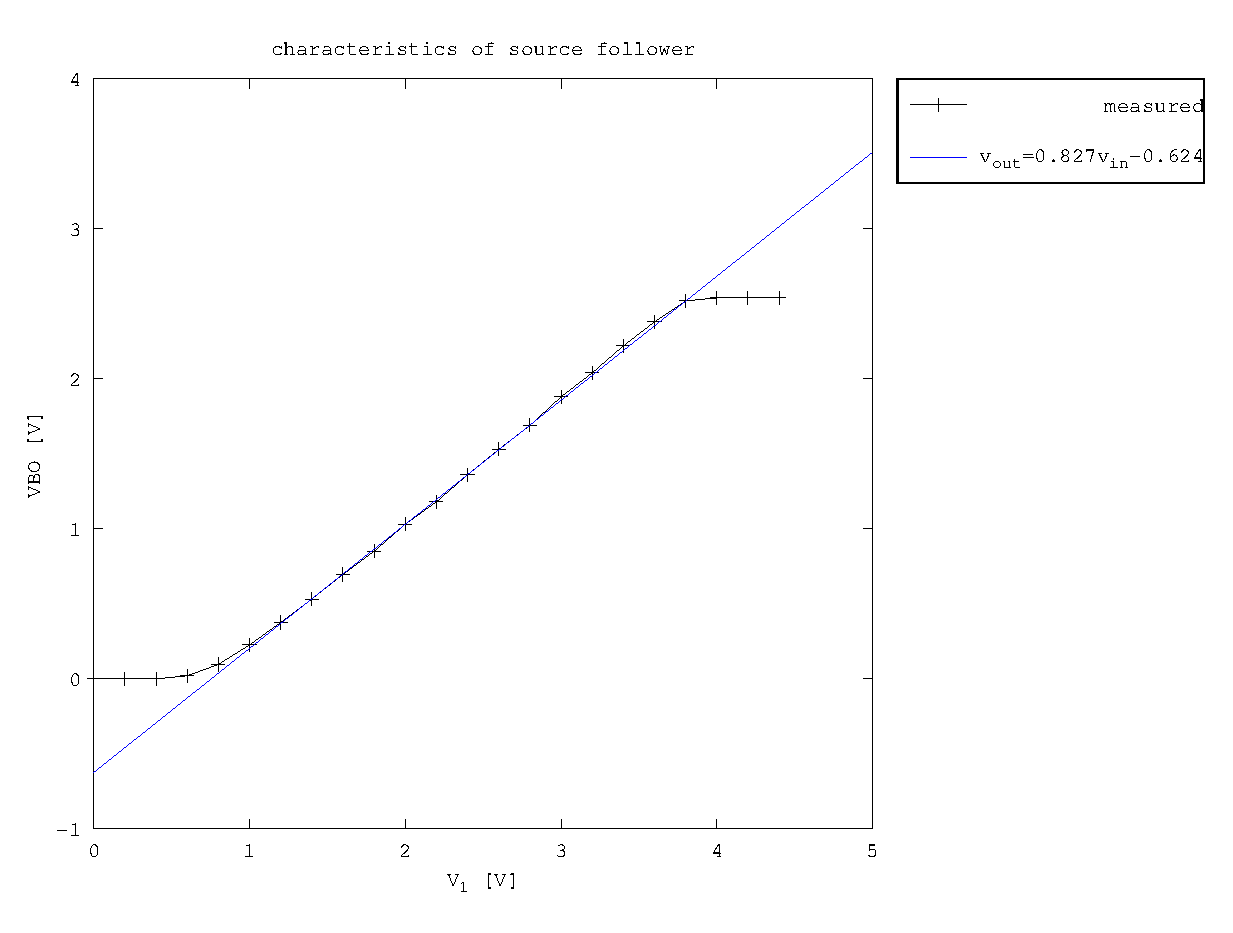
\includegraphics[width=\textwidth]{fig/source_follower.eps}
            \caption[]
                {plot of the input voltage against VBO. This plot shows the characteristics of the voltage follower}    
                \label{fig:source_follower}
        \end{figure}


\subsection{Integrator}\label{ssec:dynamic_integrator}
The measurements of the behavior of the integrator are devided into three sections. \Cref{sssec:standard_behavior} will focus on the output of the ROIC for low currents. \Cref{sssec:high_current_behavior} will do the same, but this time for currents that are a lot higher. Finally \cref{sssec:VBO_behavior} will look at the behavior of VBO, and investigate the viability of using the input follower as a secondary readout. Note that all plots are not what is directly observed at the output. All results have compensation for the behavior of the source followers.

\subsubsection{Standard behavior}\label{sssec:standard_behavior}
This test aims to address the basic relationship between input current and output voltage. \Cref{tkz:integrator_test} shows the setup used for this test. Channel 8 was used, so the end of the $20\,M\Omega$ resistor is connected to IN[8], and probes are connected to OUT[8] and VBO[8]. 

\begin{figure}[H]
\centering

\usetikzlibrary{shapes,snakes}

\newcommand*{\Vg}{Vg\\ $\color{red}4.5\,V$}
\newcommand*{\Rst}{\textbf{Rst[3]}\\ $\color{blue}reset$} 
\newcommand*{\Res}{Res\\ $\color{red}0.86\,V$}
\newcommand*{\VDD}{VDD3.3\\ $\color{red}3.3\,V$}
\newcommand*{\IN}{$\color{blue}V_{in}$}
\newcommand*{\OUT}{$\color{blue}V_{out}$}
\newcommand*{\VBO}{\color{blue}\textbf{VBO[8]} $\color{red}1.4\,V$}
\newcommand*{\gnd}{gnd\\ $\color{red}0\,V$}
\newcommand*{\C}{$\color{blue}C$}




\tikzstyle{dot} = [draw,shape=circle,fill=black, scale =.3]
\tikzstyle{l_arrow} = [draw,fill = black, regular polygon,regular polygon sides=3, rotate=-90, anchor=south, scale=.5] 
\tikzstyle{l_text} = [anchor=south west]
\tikzstyle{r_arrow} = [draw,fill = black, regular polygon,regular polygon sides=3, rotate=90, anchor=south, scale=.5] 
\tikzstyle{r_text} = [anchor=south east]
\begin{tikzpicture}[scale=1, every node/.style={scale=1}]




\draw[dashed]  (-0.5,5.5) rectangle (0.5,-2);
\node[align=center, anchor=south] at (0,5.5) {voltage\\limiter};

\draw[dashed]  (1.25,5.5) rectangle (5.25,-2);
\node[align=center, anchor=south] at (3.25,5.5) {integrator};

\draw[dashed]  (5.75,5.5) rectangle (9.25,-2);
\node[align=center, anchor=south] at (7.5,5.5) {current mirrors};

%\draw (0,0) to node[nfet]{};

%\draw (0,0) to (mos1.s);
\node(Vg)[nfet, rotate=-90] at (0,2.5) {};
\node[nfet, rotate=-90] (Reset) at (2.5,2) {};
\node[pfet] (CM_H1) at (5,3) {};
\node[nfet] (CM_L1) at (5,-1) {};
\node[nfet] (CM_H2) at (7,3) {};
\node[nfet] (CM_L2) at (7,-1) {};
\node[nfet] (CM_H3) at (9,3) {};
\node[nfet] (CM_L3) at (9,-1) {};



\draw (-1,2.5) node[anchor=east, align=center]{} to (Vg.S);
\draw (Vg.G) |- (0,4.5) node[anchor=south, align=center]{\Vg};
\draw (Vg.B) |- (1,2.5) node[dot]{} |- (CM_H1.G); %top
\draw (1,2.5) |- (1,0.5)  to [C=\C](4,0.5) -| (CM_H1.D);
\draw (1.5,0.5) node[dot]{} -| (1.5,2) |- (Reset.B);
\draw (Reset.G) to (2.5,4.5) node[anchor=south, align=center]{\Rst};
\draw (Reset.D) -| (3.5,0.5) node[dot]{};
\draw (5,0.5) node[dot]{} to (CM_L1.D);
\draw (CM_L1.G) to (4,4.5) node[anchor=south, align=center]{\Res}; 
\draw (CM_L1.S) to (CM_L2.S) to (7,-2.5) node[anchor=north, align=center]{\gnd};
\draw (CM_H1.B) |- (CM_H2.D) to (7,4.5) node[anchor=south, align=center]{\VDD};
\draw (CM_L2.G) |- (4,0) node[dot]{};
\draw (5,0.5) -| (CM_H2.G);
\draw (CM_L1.B) to (CM_L1.S);
\draw (CM_L2.B) to (CM_L2.S);
\draw (CM_H2.B) to (CM_L2.D);
\draw (CM_H3.B) to (CM_L3.D);
\draw (1,3)node[dot]{} |- (8,4) |- (CM_H3.G);
\draw (CM_H3.D) |- (CM_H2.D) node[dot]{};
\draw (CM_L3.S) |- (CM_L2.S) node[dot]{};
\draw (CM_L3.G) |- (6,0) node[dot]{};
\draw (7,1.5)node[dot]{} to (10,1.5) node[anchor=west, align=center]{\OUT};
%\draw (9,1)node[dot]{} to (10,1) node[anchor=west, align=center]{\VBO};

\draw (-2.5,2.5)node[anchor=east, align=center]{\IN} to [R=$20\,M\Omega$](-1,2.5);


\end{tikzpicture}

\caption{Schematic of ROIC channel template}
\label{tkz:integrator_test}
\end{figure}


\Cref{fig:slopes} shows the time versus voltage plot of both the VBO and OUT for a constant input voltage. The rising and falling slopes are the VBO and OUT respecively. The timescale of this plot does not allow for much inside in VBO, but it does show some interesting results for the behavior of OUT. When the reset switches, the input node immediately loses some charge. Note that the oscilloscope matches the rising edge of the reset signal to time is $0\,s$, so this drop is at $0\,s$. When the reset is switched, a capacitance is removed almost instantly. It is interesting to observe that the slope immediately after the rising edge of the reset signal is constant for all input voltages. This means that the observed slope is not limited by the reset transistor, but by the source follower that tries to keep up. This observed slope is therefore the maximum rate at which the output node can be pulled down in the current set-up. Also note that the slope gets steeper when the integrator capacitance decreases. This matches the expected behavior of $\Delta V = \frac{-q}{C}$.


\begin{figure}[h]
    \centering
    \begin{subfigure}[b]{0.475\textwidth}
            \centering
               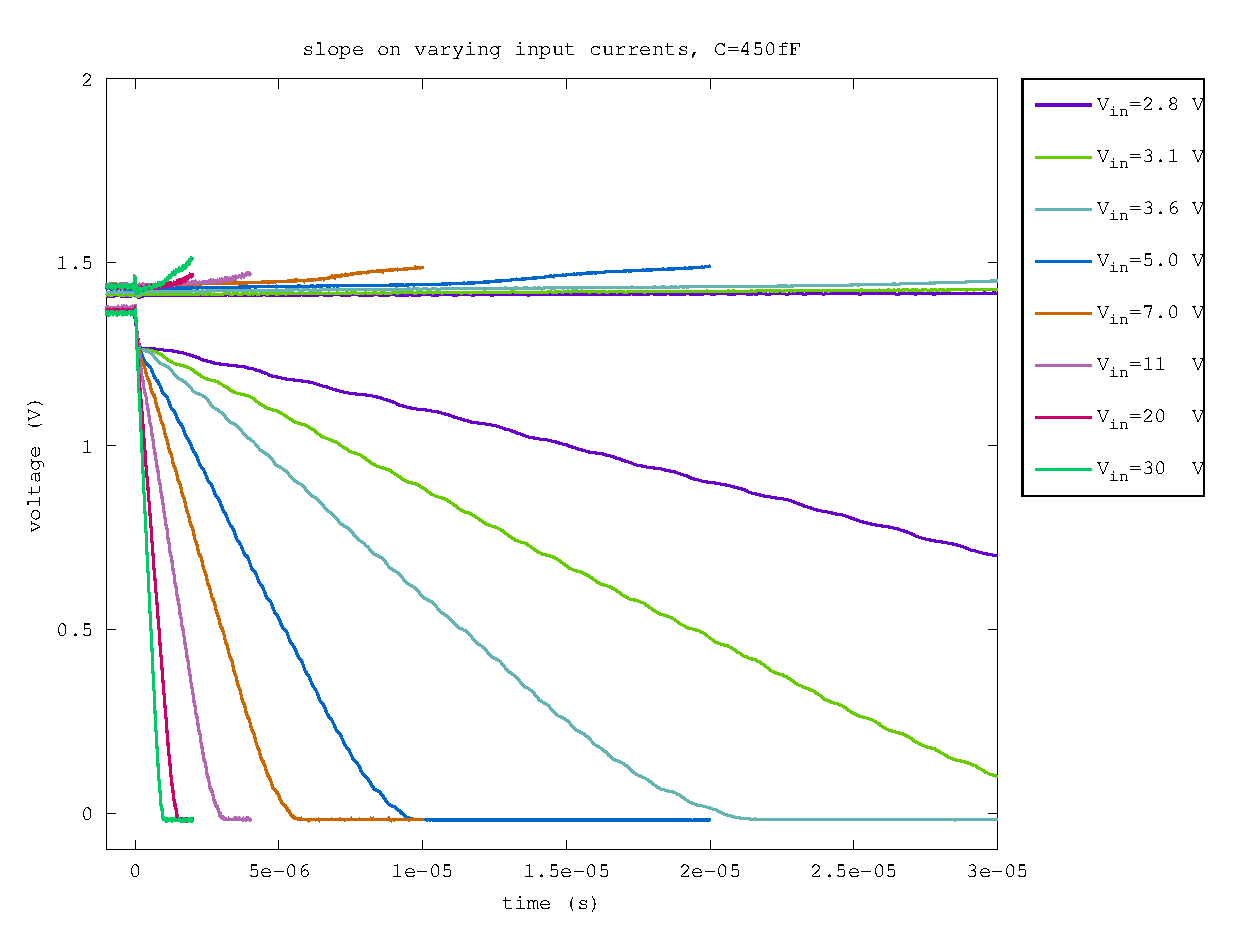
\includegraphics[width=\textwidth]{fig/slope_450fF.eps}
                    \caption[Network2]%
                        {$C=450\,fF$}    
                            \label{fig:slopes_450fF}
                        \end{subfigure}
                        \hfill
                        \begin{subfigure}[b]{0.475\textwidth}  
                                \centering 
                                    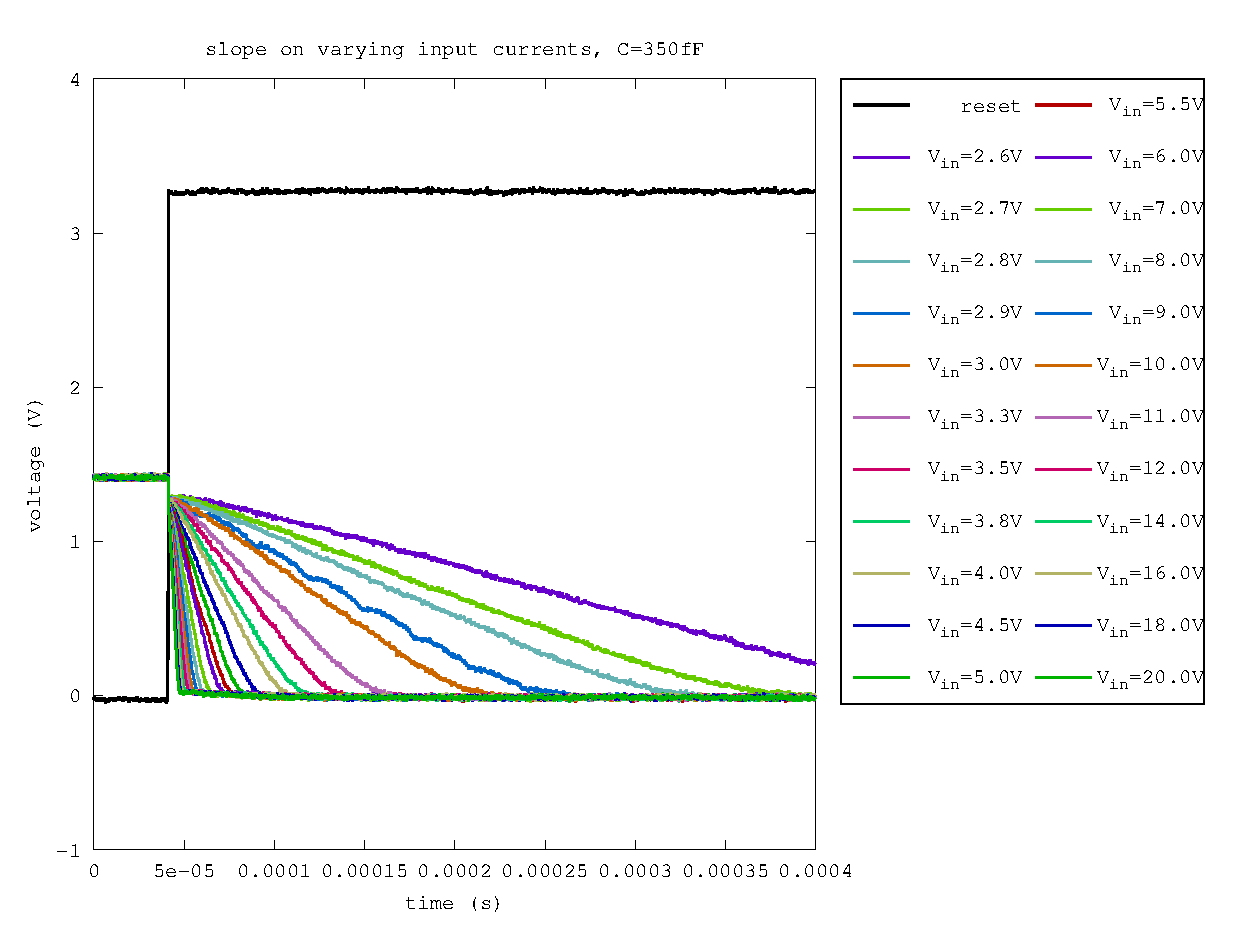
\includegraphics[width=\textwidth]{fig/slope_350fF.eps}
                                    \caption[]
                                        {$C=350\,fF$}    
                                        \label{fig:slopes_350fF}
                                \end{subfigure}
                            \vskip\baselineskip
                            \begin{subfigure}[b]{0.475\textwidth}   
                                \centering 
                                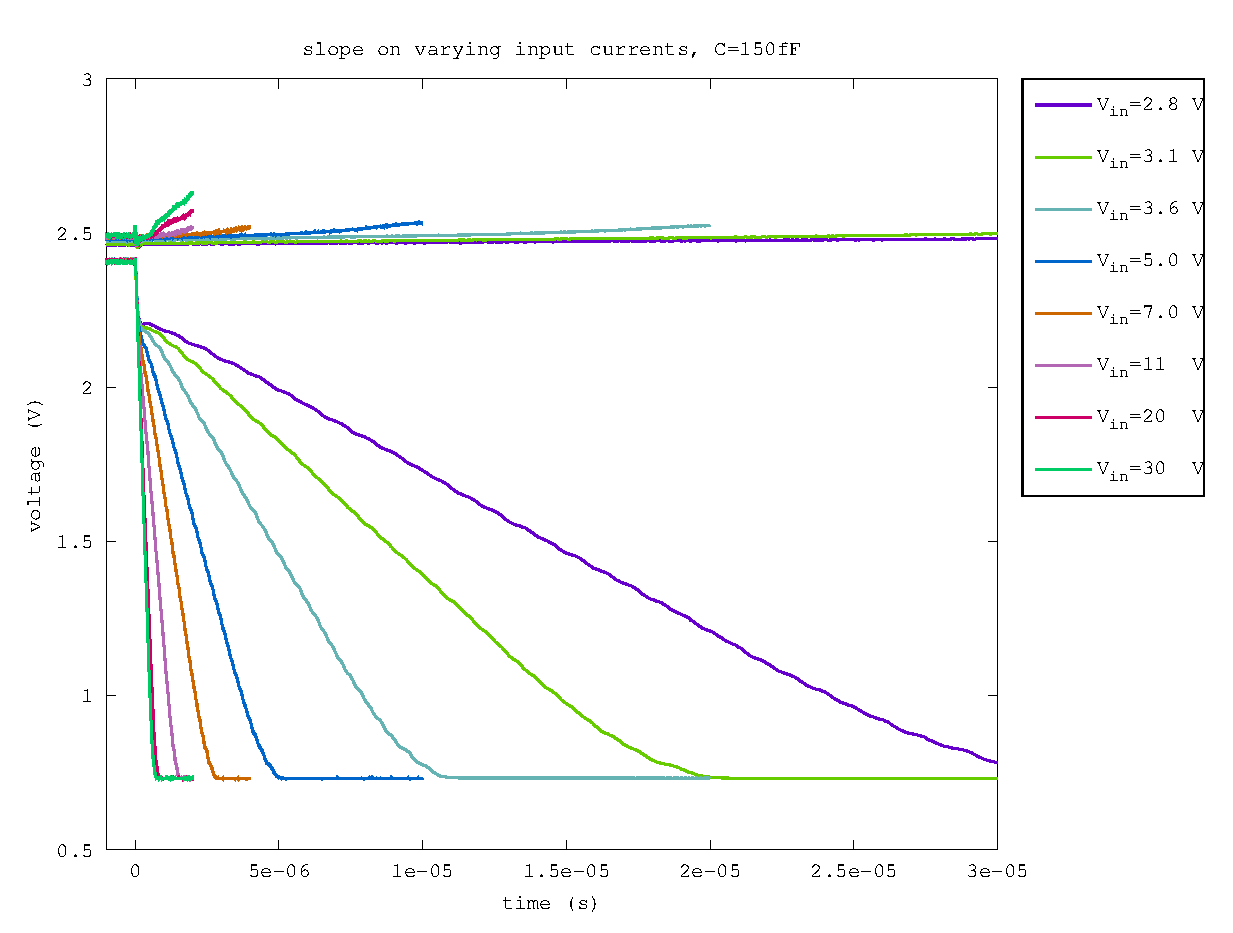
\includegraphics[width=\textwidth]{fig/slope_150fF.eps}
                                \caption[]
                                    {$C=150\,fF$}    
                                    \label{fig:slopes_150fF}
                            \end{subfigure}
                        \quad
                        \begin{subfigure}[b]{0.475\textwidth}   
                            \centering 
                            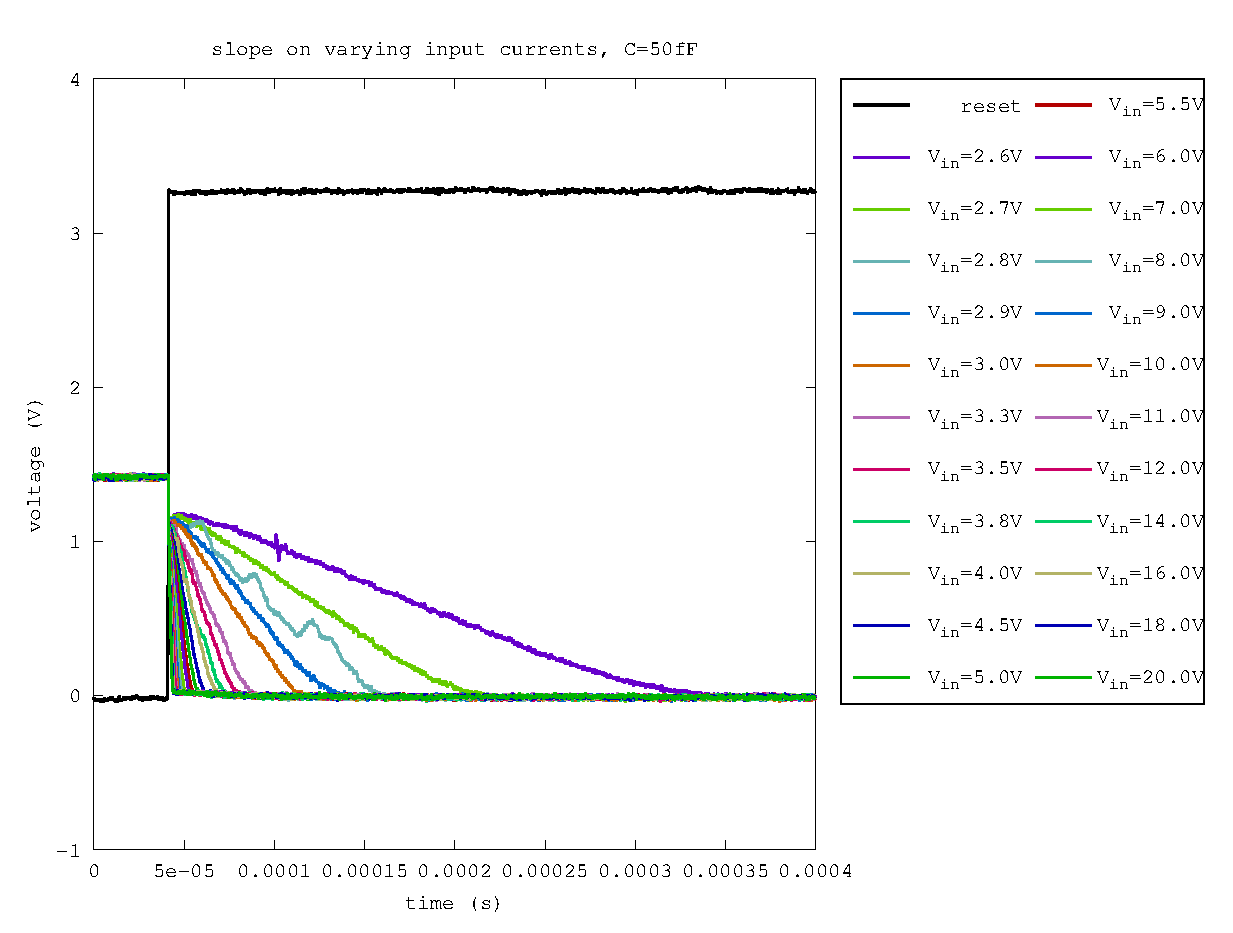
\includegraphics[width=\textwidth]{fig/slope_50fF.eps}
                            \caption[]
                                {$C=50\,fF$}    
                                \label{fig:slopes_50fF}
                        \end{subfigure}
                    \caption{Expected versus measured charge up times for different input voltages. The input voltage is connected to the input through a resistor of $20\,M\Omega$}
                \label{fig:slopes}
        \end{figure}
    
    \Cref{fig:charges} shows the same plot as \cref{fig:slopes}, but now the x axis is scaled with input current. This shows for \cref{fig:slopes_450fF} and \ref{fig:slopes_350fF} that the relationship between output voltage and charge is equal across different input voltages. For \cref{fig:slopes_150fF} and \ref{fig:slopes_50fF} however, one can see that the higher voltages lose this property. Another intersting observation is that when one looks closely at the plot, one can observe a small oscillation with a period that is constant with charge. Also the period is constant across different voltages. A hypothesis explaining this behavior has yet to be found.


    \begin{figure}[h]
    \centering
    \begin{subfigure}[b]{0.475\textwidth}
        \centering
        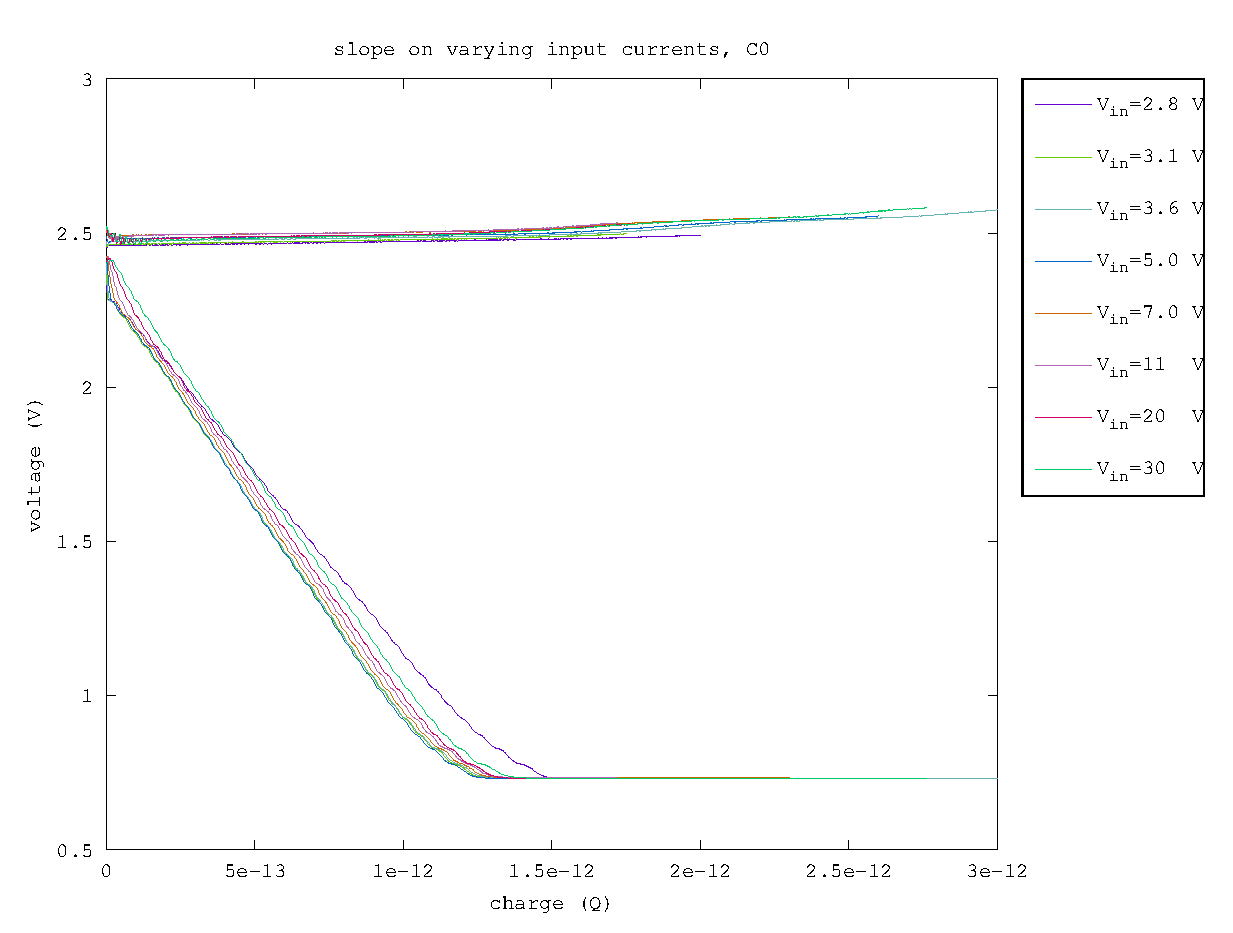
\includegraphics[width=\textwidth]{fig/charge_450fF.eps}
        \caption[Network2]%
        {$C=450\,fF$}    
        \label{fig:charges_450fF}
\end{subfigure}
\hfill
\begin{subfigure}[b]{0.475\textwidth}  
    \centering 
    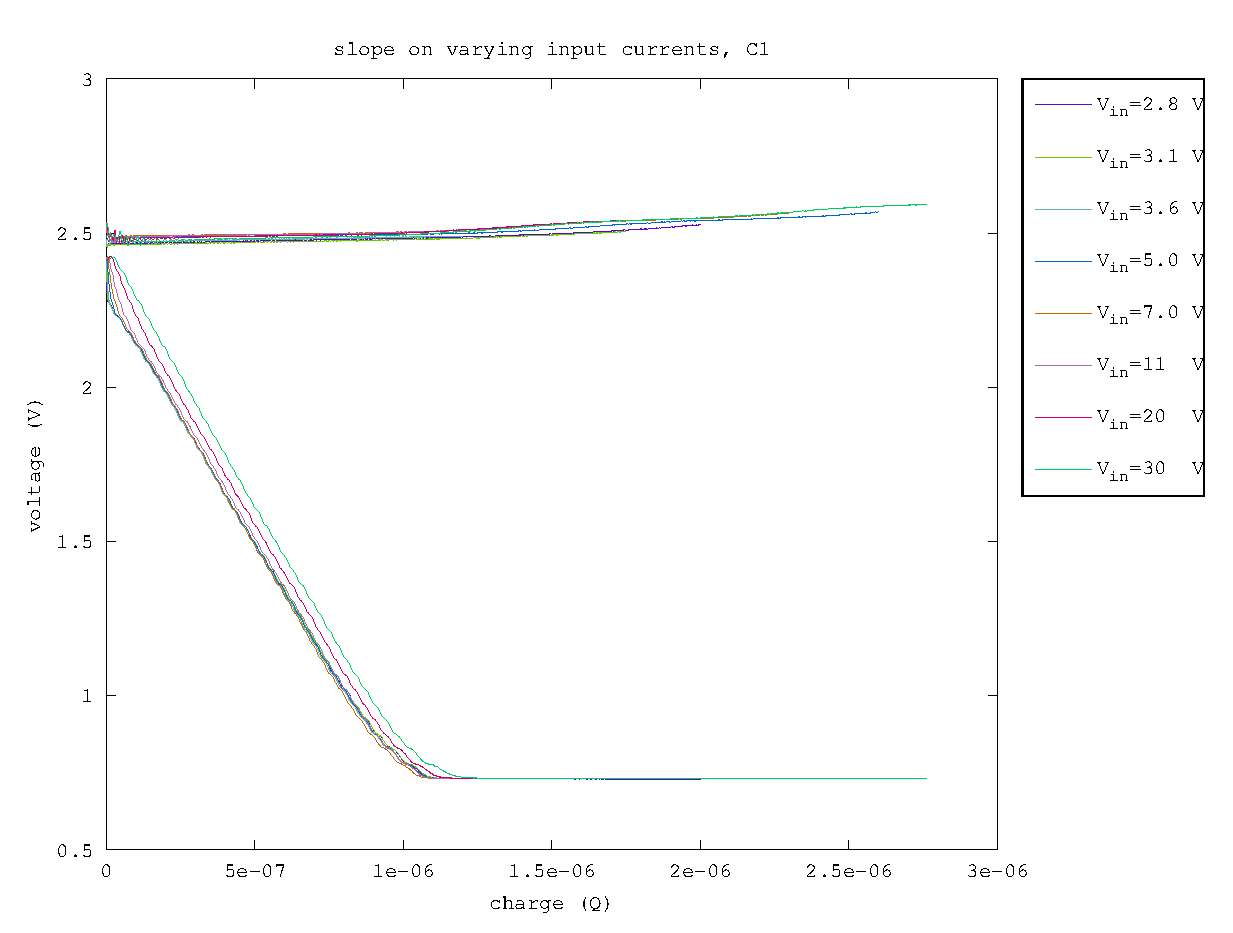
\includegraphics[width=\textwidth]{fig/charge_350fF.eps}
    \caption[]
        {$C=350\,fF$}    
        \label{fig:charges_350fF}
\end{subfigure}
\vskip\baselineskip
\begin{subfigure}[b]{0.475\textwidth}   
    \centering 
    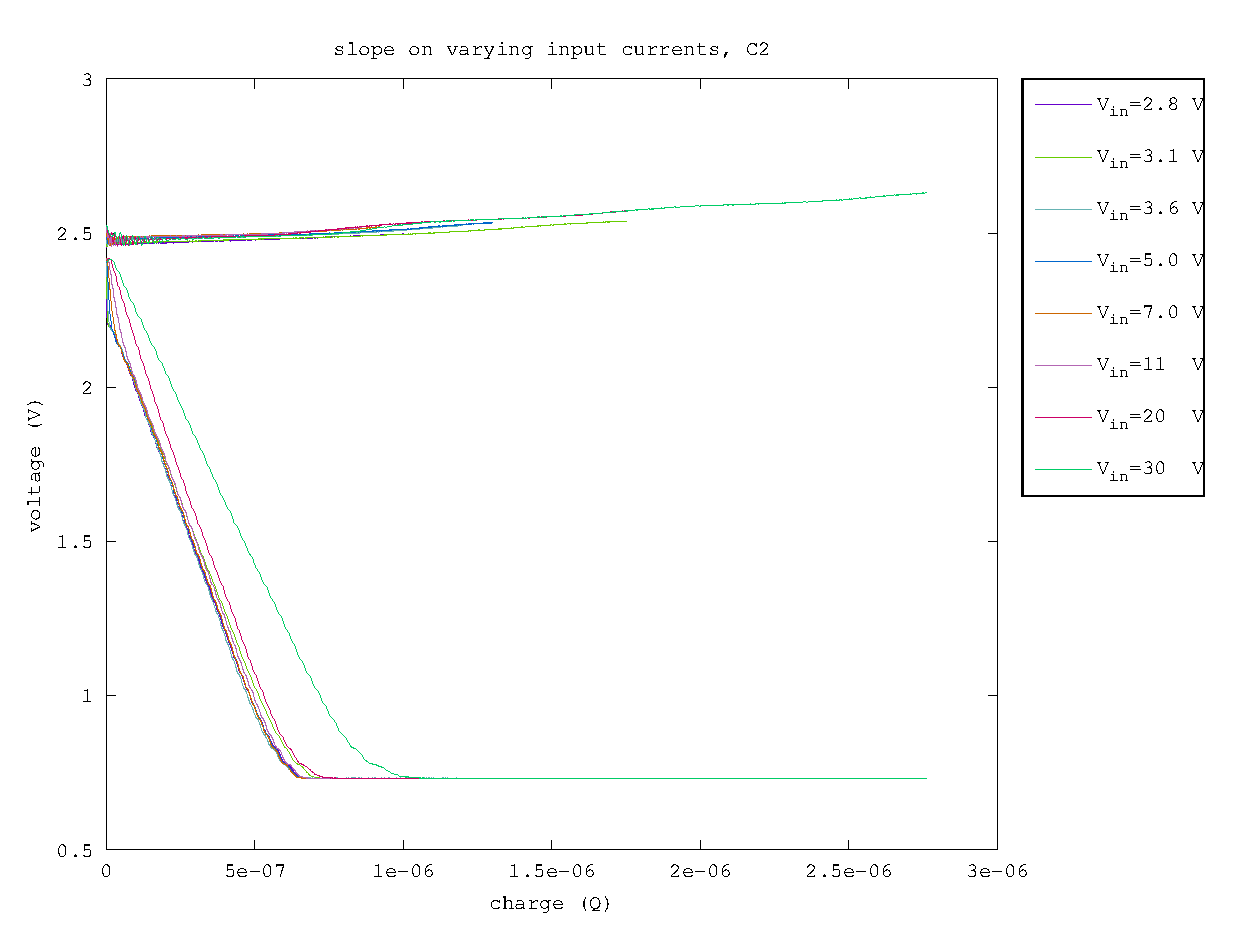
\includegraphics[width=\textwidth]{fig/charge_150fF.eps}
    \caption[]
        {$C=150\,fF$}    
        \label{fig:charges_150fF}
\end{subfigure}
\quad
\begin{subfigure}[b]{0.475\textwidth}   
    \centering 
    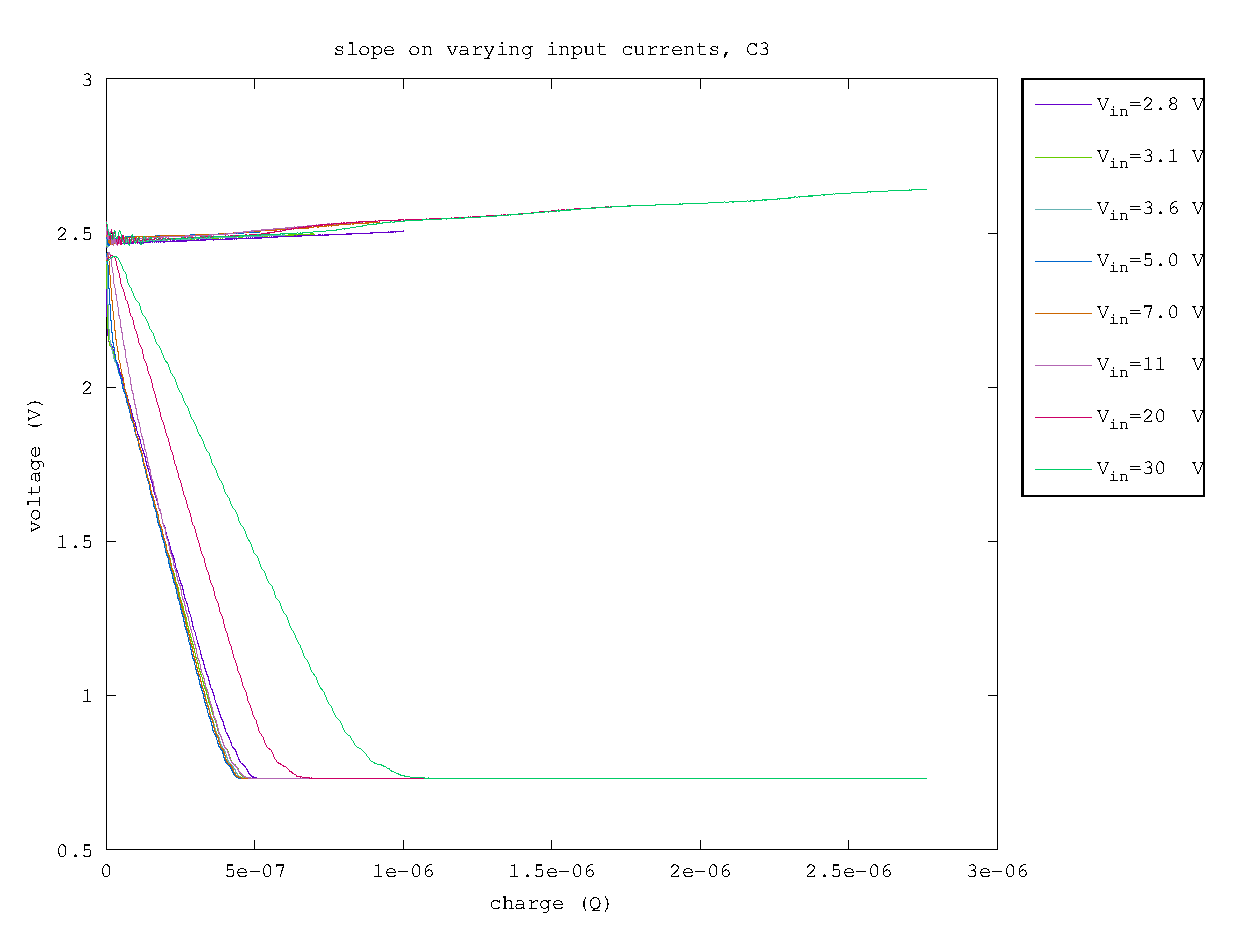
\includegraphics[width=\textwidth]{fig/charge_50fF.eps}
    \caption[]
        {$C=50\,fF$}    
        \label{fig:charges_50fF}
\end{subfigure}
\caption{This plot is showing charge versus voltage}
\label{fig:charges}
\end{figure}

\Cref{fig:d_slopes} shows the $\delta Q/\delta V$ against charge plots. Note that $\delta Q/\delta V$ is the capacitance. One can observe that while the capacitance is charging, the full value of the capacitancec can be observed, and when the capacitance is comopletely decharged, it behaves as if it is not there. One can use these plots to estimate the integration capacitance. The capitance for \cref{fig:charges_450fF}, \ref{fig:charges_350fF}, \ref{fig:charges_150fF} and \ref{fig:charges_50fF} are approxiately $450\,fF$, $350\,fF$, $220\,fF$ and $180\,fF$ respectively.


\begin{figure}[h]
\centering
\begin{subfigure}[b]{0.475\textwidth}
    \centering
    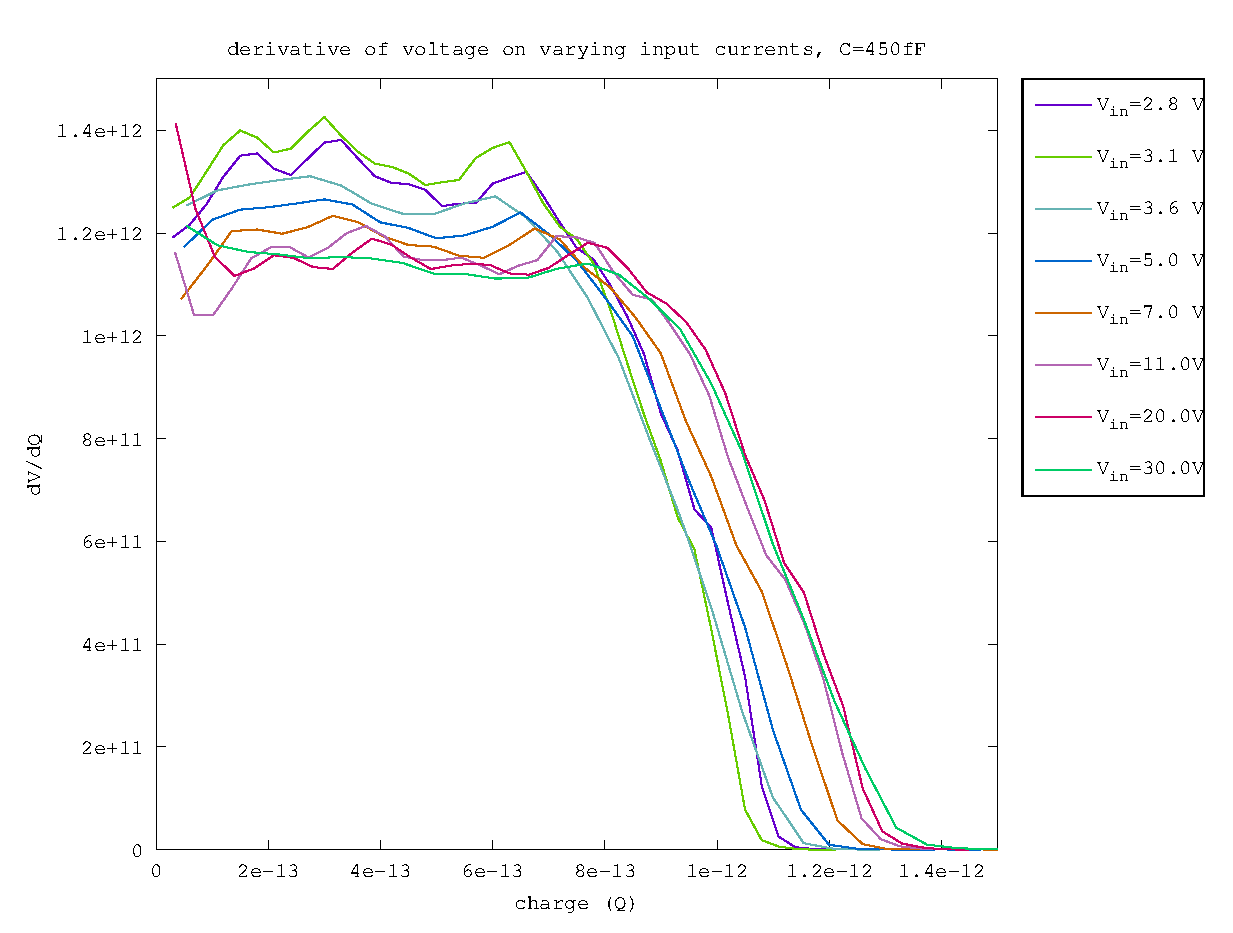
\includegraphics[width=\textwidth]{fig/d_slope_450fF.eps}
    \caption[Network2]%
    {$C=450\,fF$}    
    \label{fig:d_slopes_450fF}
\end{subfigure}
\hfill
\begin{subfigure}[b]{0.475\textwidth}  
    \centering 
    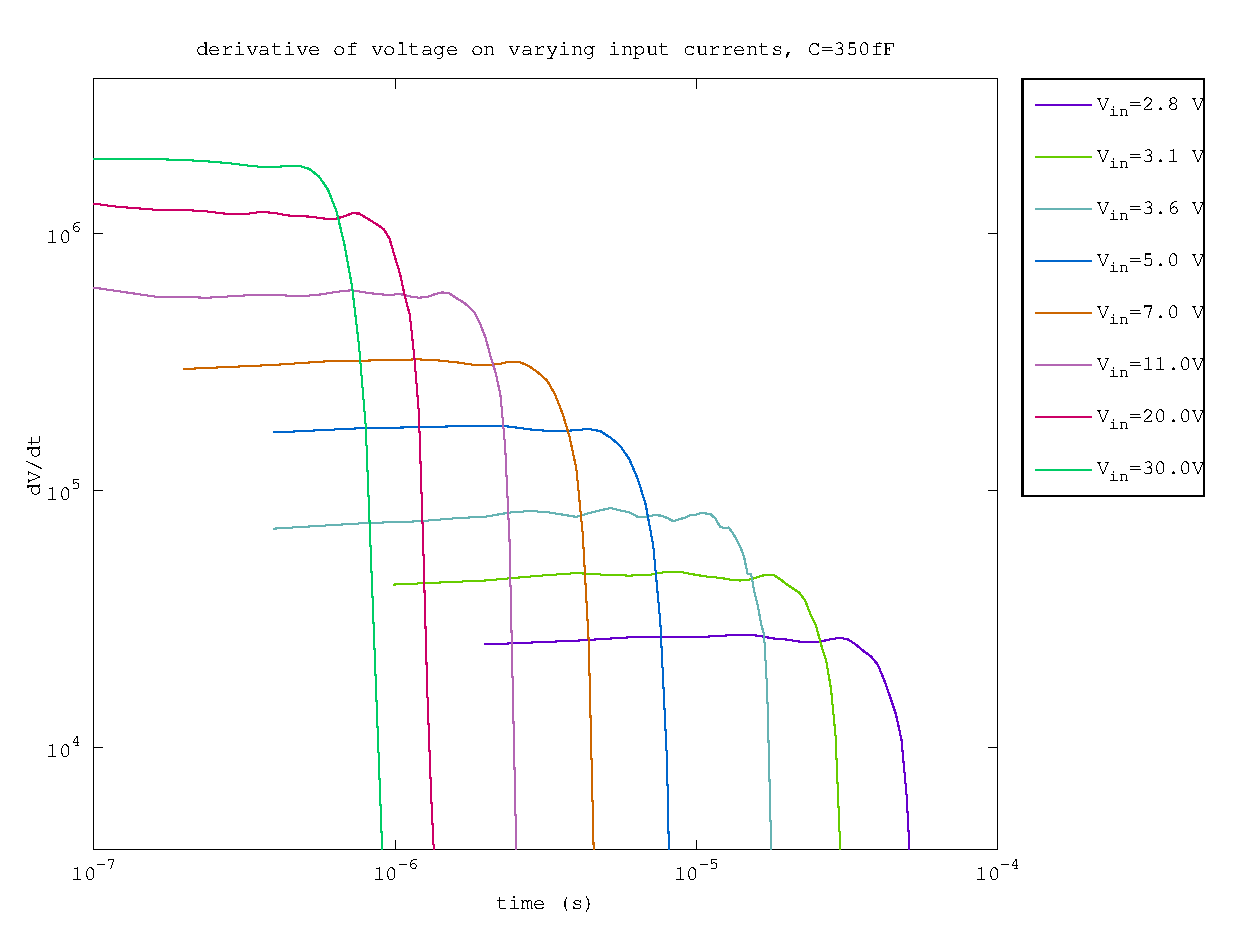
\includegraphics[width=\textwidth]{fig/d_slope_350fF.eps}
    \caption[]
        {$C=350\,fF$}    
        \label{fig:d_slopes_350fF}
\end{subfigure}
\vskip\baselineskip
\begin{subfigure}[b]{0.475\textwidth}   
    \centering 
    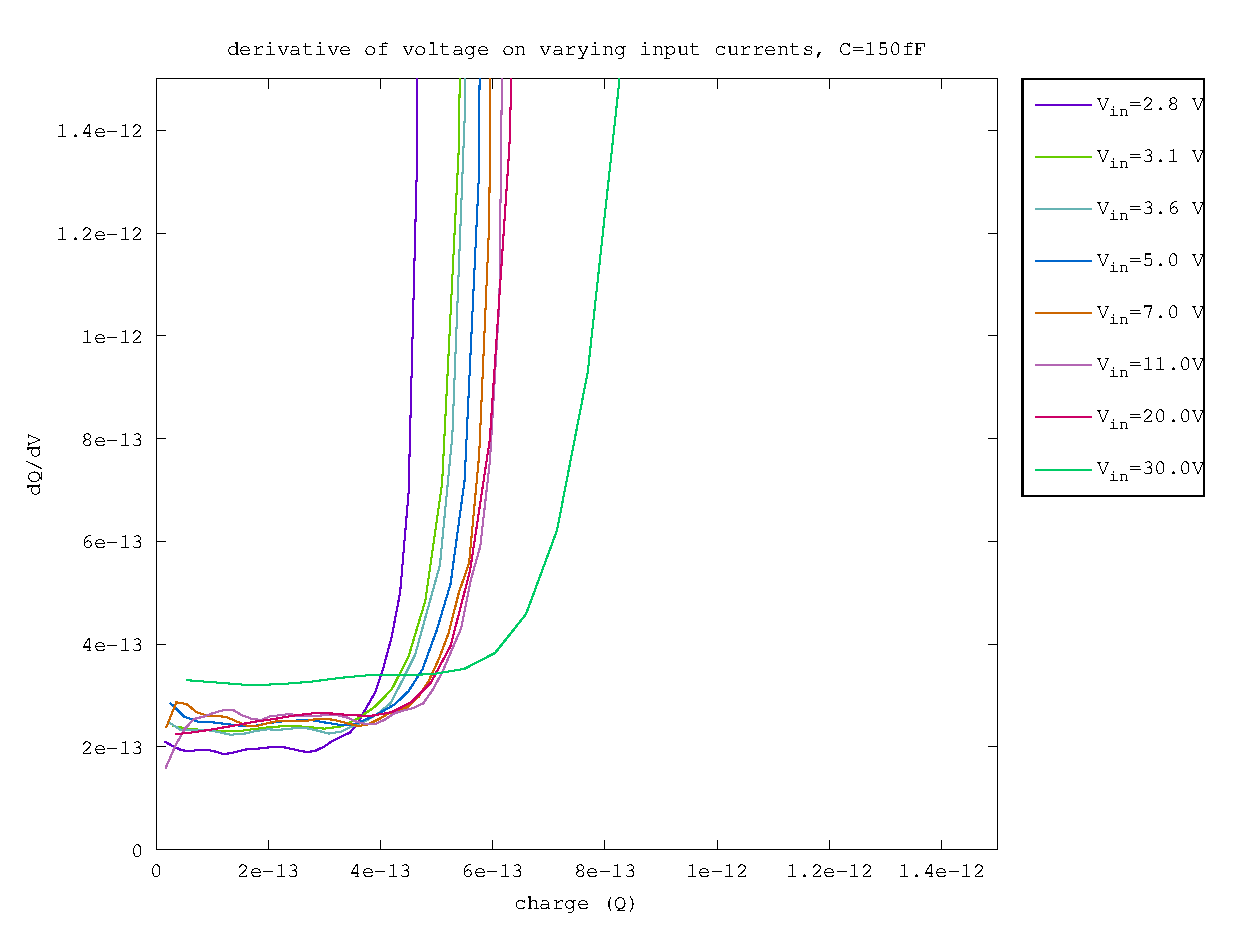
\includegraphics[width=\textwidth]{fig/d_slope_150fF.eps}
    \caption[]
        {$C=150\,fF$}    
        \label{fig:d_slopes_150fF}
\end{subfigure}
\quad
\begin{subfigure}[b]{0.475\textwidth}   
    \centering 
    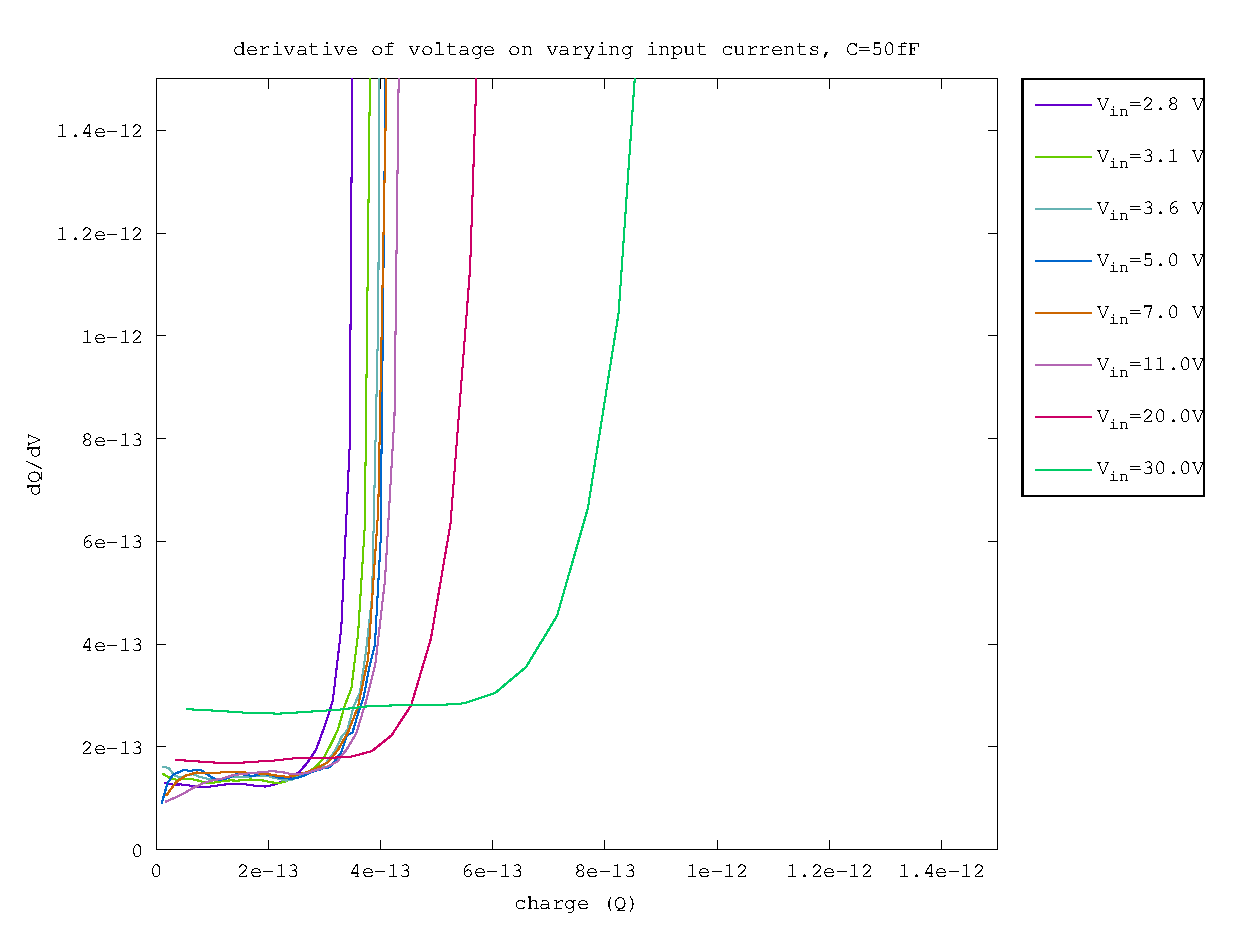
\includegraphics[width=\textwidth]{fig/d_slope_50fF.eps}
    \caption[]
        {$C=50\,fF$}    
        \label{fig:d_slopes_50fF}
\end{subfigure}
\caption{The plot shows dv/dt against time. The plot is in log scale, which allows for an easy read on the maximum slope and the time needed to discharge the integrator capacitance. }
\label{fig:d_slopes}
\end{figure}



\Cref{fig:e_vs_m} shows $\delta V / \delta t$ against input voltage for all capacitances. One can observe that all four have different slopes at first, but there appears to be a trend that they all converge to a value of $\delta V/\delta t \approx 3.2\cdot10^6$.


\begin{figure}[h]
    \centering
    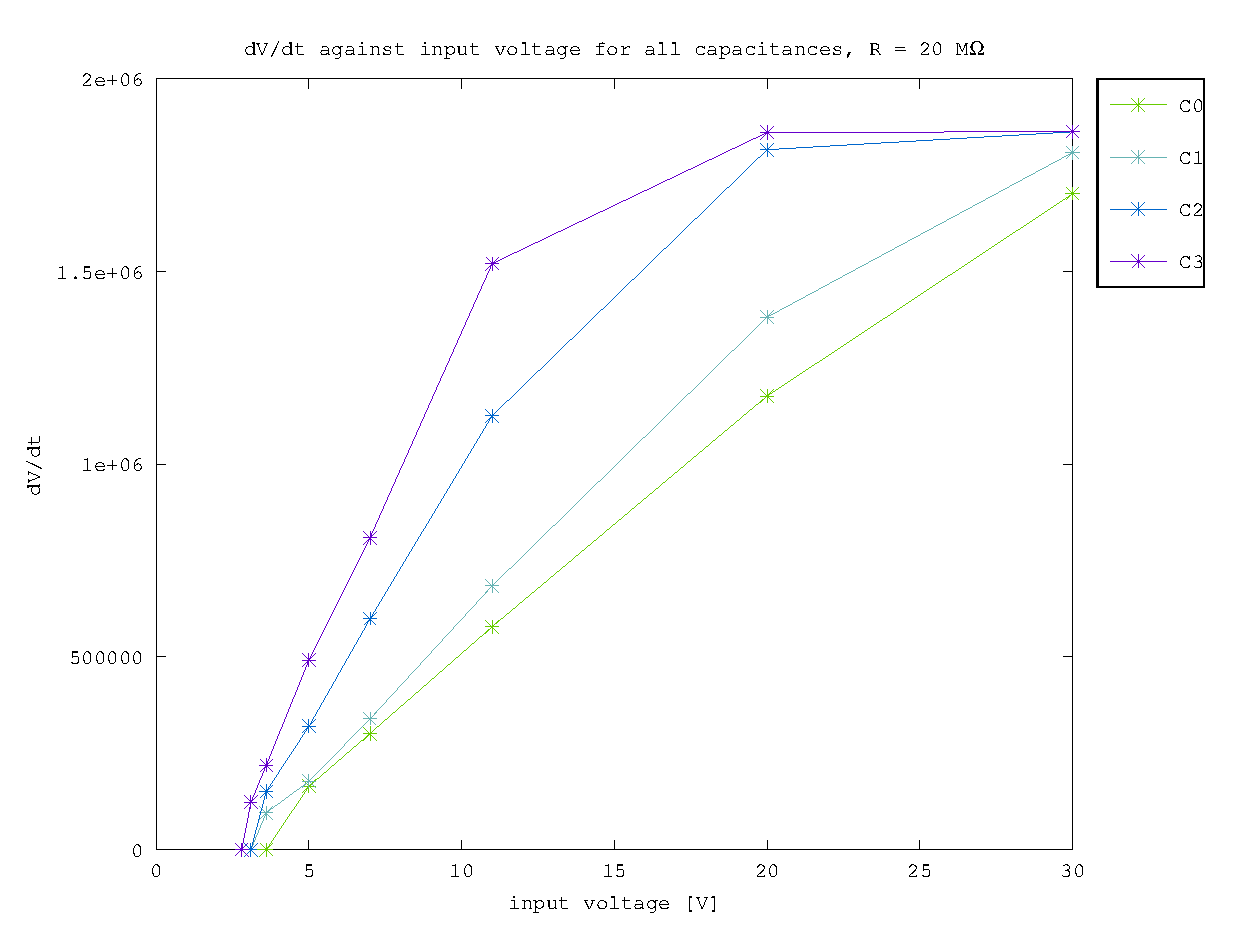
\includegraphics[width=\textwidth]{fig/vin_vs_time_sat.eps}
    \caption[]
        {dV/dt against input voltage for all four capacitances. The x indicate the measurements.}    
        \label{fig:e_vs_m}
\end{figure}

\clearpage
\subsubsection{High current behavior}\label{sssec:high_current_behavior}
In this section the $20\,M\Omega$ input resistor is replaecd with a $4\,M\Omega$ resistor. The main goal is to observe the ROIC for very large currents.


\Cref{fig:bre_slopes} shows the same plot as \cref{fig:slopes}, but this time with larger currents. Where a minimum slope could be observed at \cref{fig:slopes}, it is more prevalent here. This also shows more information about the behavior of VBO. For small voltages the VBO does not increase, but as the voltages get larger, one can observe that the voltages of VBO start rising when the OUT is done with decharging. It is also interesting to note that VBO seems to be not affected by the minimum slope at OUT. This gives rise to the hypothesis that the OUT is limited by the source follower. 

\begin{figure}[h]
    \centering
    \begin{subfigure}[b]{0.475\textwidth}
        \centering
        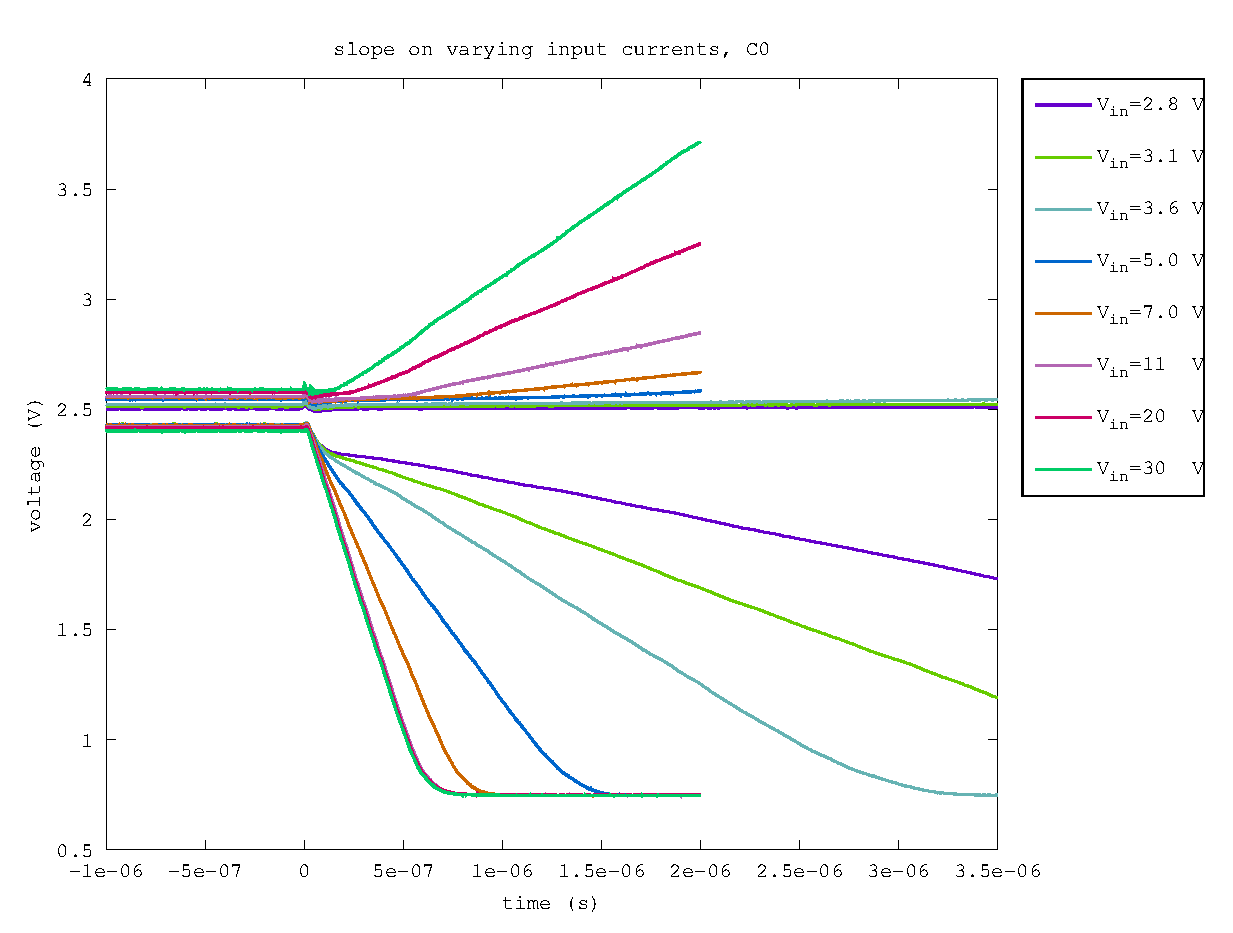
\includegraphics[width=\textwidth]{fig/bre_slope_450fF.eps}
        \caption[Network2]%
        {$C=450\,fF$}    
        \label{fig:bre_slopes_450fF}
    \end{subfigure}
    \hfill
    \begin{subfigure}[b]{0.475\textwidth}  
        \centering 
        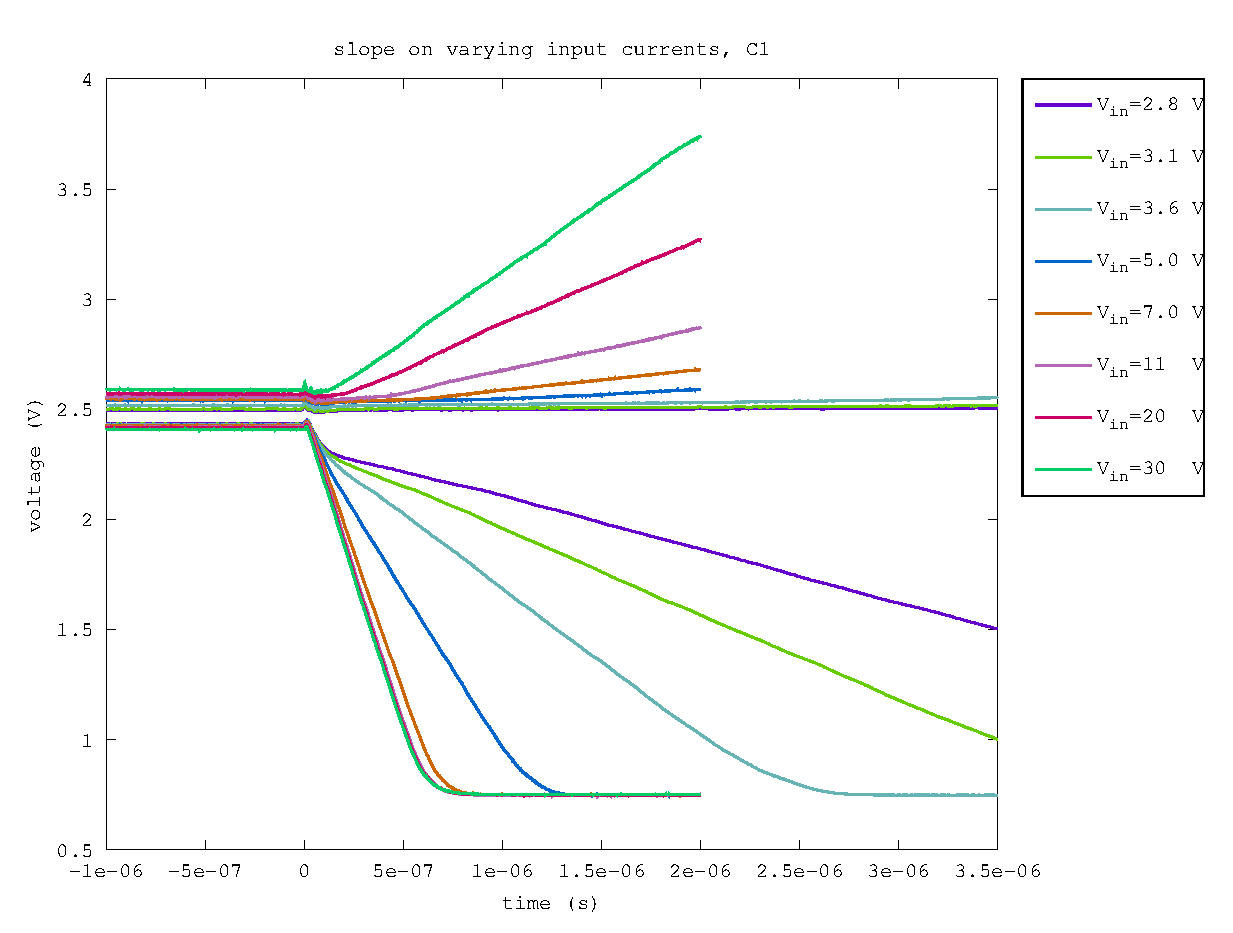
\includegraphics[width=\textwidth]{fig/bre_slope_350fF.eps}
        \caption{$C=350\,fF$}    
        \label{fig:bre_slopes_350fF}
    \end{subfigure}
    \vskip\baselineskip
    \begin{subfigure}[b]{0.475\textwidth}   
        \centering 
        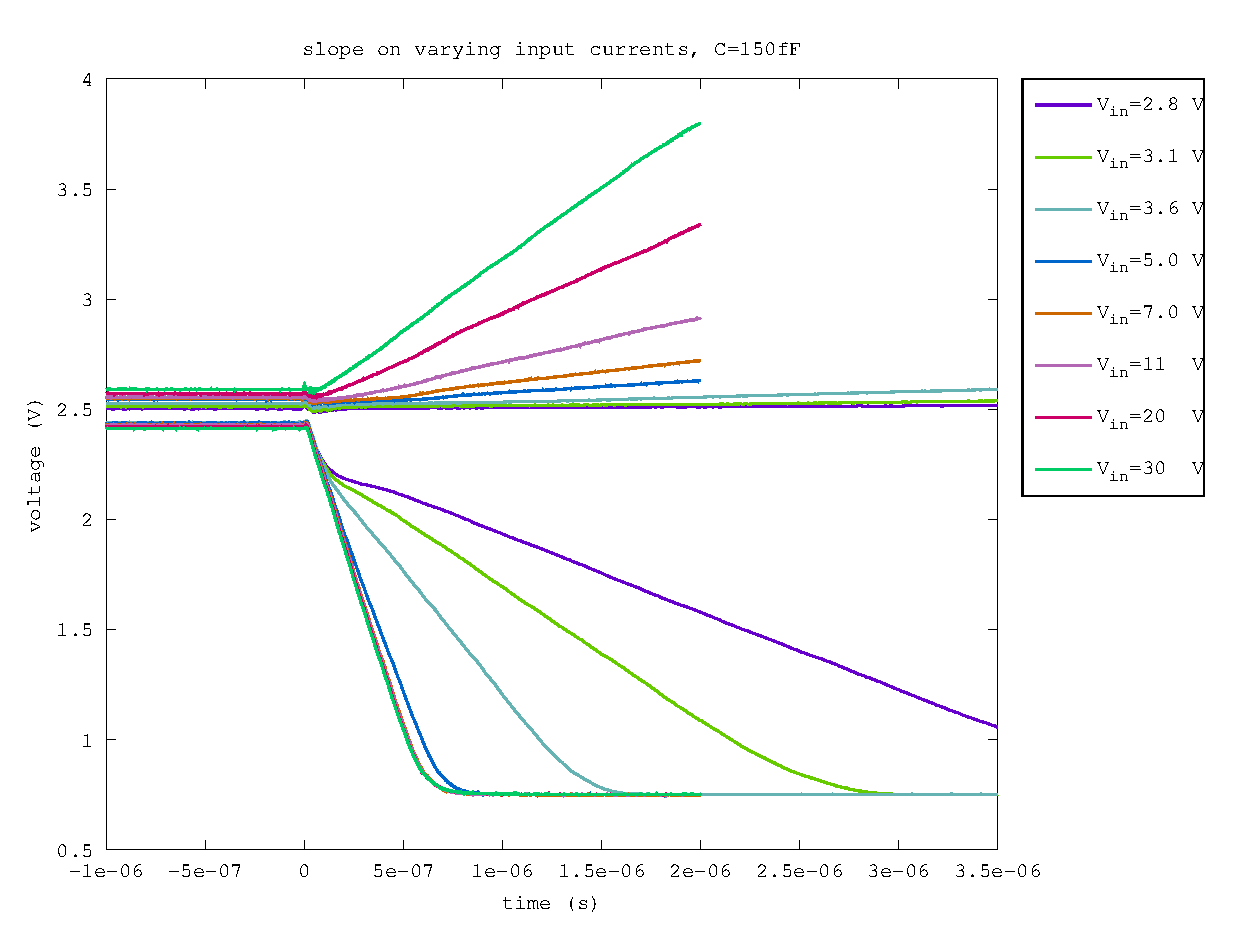
\includegraphics[width=\textwidth]{fig/bre_slope_150fF.eps}
        \caption{$C=150\,fF$}    
        \label{fig:bre_slopes_150fF}
    \end{subfigure}
    \quad
    \begin{subfigure}[b]{0.475\textwidth}   
        \centering 
        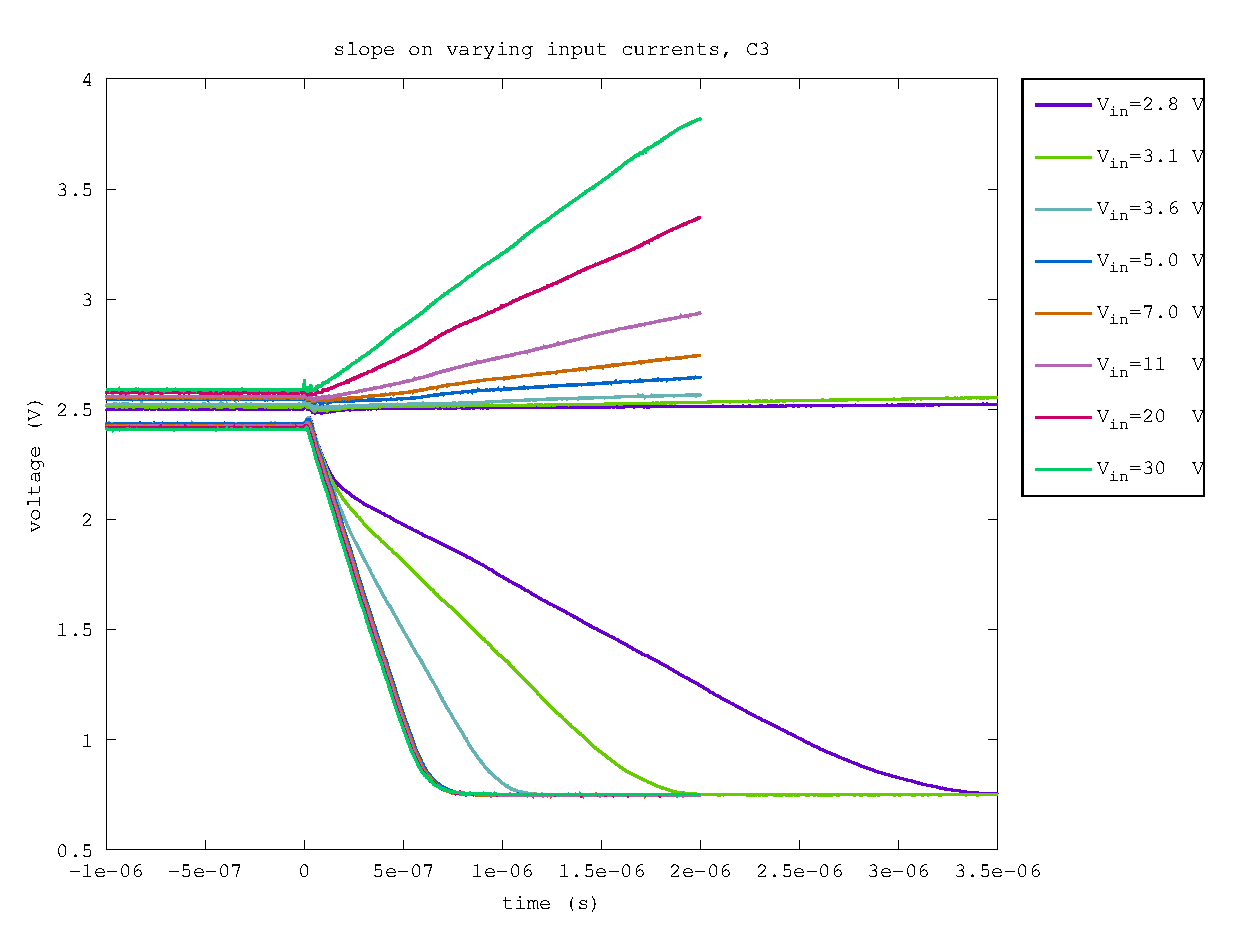
\includegraphics[width=\textwidth]{fig/bre_slope_50fF.eps}
        \caption{$C=50\,fF$}    
        \label{fig:bre_slopes_50fF}
    \end{subfigure}
    \caption{Expected versus measured charge up times for different input voltages. The input voltage is connected to the input through a resistor of $4\,M\Omega$}
    \label{fig:bre_slopes}
\end{figure}

\Cref{fig:bre_charges} shows a similar plot as in \cref{fig:charges} but with higher currents. In \cref{fig:charges} one could observe that all currents fitted to the same line, but deviated at higher currents. This effect is also observed here, but in a stronger form. Which is to be expected.

\begin{figure}[h]
    \centering
    \begin{subfigure}[b]{0.475\textwidth}
        \centering
        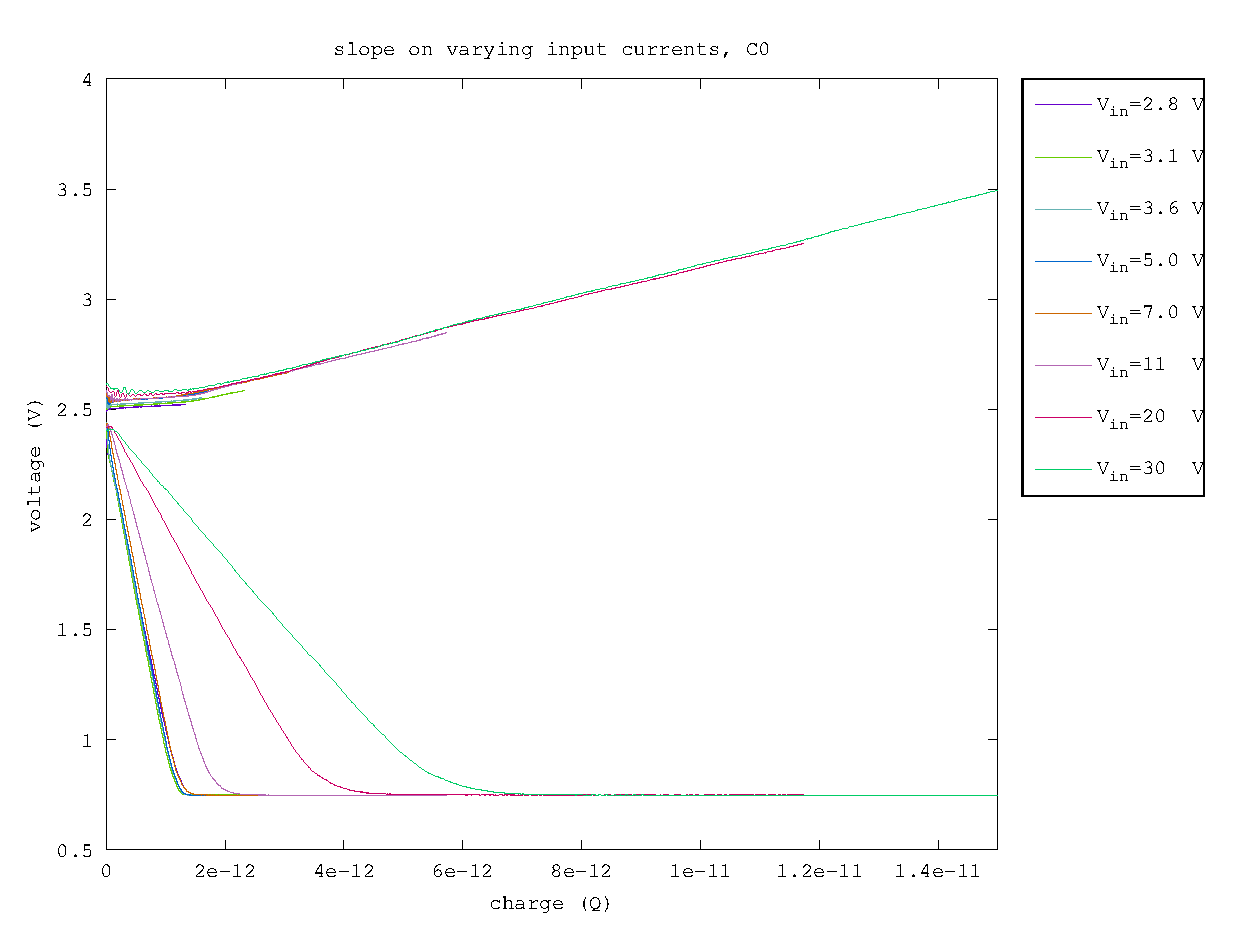
\includegraphics[width=\textwidth]{fig/bre_charge_450fF.eps}
        \caption[Network2]%
        {$C=450\,fF$}    
        \label{fig:bre_charges_450fF}
    \end{subfigure}
    \hfill
    \begin{subfigure}[b]{0.475\textwidth}  
        \centering 
        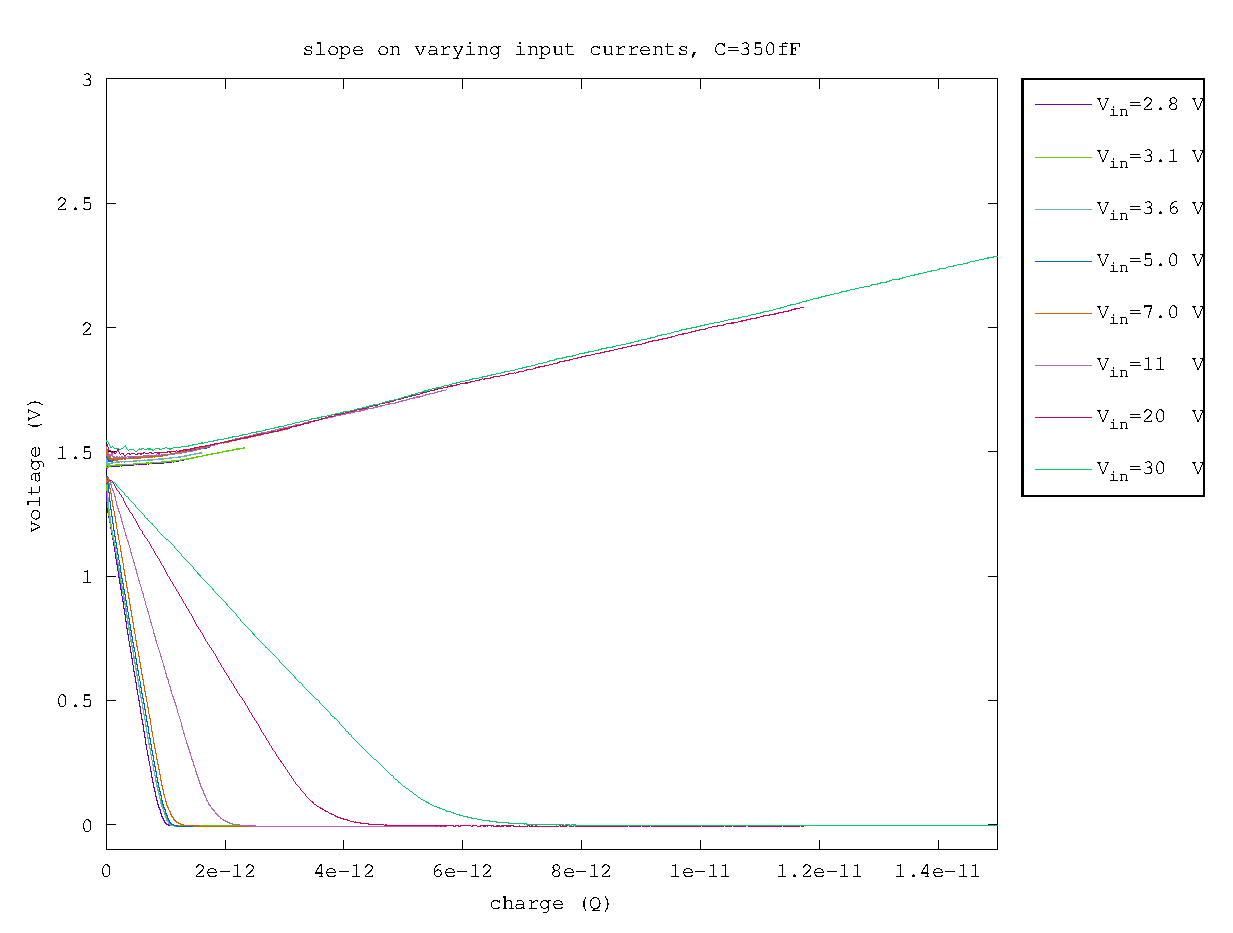
\includegraphics[width=\textwidth]{fig/bre_charge_350fF.eps}
        \caption{$C=350\,fF$}    
        \label{fig:bre_charges_350fF}
    \end{subfigure}
    \vskip\baselineskip
    \begin{subfigure}[b]{0.475\textwidth}   
        \centering 
        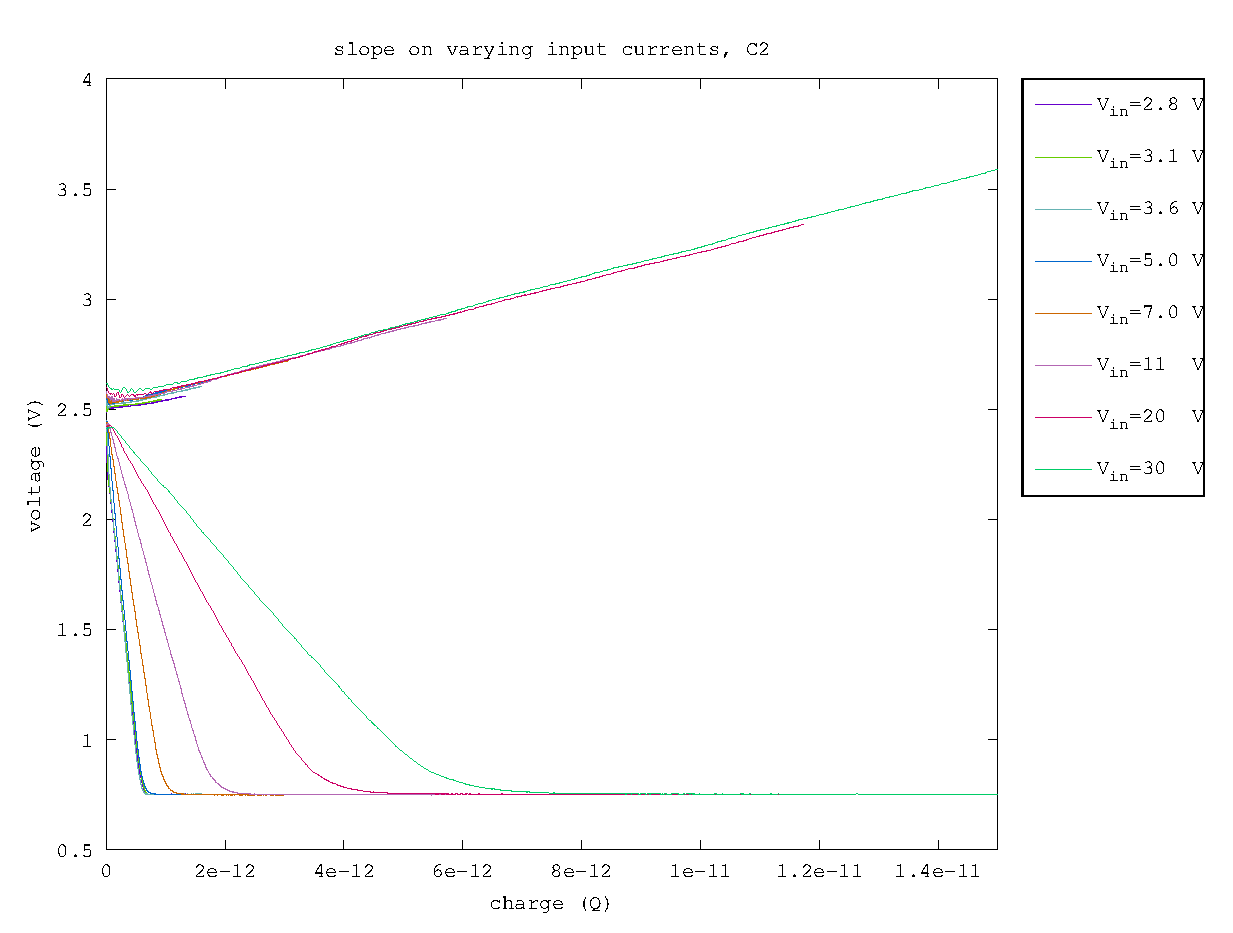
\includegraphics[width=\textwidth]{fig/bre_charge_150fF.eps}
        \caption{$C=150\,fF$}    
        \label{fig:bre_charges_150fF}
    \end{subfigure}
    \quad
    \begin{subfigure}[b]{0.475\textwidth}   
        \centering 
        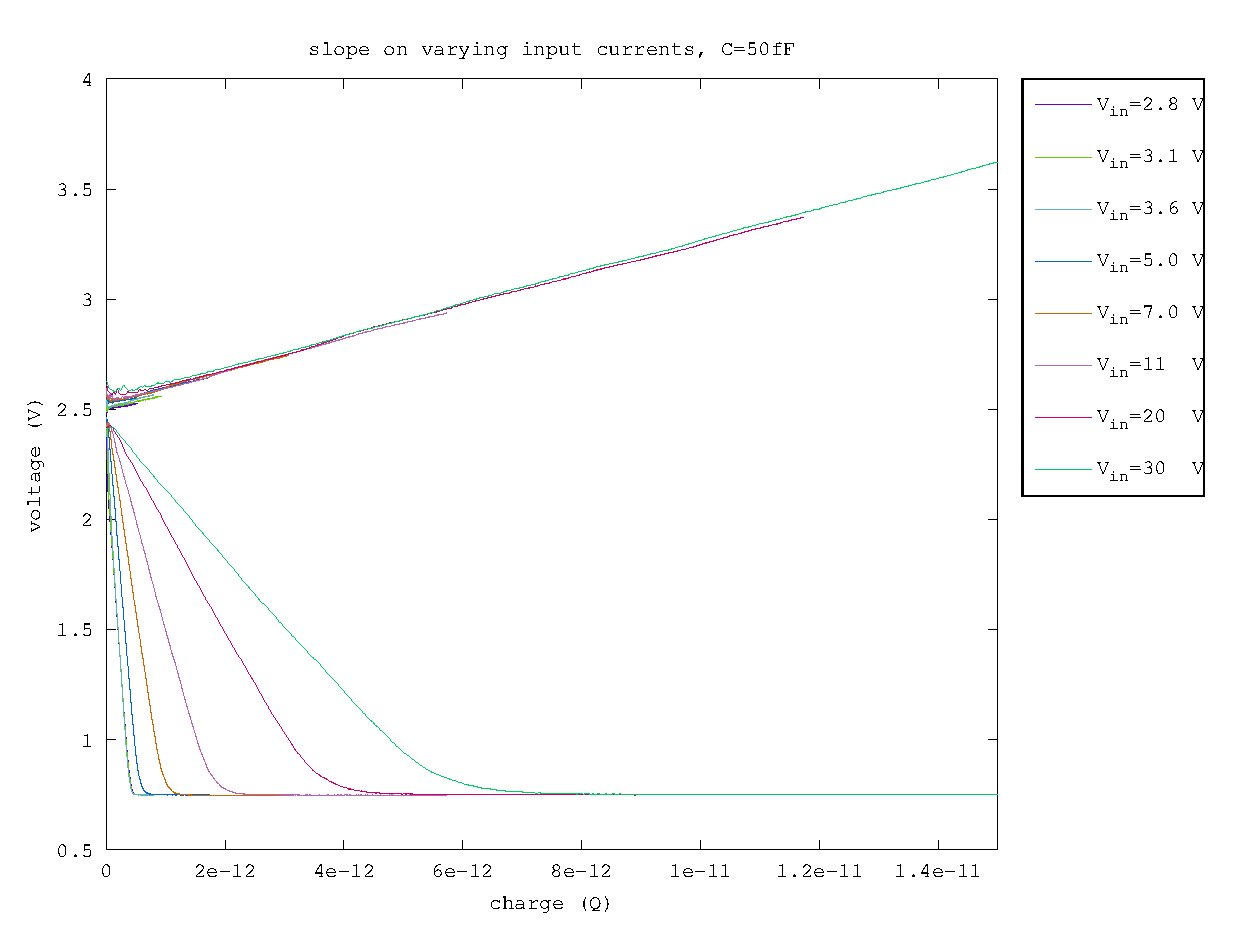
\includegraphics[width=\textwidth]{fig/bre_charge_50fF.eps}
        \caption {$C=50\,fF$}    
        \label{fig:bre_charges_50fF}
    \end{subfigure}
    \caption{This plot is showing charge versus voltage}
    \label{fig:bre_charges}
\end{figure}

\Cref{fig:bre_d_slopes} shows a plot of $\delta V/\delta Q$ against charge. Note that the behavior for the low voltages differ across the different capacitances, but that the high voltages are not affected by a change in capacitance. This observation agrees with the hypothesis that the output is not limited by the input current, but by the speed of the source follower at the output.

\begin{figure}[h]
    \centering
    \begin{subfigure}[b]{0.475\textwidth}
        \centering
        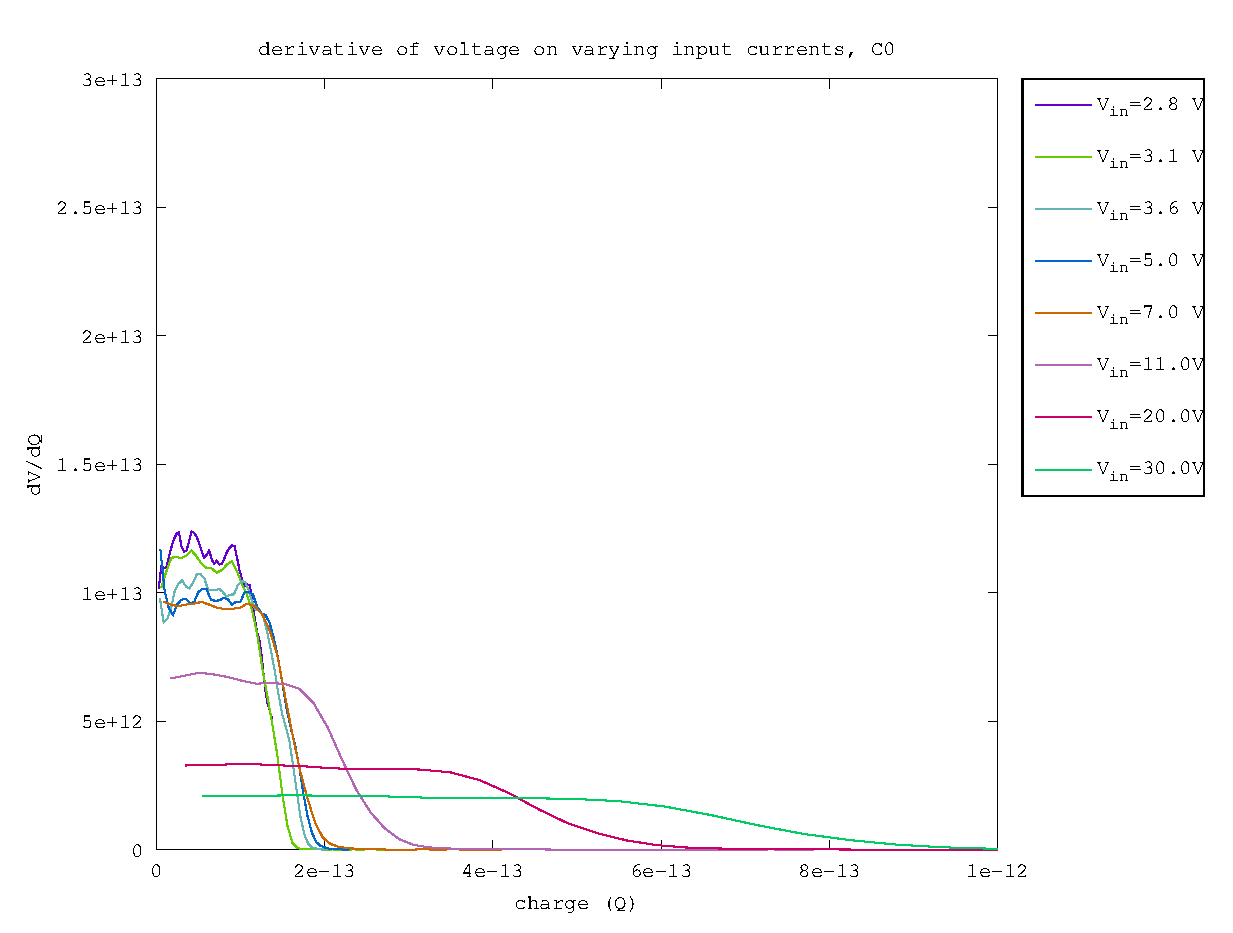
\includegraphics[width=\textwidth]{fig/bre_d_slope_450fF.eps}
        \caption[Network2]%
        {$C=450\,fF$}    
        \label{fig:bre_d_slopes_450fF}
    \end{subfigure}
    \hfill
    \begin{subfigure}[b]{0.475\textwidth}  
        \centering 
        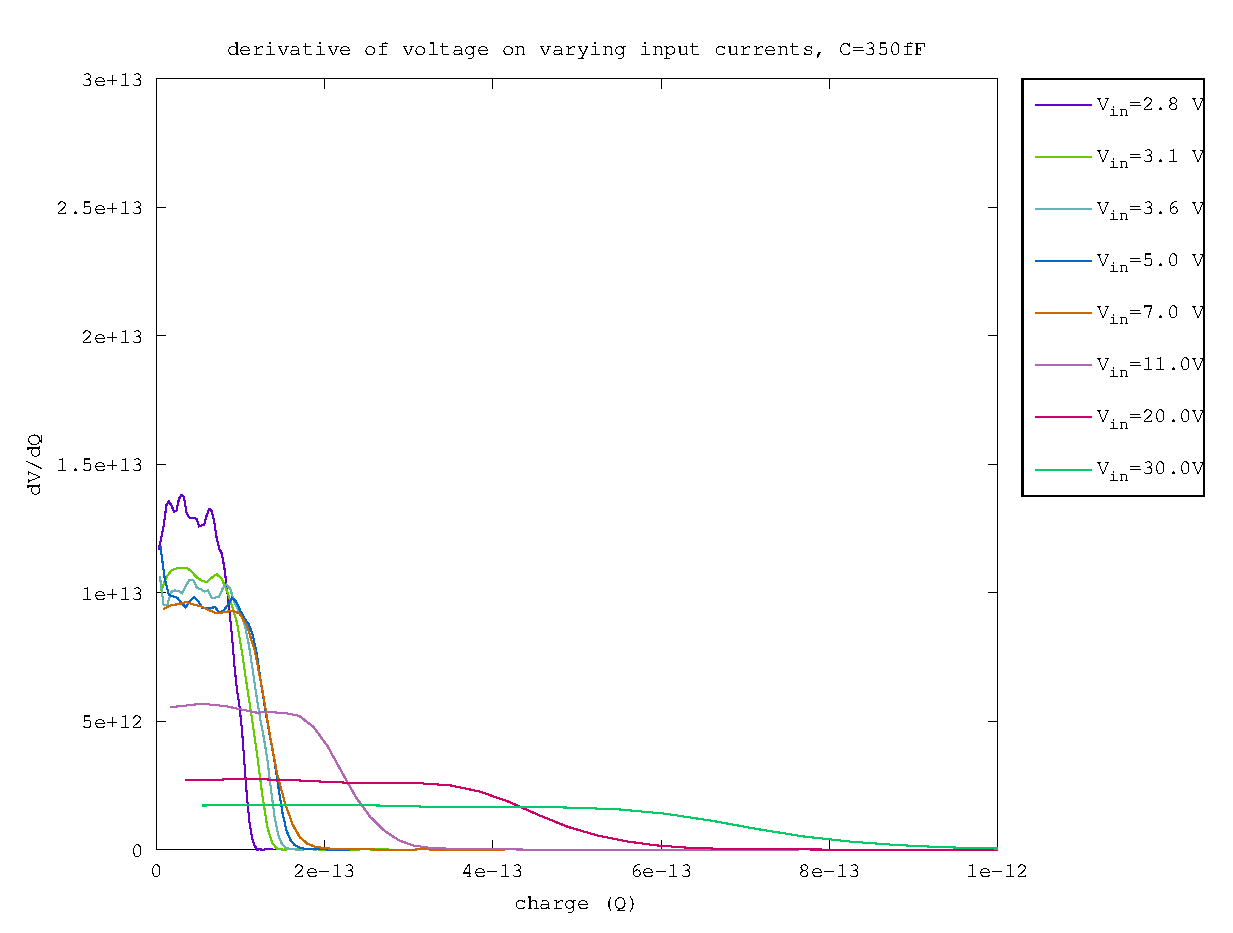
\includegraphics[width=\textwidth]{fig/bre_d_slope_350fF.eps}
        \caption {$C=350\,fF$}    
        \label{fig:bre_d_slopes_350fF}
    \end{subfigure}
    \vskip\baselineskip
    \begin{subfigure}[b]{0.475\textwidth}   
        \centering 
        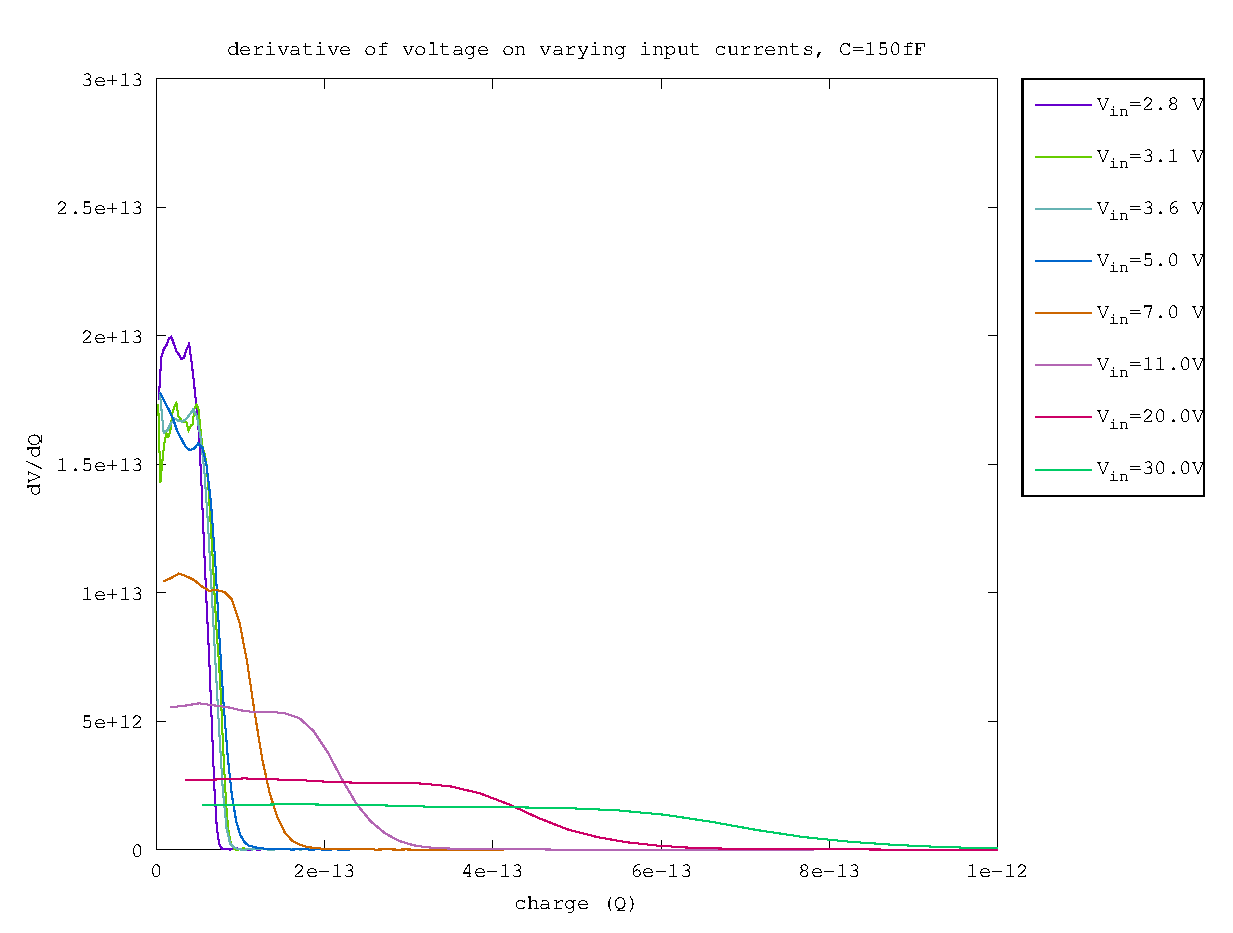
\includegraphics[width=\textwidth]{fig/bre_d_slope_150fF.eps}
        \caption {$C=150\,fF$}    
        \label{fig:bre_d_slopes_150fF}
    \end{subfigure}
    \quad
    \begin{subfigure}[b]{0.475\textwidth}   
        \centering 
        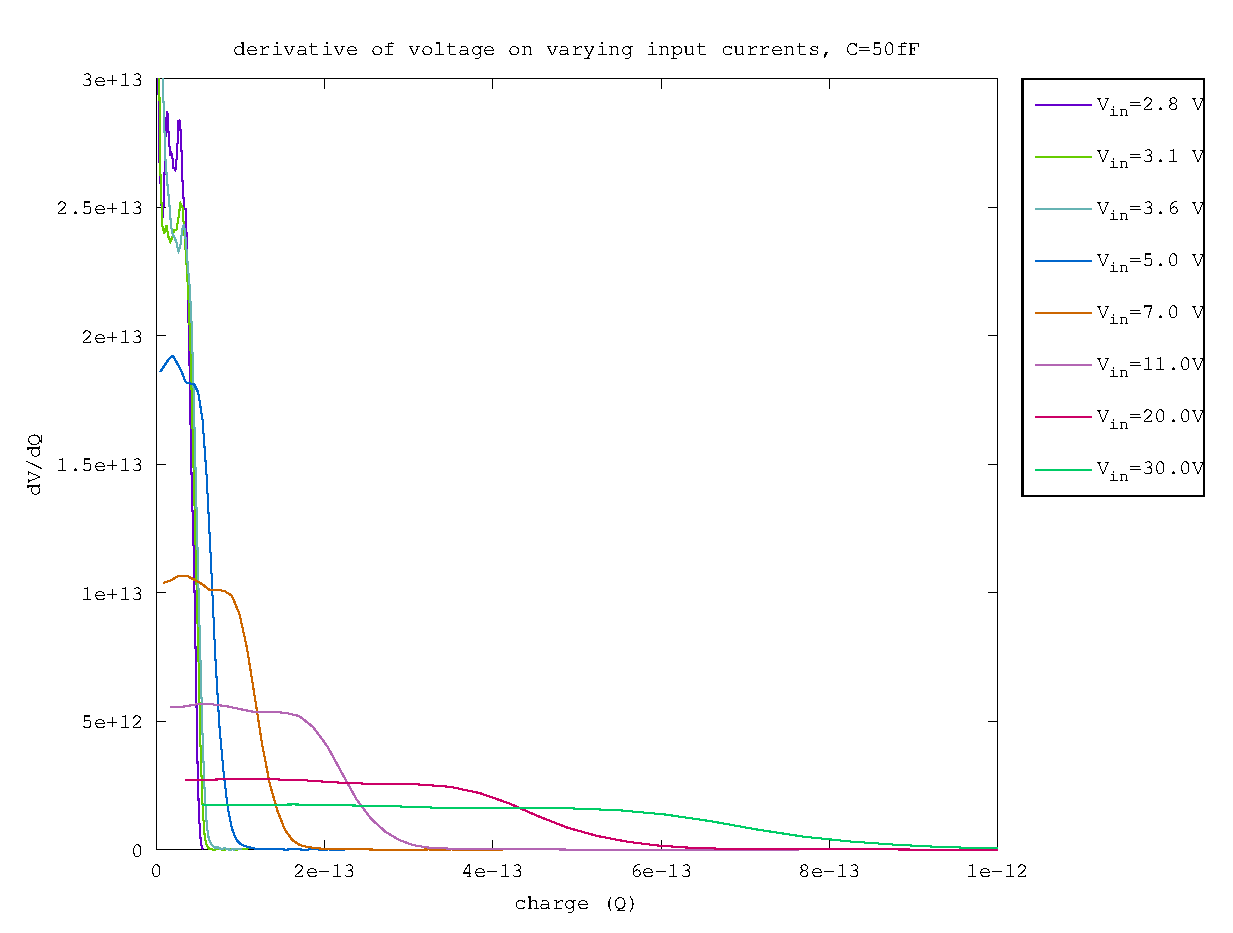
\includegraphics[width=\textwidth]{fig/bre_d_slope_50fF.eps}
        \caption{$C=50\,fF$}    
        \label{fig:bre_d_slopes_50fF}
    \end{subfigure}
    \caption{The plot shows dv/dt against time. The plot is in log scale, which allows for an easy read on the maximum slope and the time needed to discharge the integrator capacitance. }
    \label{fig:bre_d_slopes}
\end{figure}

\Cref{fig:bre_e_vs_m} shows the same plot as \cref{fig:e_vs_m}, but with higher current. This plot clearly shows that all four capacitance configurations saturate at a $\delta V\delta t \approx 3.1\,V$. This cannot be a limit applied to the input, because the capacitances are different. Therefore the output is limiting this, conform previous observations.

\begin{figure}[h]
    \centering
    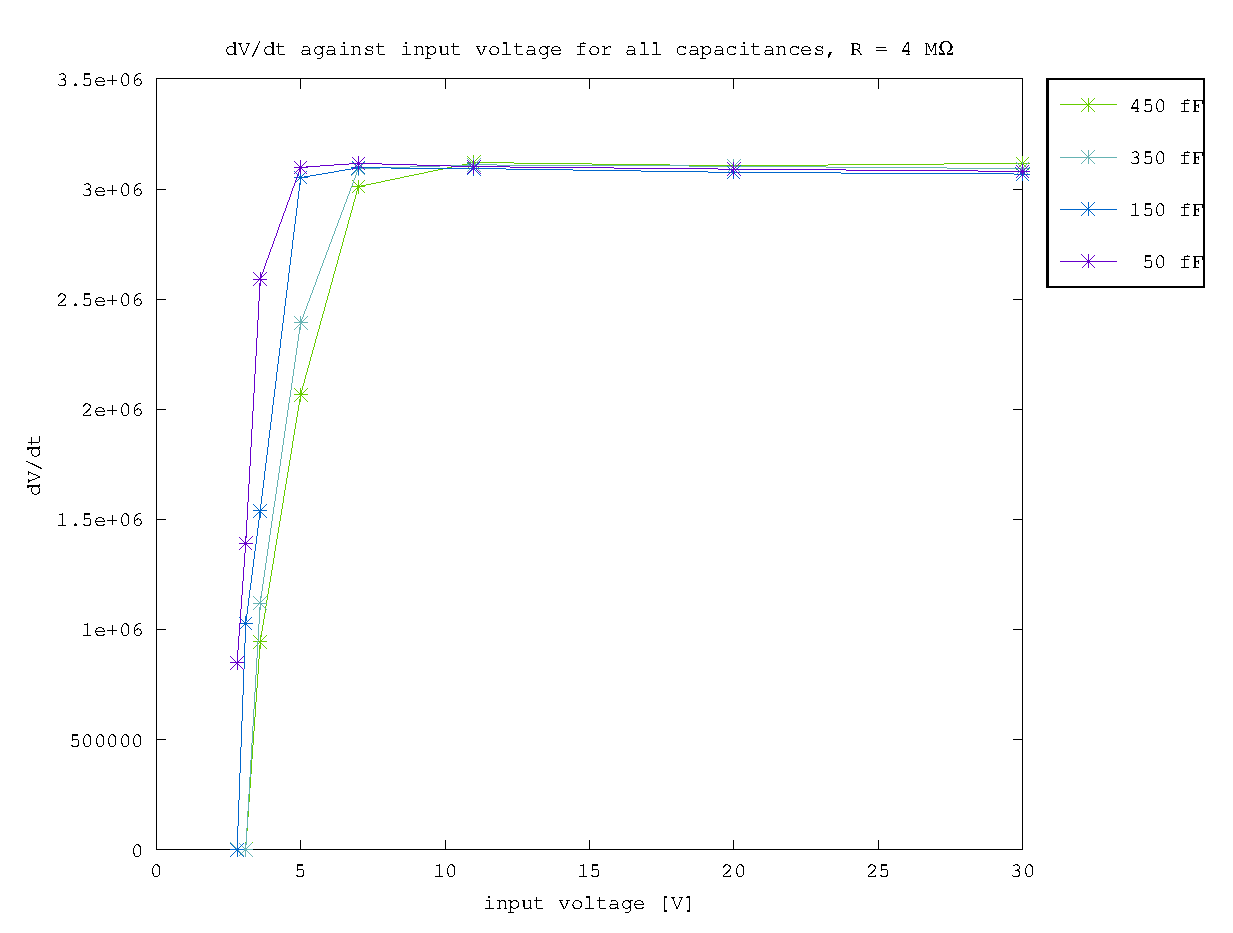
\includegraphics[width=\textwidth]{fig/bre_vin_vs_time_sat.eps}
    \caption {dV/dt against input voltage for all four capacitances. The x indicate the measurements.}    
    \label{fig:bre_e_vs_m}
\end{figure}

\clearpage
\subsubsection{VBO behavior}\label{sssec:VBO_behavior}


\subsection{Voltage limiter}\label{ssec:dynamic_voltage_limiter}



\section{GaN sensors with ROIC}\label{sec:GaN_sensors_with_ROIC}
After the ROIC is characterized with constant controlled current sources, the next step is to attach it to the GaN sensors. The target range of operating voltages for the GaN sensors is 0 to -$100\,V$. The primary interest lies in the I/V characteristics of the system. Because the same cations need to be performed all the time, it is worth to automate the setup one step further to save time.

\subsection{Setup}\label{ssec:GaN_setup}
In order to automate the measuring process further, the oscilloscope is connected to the laptop by cable, and directly controlled by \texttt{labVIEW}. \texttt{LabVIEW} automatically acquires the required waveforms from the oscilloscope, and calculates the slope in real time. This action is repeated and used to accumulate data points for the $I/V$ curve. When the  program is finished, the processed data is stored. A bashscript collects all the data and calls \texttt{octave-cli} to put the results in a plot. There are two ways, that have been used to controll the bias voltage of the GaN sensors. The first method is to use the arbitrary function generator (AFG) on the oscilloscope to generate a DC voltage between $-2.5$ and $2.5\,V$. A voltage amplifier with a gain of 10 is then used to achieve a range of $-25$ to $25\,V$ that is directly controllable in \texttt{labVIEW}. This allows \texttt{labVIEW} to automatically sweep the bias voltage. However, the range of $-25$ to $25\,V$ does not cover the target bias voltage range. Therefore, in order to increase the range further, a second method is used. This time the bias voltage is controlled manually with a voltage source. The oscilloscope measures both the input and output voltage. \texttt{LabVIEW} then calculates $x$ and $y$ co\"ordinates repeatedly. This method provides the operator with full control over which part of the $I/V$ curve is measured.

\subsection{Calculation of current}
The calculation of the current is done in labVIEW in realtime, and to accommodate for that, the calculation of the slope is different. First a voltage threshold , and a time threshold is set. Then it is calculated when the slope crosses either of those thresholds. That point is used together with the starting point to calculate the slope. Again in order to calculate the input current, the measurement is corrected for source follower, and the slope divided by the capacitance. 


\subsection{Automatic bias voltage sweep}\label{ssec:automatic_bias_voltage_sweep}
Measurements in this section are acquired using the automatic bias voltage sweep. First the performance in forward bias is investigated. The result of these measurements are shown in \cref{fig:pin26-40}. The VBO channel is used for the measurements because of the large currents. There are several oberservations that be made using this plot. First of all, there are several pins that appear to be unaffected by the input voltage. This is not due to the GaN sensors, but because the ROIC channel broke after a certain point. This is most likely because the input was accidently connected to a ground pin, which puts the high voltage directly to the input of the ROIC. A second observation is that the reset value of the VBO cannot be contained for large input voltages. This most likely means that the amount of current that is put into the ROIC is larger than the op amp in the ROIC can keep up with. Using an external current meter, the maximum amount of current the opamp can compete with is approximately $15\,\mu A$. Finally it is interesting to observe that there is a substantial variance across the different devices. In order to test whether this variance is due to noise or due to variance across devices, a second set of measurements are made. This time only a single device is measured. The results are shown in \cref{fig:pin32}. These measurements show that the variance over different measurements is relatively low, which means that the observed variance in \cref{fig:pin26-40} is mostly caused by variance across different devices.


\begin{figure}[h]
	\centering
	\begin{subfigure}[b]{0.475\textwidth}
	    \centering
	    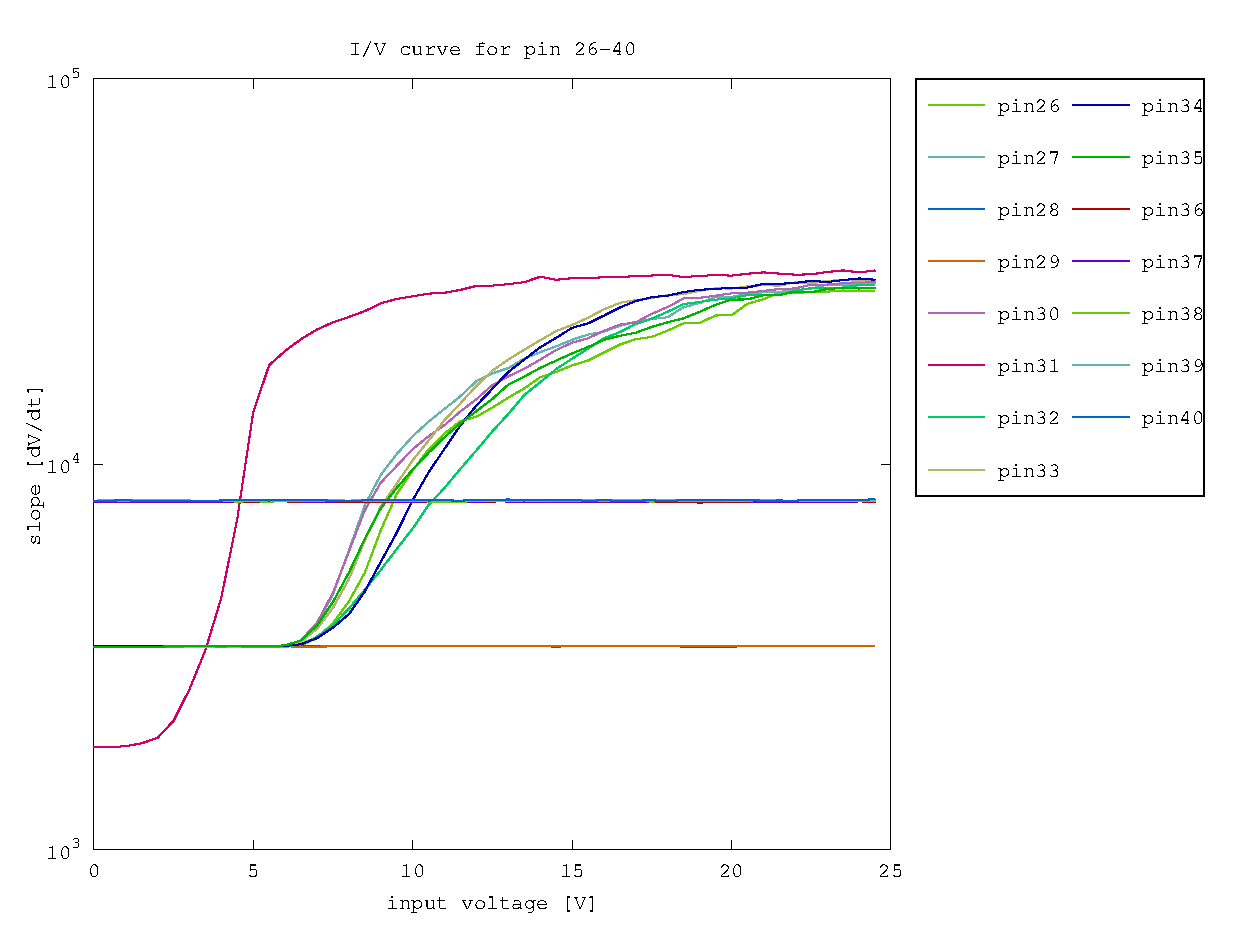
\includegraphics[width=\textwidth]{fig/pin26-40_slope_0-25V.eps}
	    \caption[Network2]%
	    {I/V characteristics}    
	    \label{fig:pin26-40_slope}
	\end{subfigure}
	\hfill
	\begin{subfigure}[b]{0.475\textwidth}  
	    \centering 
	    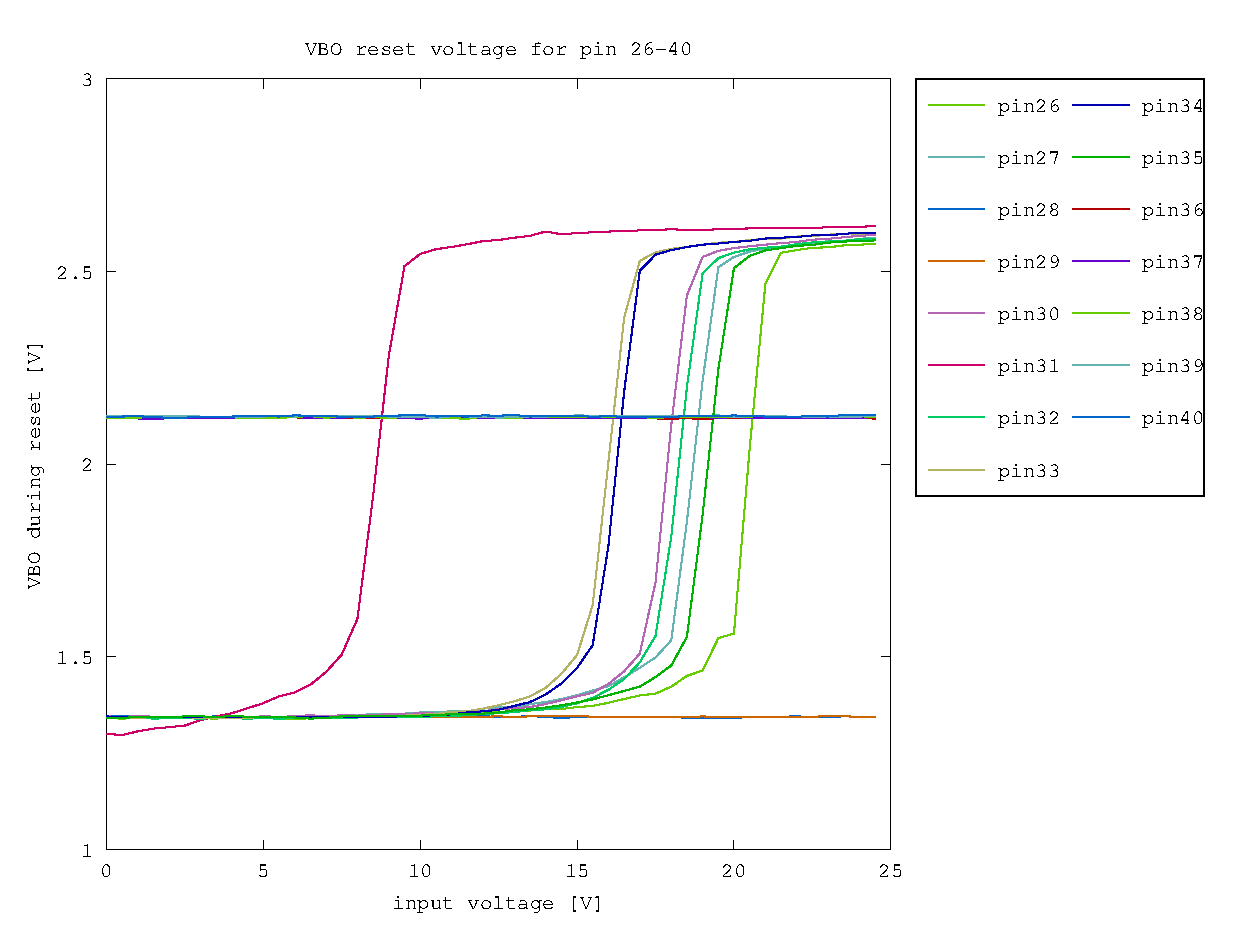
\includegraphics[width=\textwidth]{fig/pin26-40_reset_0-25V.eps}
	    \caption[]%
	    {reset value for VBO}    
	    \label{fig:pin26-40_reset}
	\end{subfigure}
	\caption{The slope and reset values for the VBO of pin26-40}
	\label{fig:pin26-40}
\end{figure}




\begin{figure}[h]
	\centering
	\begin{subfigure}[b]{0.475\textwidth}
	    \centering
	    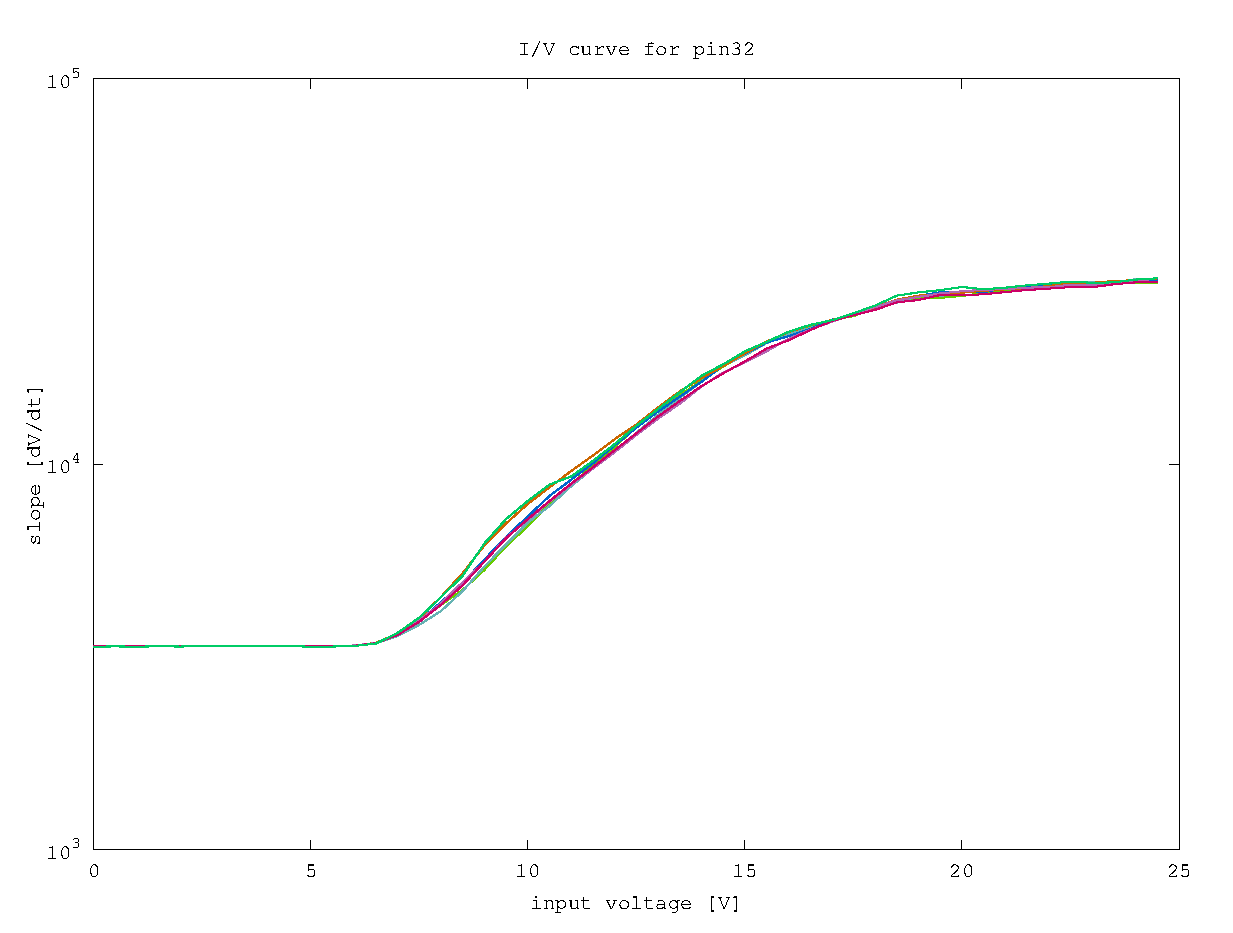
\includegraphics[width=\textwidth]{fig/pin32_slope_0-25V.eps}
	    \caption[Network2]%
	    {I/V characteristics}    
	    \label{fig:pin32_slope}
	\end{subfigure}
	\hfill
	\begin{subfigure}[b]{0.475\textwidth}  
	    \centering 
	    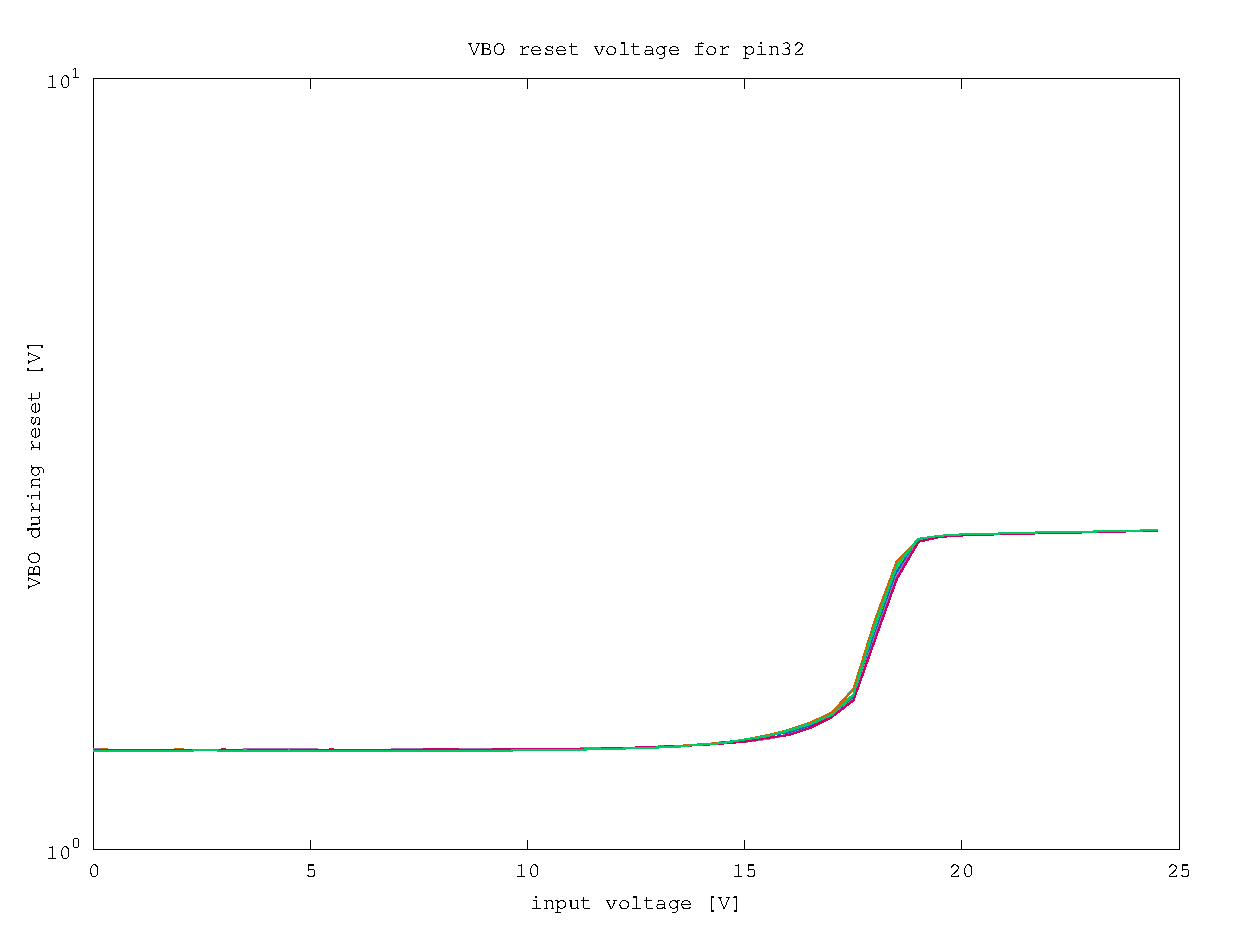
\includegraphics[width=\textwidth]{fig/pin32_reset_0-25V.eps}
	    \caption[]%
	    {reset value for VBO}    
	    \label{fig:pin32_reset}
	\end{subfigure}
	\caption{The slope and reset values for the VBO of pin32 repeated multiple times to test variance across measurements}
	\label{fig:pin32}
\end{figure}


Next, the reverse bias performance. The I/V characteristics for several pins are shown in \cref{fig:pin22_30_slope}. The jumps to negative current between 0 and $2.4\,V$ is due to the ground of the ROIC input being $2.4\,V$. Therefore for lower voltages, the current flows into the opposite direction. The numbers are not representative for the actual current though, because the ROIC and measurement method are not designed for that direction of current. The main observation that can be made is that the voltage range available in the current setup is insufficient to observe the most interesting part of the $I/V$ characteristics.  

\begin{figure}[h]
	    \centering
	    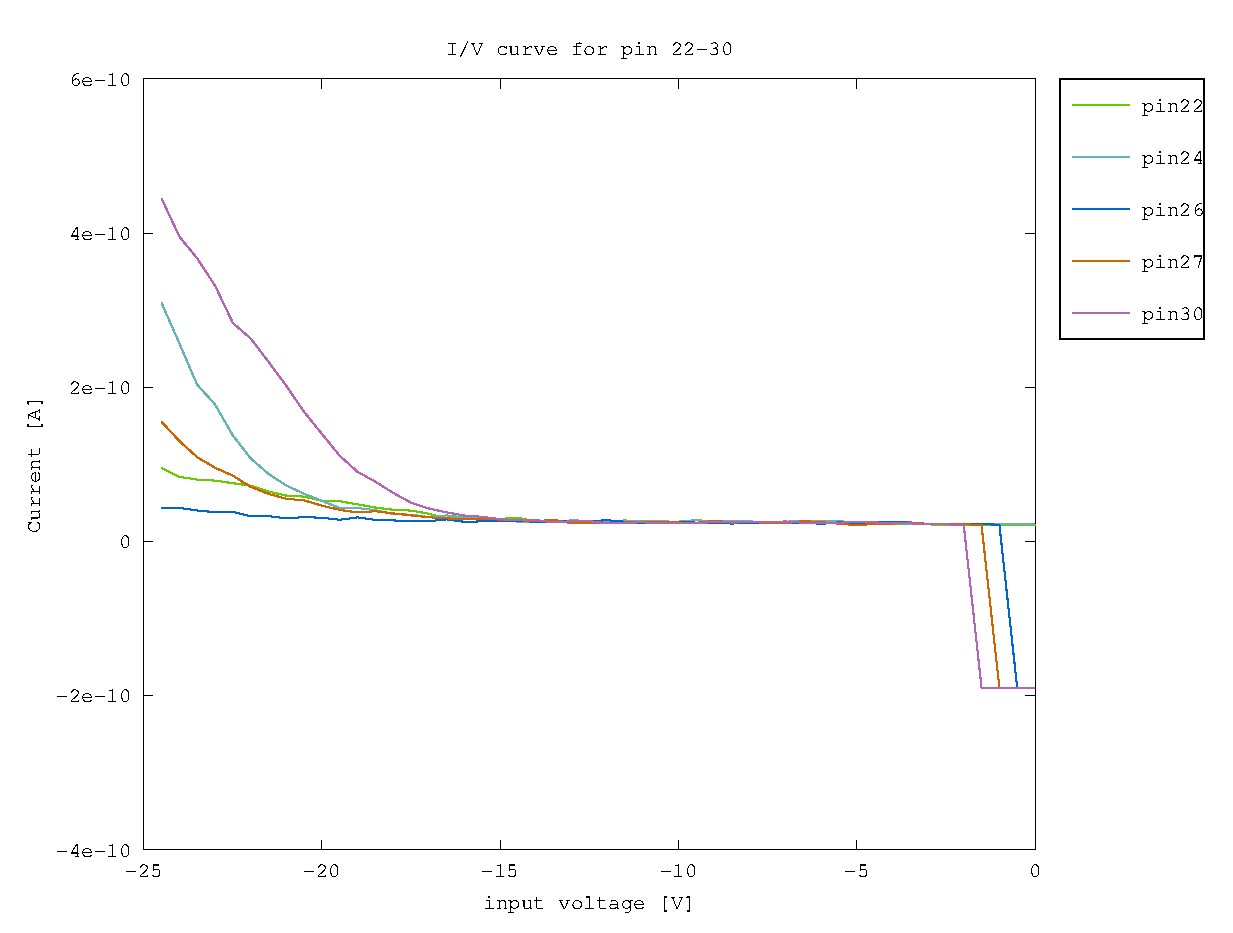
\includegraphics[width=0.8\textwidth]{fig/pin22-30_slope_-25-0V.eps}
	    \caption[]%
	    {Voltage to current characteristics for several GaN sensors}    
	    \label{fig:pin22_30_slope}	
\end{figure}  



\clearpage
\subsection{Manually controlled bias voltage}
To get to higher bias voltages, the bias voltages are manually controlled. This section will analyse measurement results based on individual sensors to determine both the GaN sensor and ROIc performance. 

The $I/V$ characteristics for pin 21 on the chip are shown in \cref{fig:pin21_slope}. Note that the pin number indicates the GaN sensor on a chip that is connected. The results in this plot match with the expected behavior of GaN sensors based on previous measurements. There is a small expontial increase in current for low bias voltages. At a high bias voltage the device goes into breakdown with a steep exponential increase.

\begin{figure}[H]
	    \centering
	    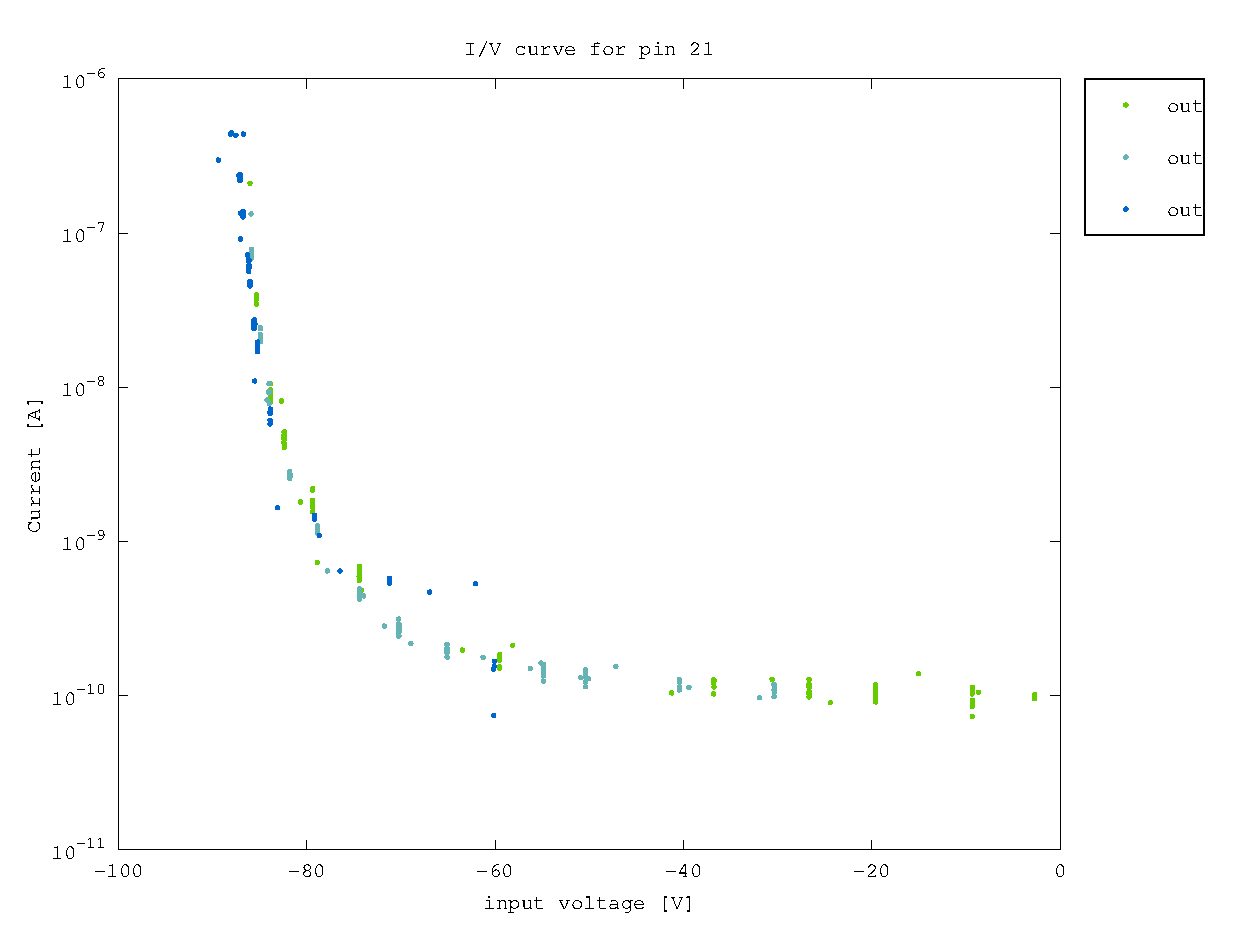
\includegraphics[width=0.7\textwidth]{fig/pin21_slope.eps}
	    \caption[]%
	    {Voltage to current characteristics for a single GaN sensor}    
	    \label{fig:pin21_slope}	
\end{figure}  

\Cref{fig:pin22_slope} shows a different behavior, with no change in the exponential slope. The flat area for very high bias voltages is due to the limit of the source follower. The reason for this might be that the breakdown voltage lies at a higher bias voltage than what can be observed with the current setup.

\begin{figure}[h]
	    \centering
	    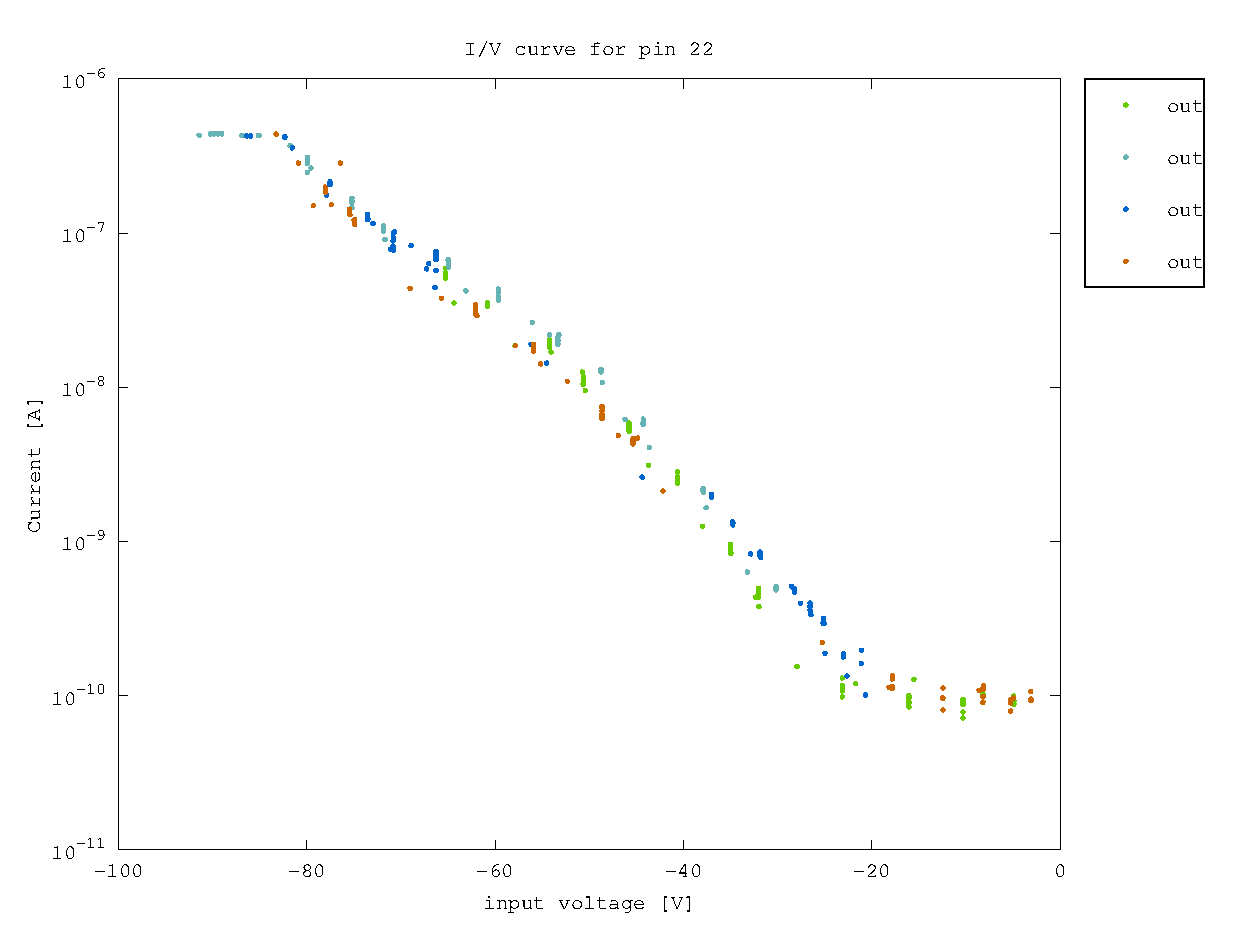
\includegraphics[width=0.7\textwidth]{fig/pin22_slope.eps}
	    \caption[]%
	    {Voltage to current characteristics for a single GaN sensor}    
	    \label{fig:pin22_slope}	
\end{figure}  


\Cref{fig:pin26_slope} shows the behavior of a different sensor. The behavior looks nothing like the previous observations which is most likely due to a defect in the sensor. The green OUT points can not rise to a higher value than approximately $380\,nA$. This limit is caused by the maximum slope on the source follower. In order to extend the reach of the ROIC further, the VBO is used. As concluded in \cref{sssec:VBO_behavior}, the VBO can handle higher voltages because of the higher capacitance. Combining VBO and OUT therefore allows for a large dynamic range. 

\begin{figure}[h]
	    \centering
	    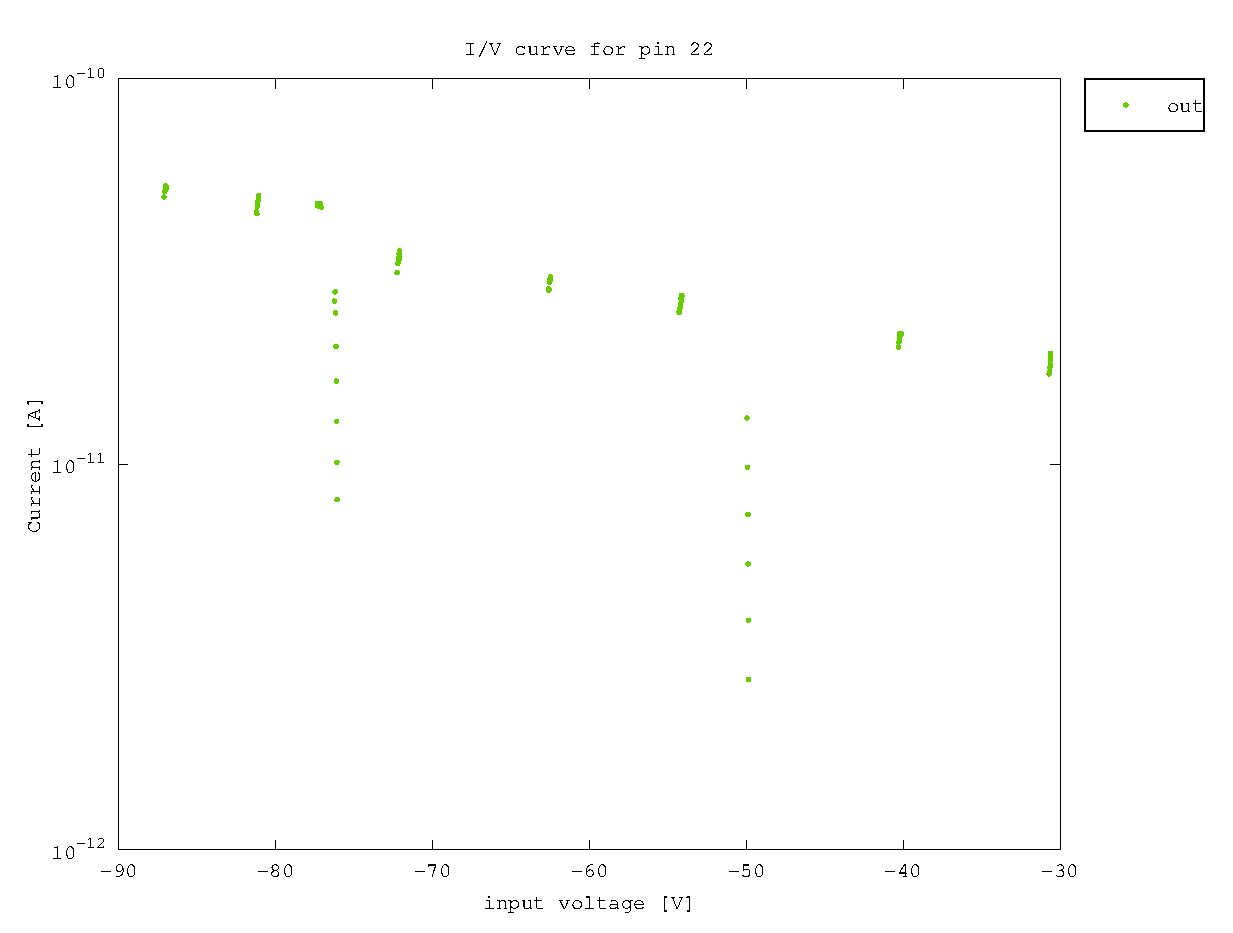
\includegraphics[width=0.7\textwidth]{fig/pin26_slope.eps}
	    \caption[]%
	    {Voltage to current characteristics for a single GaN sensor}    
	    \label{fig:pin26_slope}	
\end{figure}  

\Cref{fig:pin18_slope} and \cref{fig:pin18_slope_lin} show plots for a sensor that is illuminated by a UV source. One can see that the dark current has a steeper slope than the UV light. This means that a clear difference is oberservable for low bias voltages, but the UV loses significance when the dark current increases to higher levels.

\begin{figure}[h]
	    \centering
        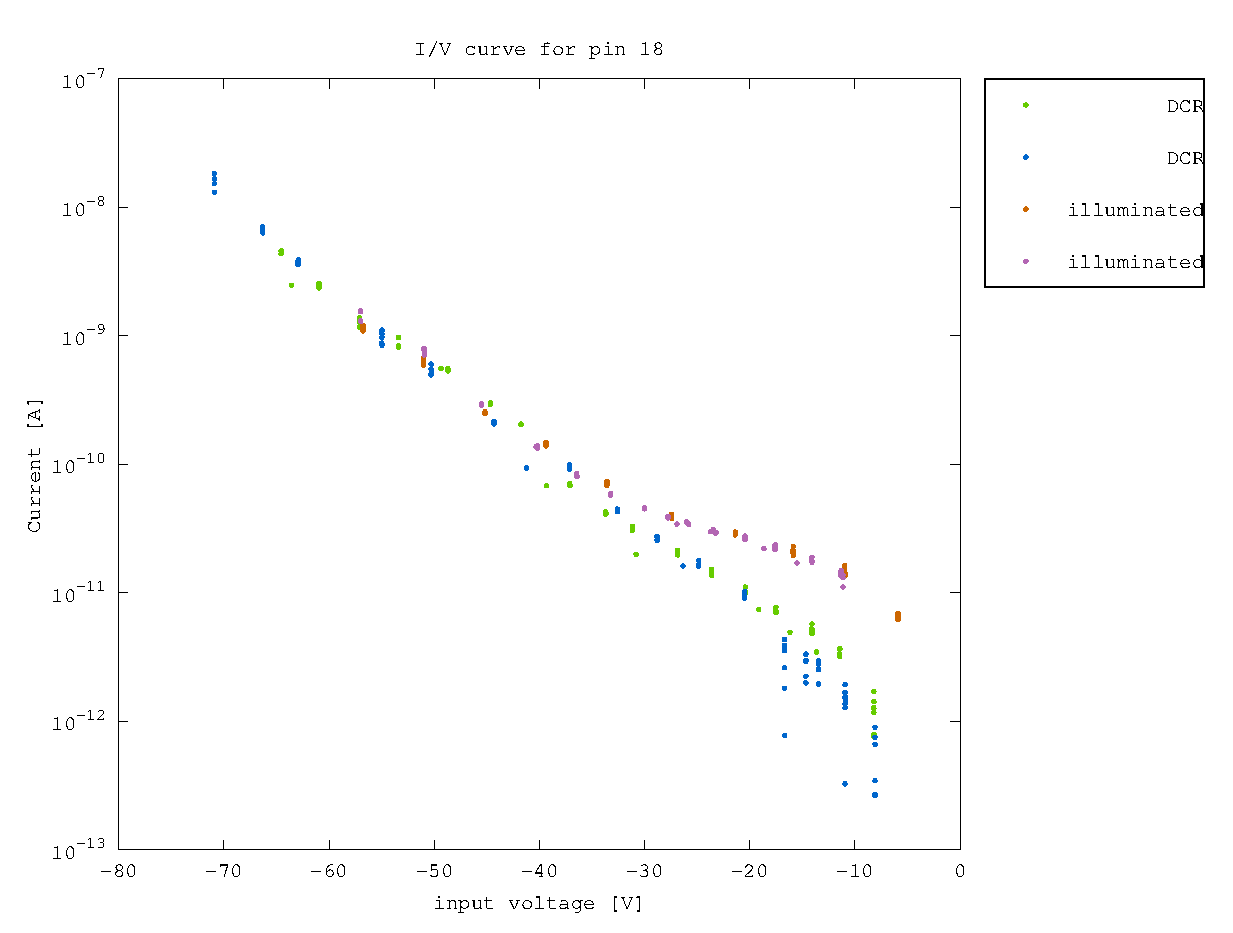
\includegraphics[width=0.7\textwidth]{fig/pin18_slope_UV.eps}
	    \caption[]%
	    {Voltage to current characteristics for a single GaN sensor}    
	    \label{fig:pin18_slope}	
\end{figure}  

\begin{figure}[h]
	    \centering
        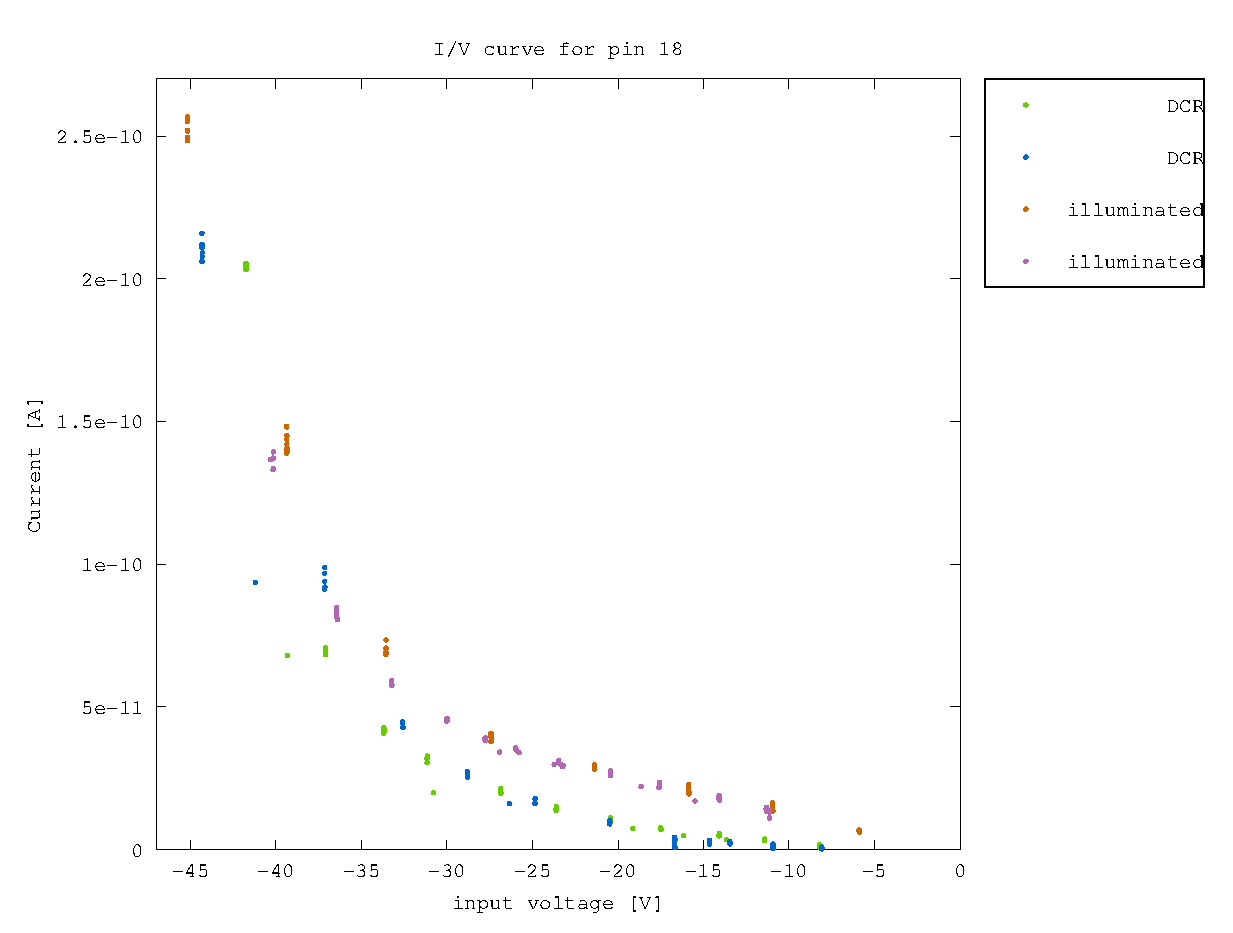
\includegraphics[width=0.7\textwidth]{fig/pin18_slope_lin_UV.eps}
	    \caption[]%
	    {Voltage to current characteristics for a single GaN sensor}    
	    \label{fig:pin18_slope_lin}	
\end{figure}  

\clearpage
\subsection{Very high bias voltage}\label{ssec:very_high_bias_voltage}
Besides the $I/V$ measurements, a second observation was made. Specifically, the performance of the ROIC with the GaN sensors for very high bias voltages between 90 and $100\,V$. When the amount of current reaches a certain level, the ROIC is no longer able to maintain it's reset values. This means that during reset, the op amp inside the RIOC is not able to keep up with current produced in the GaN sensor. This causes the input of the integrator to rise to the point that the voltage limiter kicks in. There are two things happening here. This means that the ROIC is no longer functioning. There is a second more problematic effect however. When this modus is kept for to long and/or at a voltage that is too high, the ROIC creates a spark. After that the ROIC is no longer useable. Because of this, three ROICs where damaged. A photo of the inside of the three packaged chips is shown in \cref{fig:burned_chips}. The burns on the chips are on different wires, but for all chips, the burned wire is is the input of the channel that was used at that time. For all three cases, did the wirebond melt and disconnect. However, this is most likely a secondary effect. Especially because the entire chip stops functioning, which should not be the case if only the wirebond fails. Another observation is that the VBO output is pulled to ground, which means that the input is most likely shorted to ground. 


\begin{figure}[H]
	    \centering
	    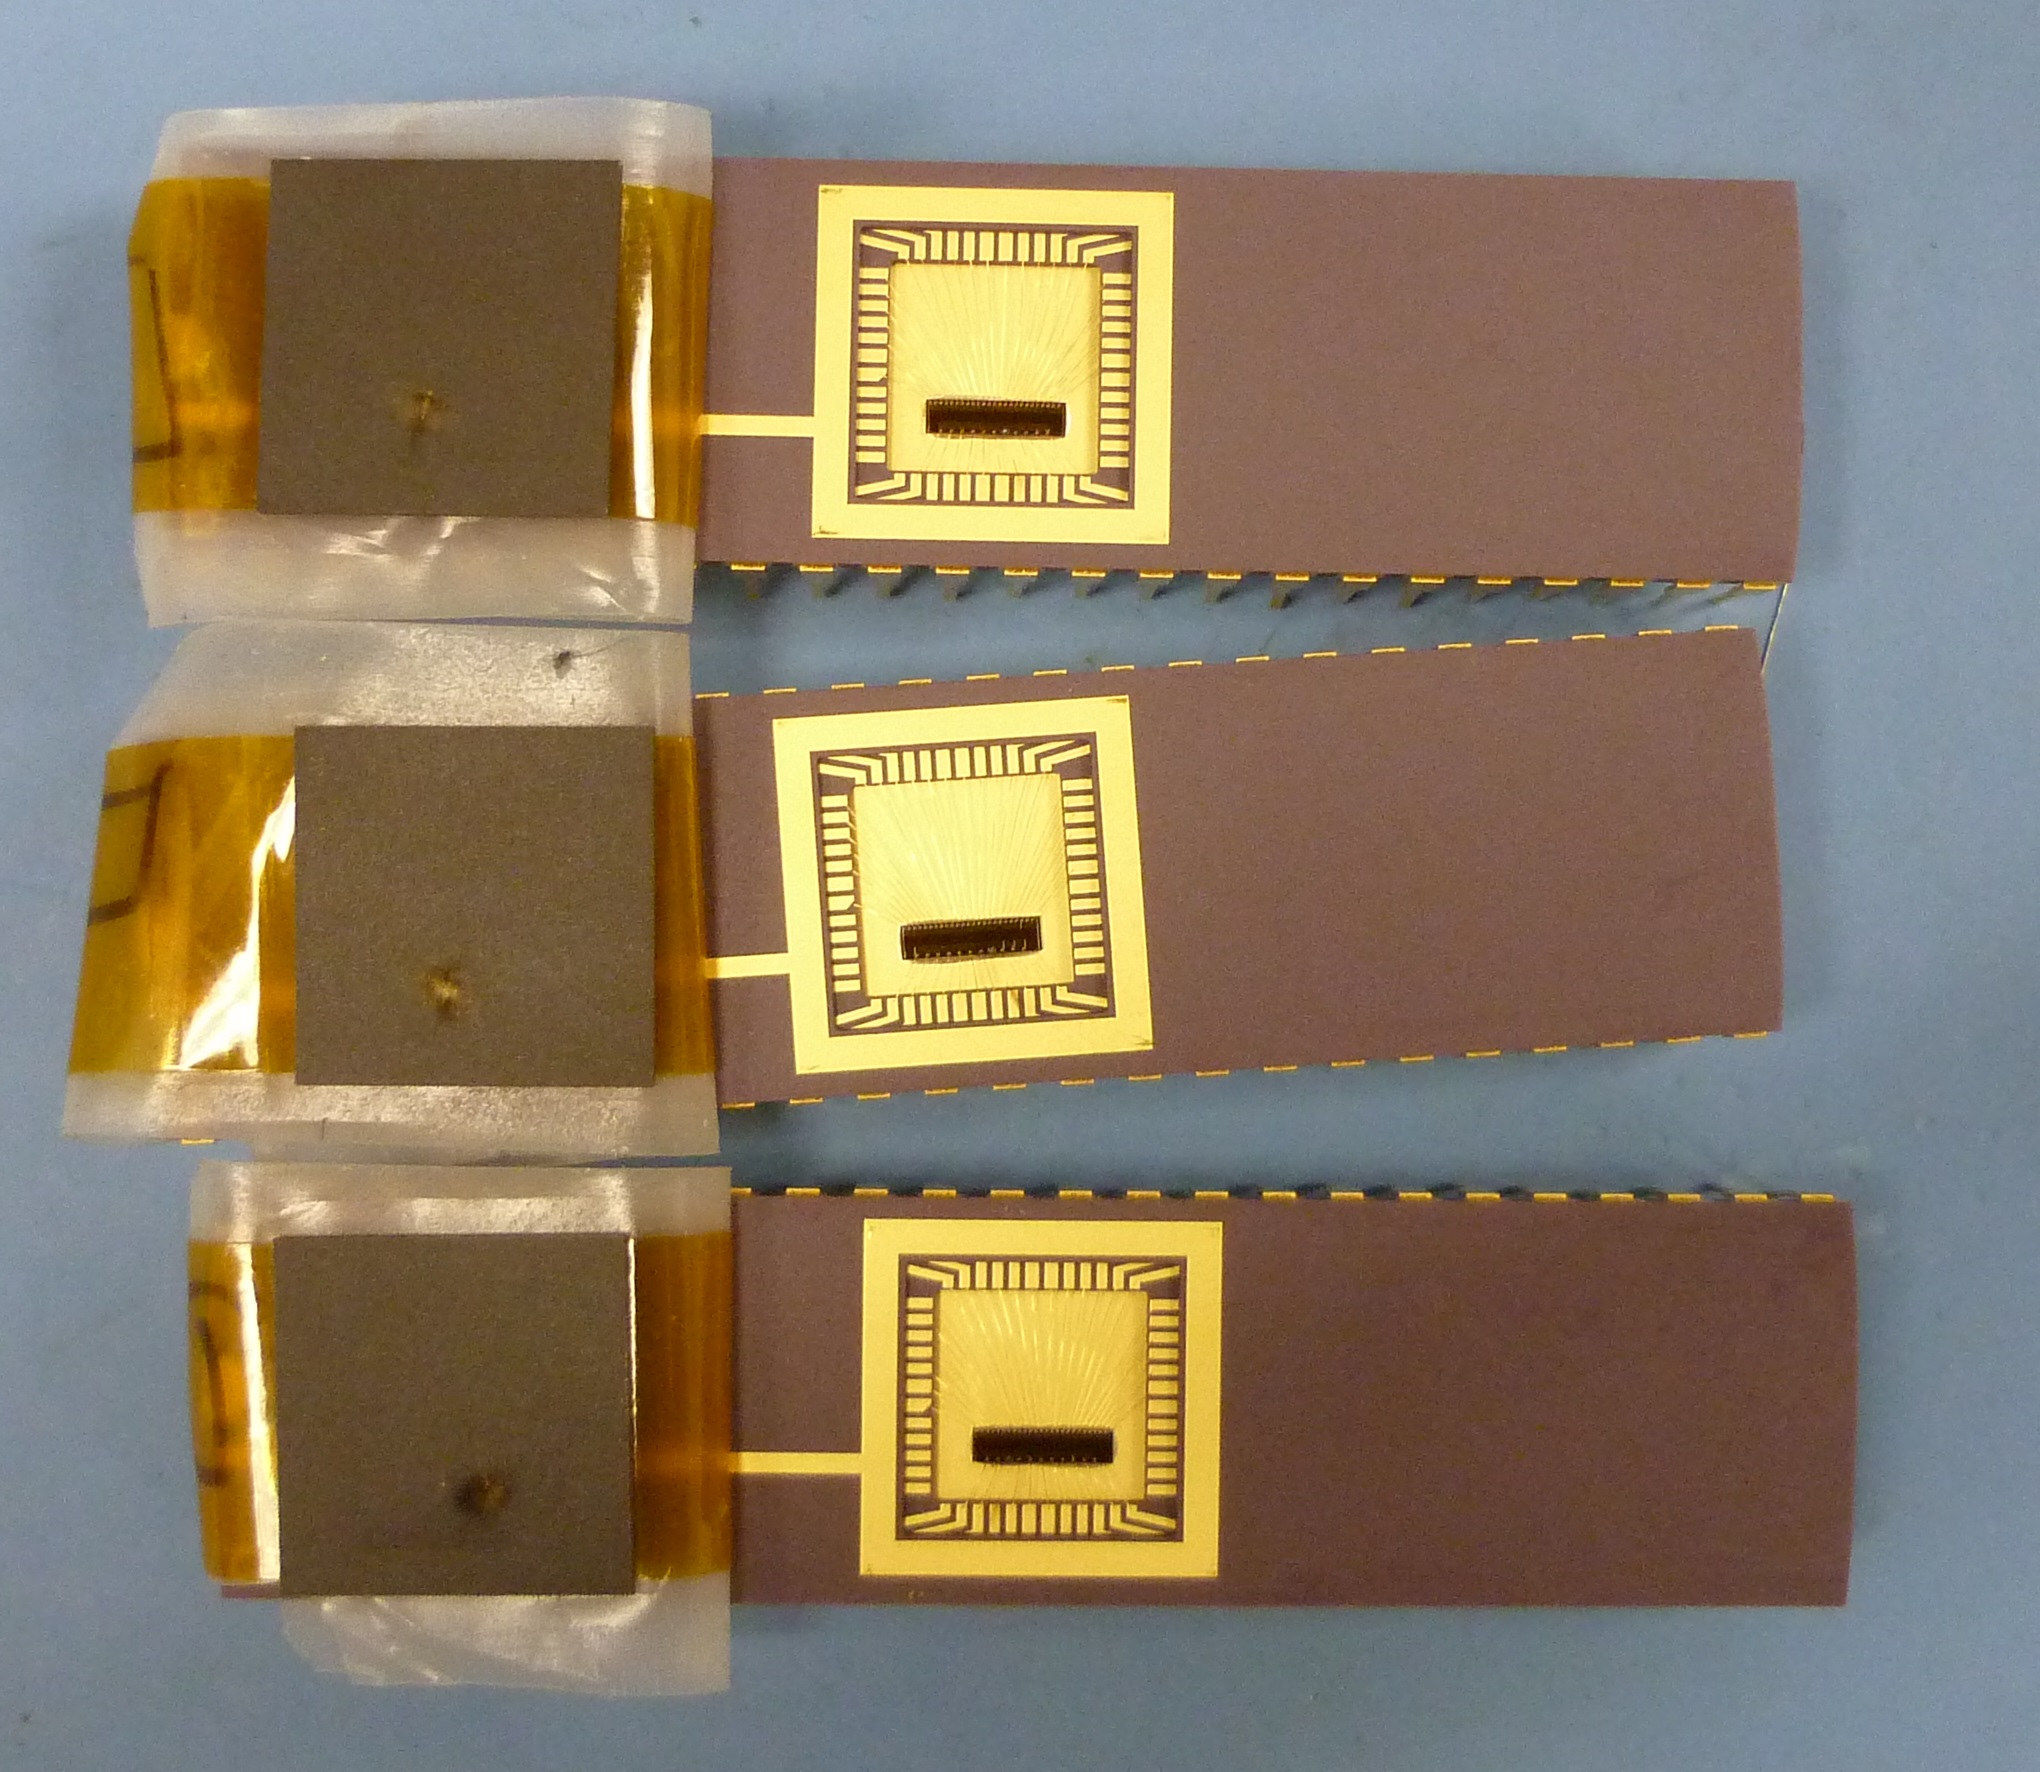
\includegraphics[width=0.7\textwidth]{fig/burned_chips.JPG}
	    \caption[]%
	    {Inside of packaged ROIC chips after being exposed to too much power}    
	    \label{fig:burned_chips}	
\end{figure}  

This effect is currently the largest constraint to measuring the GaN sensors at high bias voltages, because the ROIC dies before the GaN sensors do.


\section{Conclusions and Future work}\label{sec:conclusions_and_future_work}



\appendix
%\section{setup}\label{sec:setup}
\begin{figure}[H]
\centering
\usetikzlibrary{shapes,snakes}
\tikzstyle{dot} = [draw,shape=circle,fill=black, scale =.2]
\tikzstyle{l_arrow} = [draw,fill = black, regular polygon,regular polygon sides=3, rotate=-90, anchor=south, scale=.5] 
\tikzstyle{l_text} = [anchor=south west]
\tikzstyle{r_arrow} = [draw,fill = black, regular polygon,regular polygon sides=3, rotate=90, anchor=south, scale=.5] 
\tikzstyle{r_text} = [anchor=south east]
\begin{tikzpicture}[scale=1.5, every node/.style={scale=1}]


\node[l_text] at (-3,1) {VDD 3.3 (1)};
\node[l_text] at (-3,0) {IN[8] (15)};
\node[l_text] at (-3,-1) {VSUB (16)};
\node[l_text] at (-3,-2) {VDD\_HV (17)};
\node[l_text] at (-3,-3) {GND\_HV (18)};

\node[l_arrow] at (-3,1) {};
\node[l_arrow] at (-3,0) {};
\node[l_arrow] at (-3,-1) {};
\node[l_arrow] at (-3,-2) {};
\node[l_arrow] at (-3,-3) {};

\node[r_text] at (0,1) {(25) gnd};
\node[r_text] at (0,0) {(26) VDD5};
\node[r_text] at (0,-1) {(27) Vg};
\node[r_text] at (0,-2) {(28) Rst[3]};
\node[r_text] at (0,-3) {(29) Rst[1]};
\node[r_text] at (0,-4) {(30) Rst[2]};
\node[r_text] at (0,-5) {(31) Res};
\node[r_text] at (0,-6) {(32) VB0[8]};
\node[r_text] at (0,-7) {(33) out[8]};
\node[r_text] at (0,-8) {(48) gnd};


\node[r_arrow] at (0,1) {};
\node[r_arrow] at (0,0) {};
\node[r_arrow] at (0,-1) {};
\node[r_arrow] at (0,-2) {};
\node[r_arrow] at (0,-3) {};
\node[r_arrow] at (0,-4) {};
\node[r_arrow] at (0,-5) {};
\node[r_arrow] at (0,-6) {};
\node[r_arrow] at (0,-7) {};
\node[r_arrow] at (0,-8) {};
\draw  (-3,2) rectangle (0,-8);




\draw (-3.5,-1) node[ground]{} to (-3,-1);
\draw (-3.5,-3) node[ground]{} to (-3,-3);
\draw (0.5,1) node[ground]{} to (0,1);
\draw (0.5,-8) node[ground]{} to (0,-8);
\draw (0.5,-3) node[ground]{} to (0,-3);
\draw (0.5,-4) node[ground]{} to (0,-4);

\draw (0.5,0.25) node[anchor=south]{$5\,V$} (0.5,0.25) node[tground]{} to (0.5,0)to (0,0); % VDD5
\draw (0.5,-0.75) node[anchor=south]{$4.5\,V$} (0.5,-0.75) node[tground]{} to (0.5,-1)to (0,-1); % Vg
\draw (-3.5,1.25) node[anchor=south]{$3.3\,V$} (-3.5,1.25) node[tground]{} to (-3.5,1)to (-3,1); % VDD3.3
\draw (-3.5,-1.75) node[anchor=south]{$5\,V$} (-3.5,-1.75) node[tground]{} to (-3.5,-2)to (-3,-2); %VDD_HV
\draw (-4.5,0.25) node[anchor=south]{$set$} (-4.5,0.25) node[tground]{} to (-4.5,0)to (-4.5,0); % IN[8]
\draw (0.5,-1.75) node[anchor=south]{$reset$} (0.5,-1.75) node[tground]{} to (0.5,-2)to (0,-2); % Rst[3]
\draw  (0,-5) to[R=$50\,k\Omega$](1.5,-5) to (1.5,-4.75) node[tground]{} (1.5,-4.75) node[anchor=south]{$5\,V$}; %res


\draw (-4.5,0) to [R=$20\,M\Omega$](-3,0);

\end{tikzpicture}
\caption{Schematic of breadbord}
\label{tkz:breadbord}
\end{figure}
\begin{figure}[H]
\centering
\usetikzlibrary{shapes,snakes}
\tikzstyle{dot} = [draw,shape=circle,fill=black, scale =.3]
\tikzstyle{l_arrow} = [draw,fill = black, regular polygon,regular polygon sides=3, rotate=-90, anchor=south, scale=.5] 
\tikzstyle{l_text} = [anchor=south west]
\tikzstyle{r_arrow} = [draw,fill = black, regular polygon,regular polygon sides=3, rotate=90, anchor=south, scale=.5] 
\tikzstyle{r_text} = [anchor=south east]
\begin{tikzpicture}[scale=1, every node/.style={scale=1}]

\draw[dashed, color=blue]  (-0.5,5.5) rectangle (0.5,-2);
\fill[color=blue, opacity=.1]  (-0.5,5.5) rectangle (0.5,-2);
\node[align=center, anchor=south] at (0,5.5) {voltage\\limiter};

\draw[dashed, color=green]  (1.25,5.5) rectangle (5.25,-2);
\fill[opacity=.1, color=green]  (1.25,5.5) rectangle (5.25,-2);
\node[align=center, anchor=south] at (3.25,5.5) {integrator};



\draw[dashed, color=red]  (5.75,5.5) rectangle (9.25,-2);
\fill[opacity=.1, color=red] (5.75,5.5) rectangle (9.25,-2);
\node[align=center, anchor=south] at (7.5,5.5) {current mirrors};

%\draw (0,0) to node[nfet]{};

%\draw (0,0) to (mos1.s);
\node(Vg)[nfet, rotate=-90] at (0,2.5) {};
\node[nfet, rotate=-90] (Reset) at (2.5,2) {};
\node[pfet] (CM_H1) at (5,3) {};
\node[nfet] (CM_L1) at (5,-1) {};
\node[nfet] (CM_H2) at (7,3) {};
\node[nfet] (CM_L2) at (7,-1) {};
\node[nfet] (CM_H3) at (9,3) {};
\node[nfet] (CM_L3) at (9,-1) {};



\draw (-1,2.5) node[anchor=east]{IN[i]} to (Vg.S);
\draw (Vg.G) |- (0,4.5) node[anchor=south]{Vg};
\draw (Vg.B) |- (1,2.5) node[dot]{} |- (CM_H1.G); %top
\draw (1,2.5) |- (1,0.5)  to [C=$450\,fF$](4,0.5) -| (CM_H1.D);
\draw (1.5,0.5) node[dot]{} -| (1.5,2) |- (Reset.B);
\draw (Reset.G) to (2.5,4.5) node[anchor=south]{Rst[3]};
\draw (Reset.D) -| (3.5,0.5) node[dot]{};
\draw (5,0.5) node[dot]{} to (CM_L1.D);
\draw (CM_L1.G) to (4,4.5) node[anchor=south]{Res}; 
\draw (CM_L1.S) to (CM_L2.S) to (7,-2.5) node[anchor=north]{gnd};
\draw (CM_H1.B) |- (CM_H2.D) to (7,4.5) node[anchor=south]{VDD3.3};
\draw (CM_L2.G) |- (4,0) node[dot]{};
\draw (5,0.5) -| (CM_H2.G);
\draw (CM_L1.B) to (CM_L1.S);
\draw (CM_L2.B) to (CM_L2.S);
\draw (CM_H2.B) to (CM_L2.D);
\draw (CM_H3.B) to (CM_L3.D);
\draw (1,3)node[dot]{} |- (8,4) |- (CM_H3.G);
\draw (CM_H3.D) |- (CM_H2.D) node[dot]{};
\draw (CM_L3.S) |- (CM_L2.S) node[dot]{};
\draw (CM_L3.G) |- (6,0) node[dot]{};
\draw (7,1.5)node[dot]{} to (10,1.5) node[anchor=west]{OUT[i]};
\draw (9,1)node[dot]{} to (10,1) node[anchor=west]{VBO[i]};



\end{tikzpicture}\caption{Schematic of ROIC channel}
\label{tkz:schematic_ROIC}
\end{figure}


\begin{figure}[h]
	\centering
	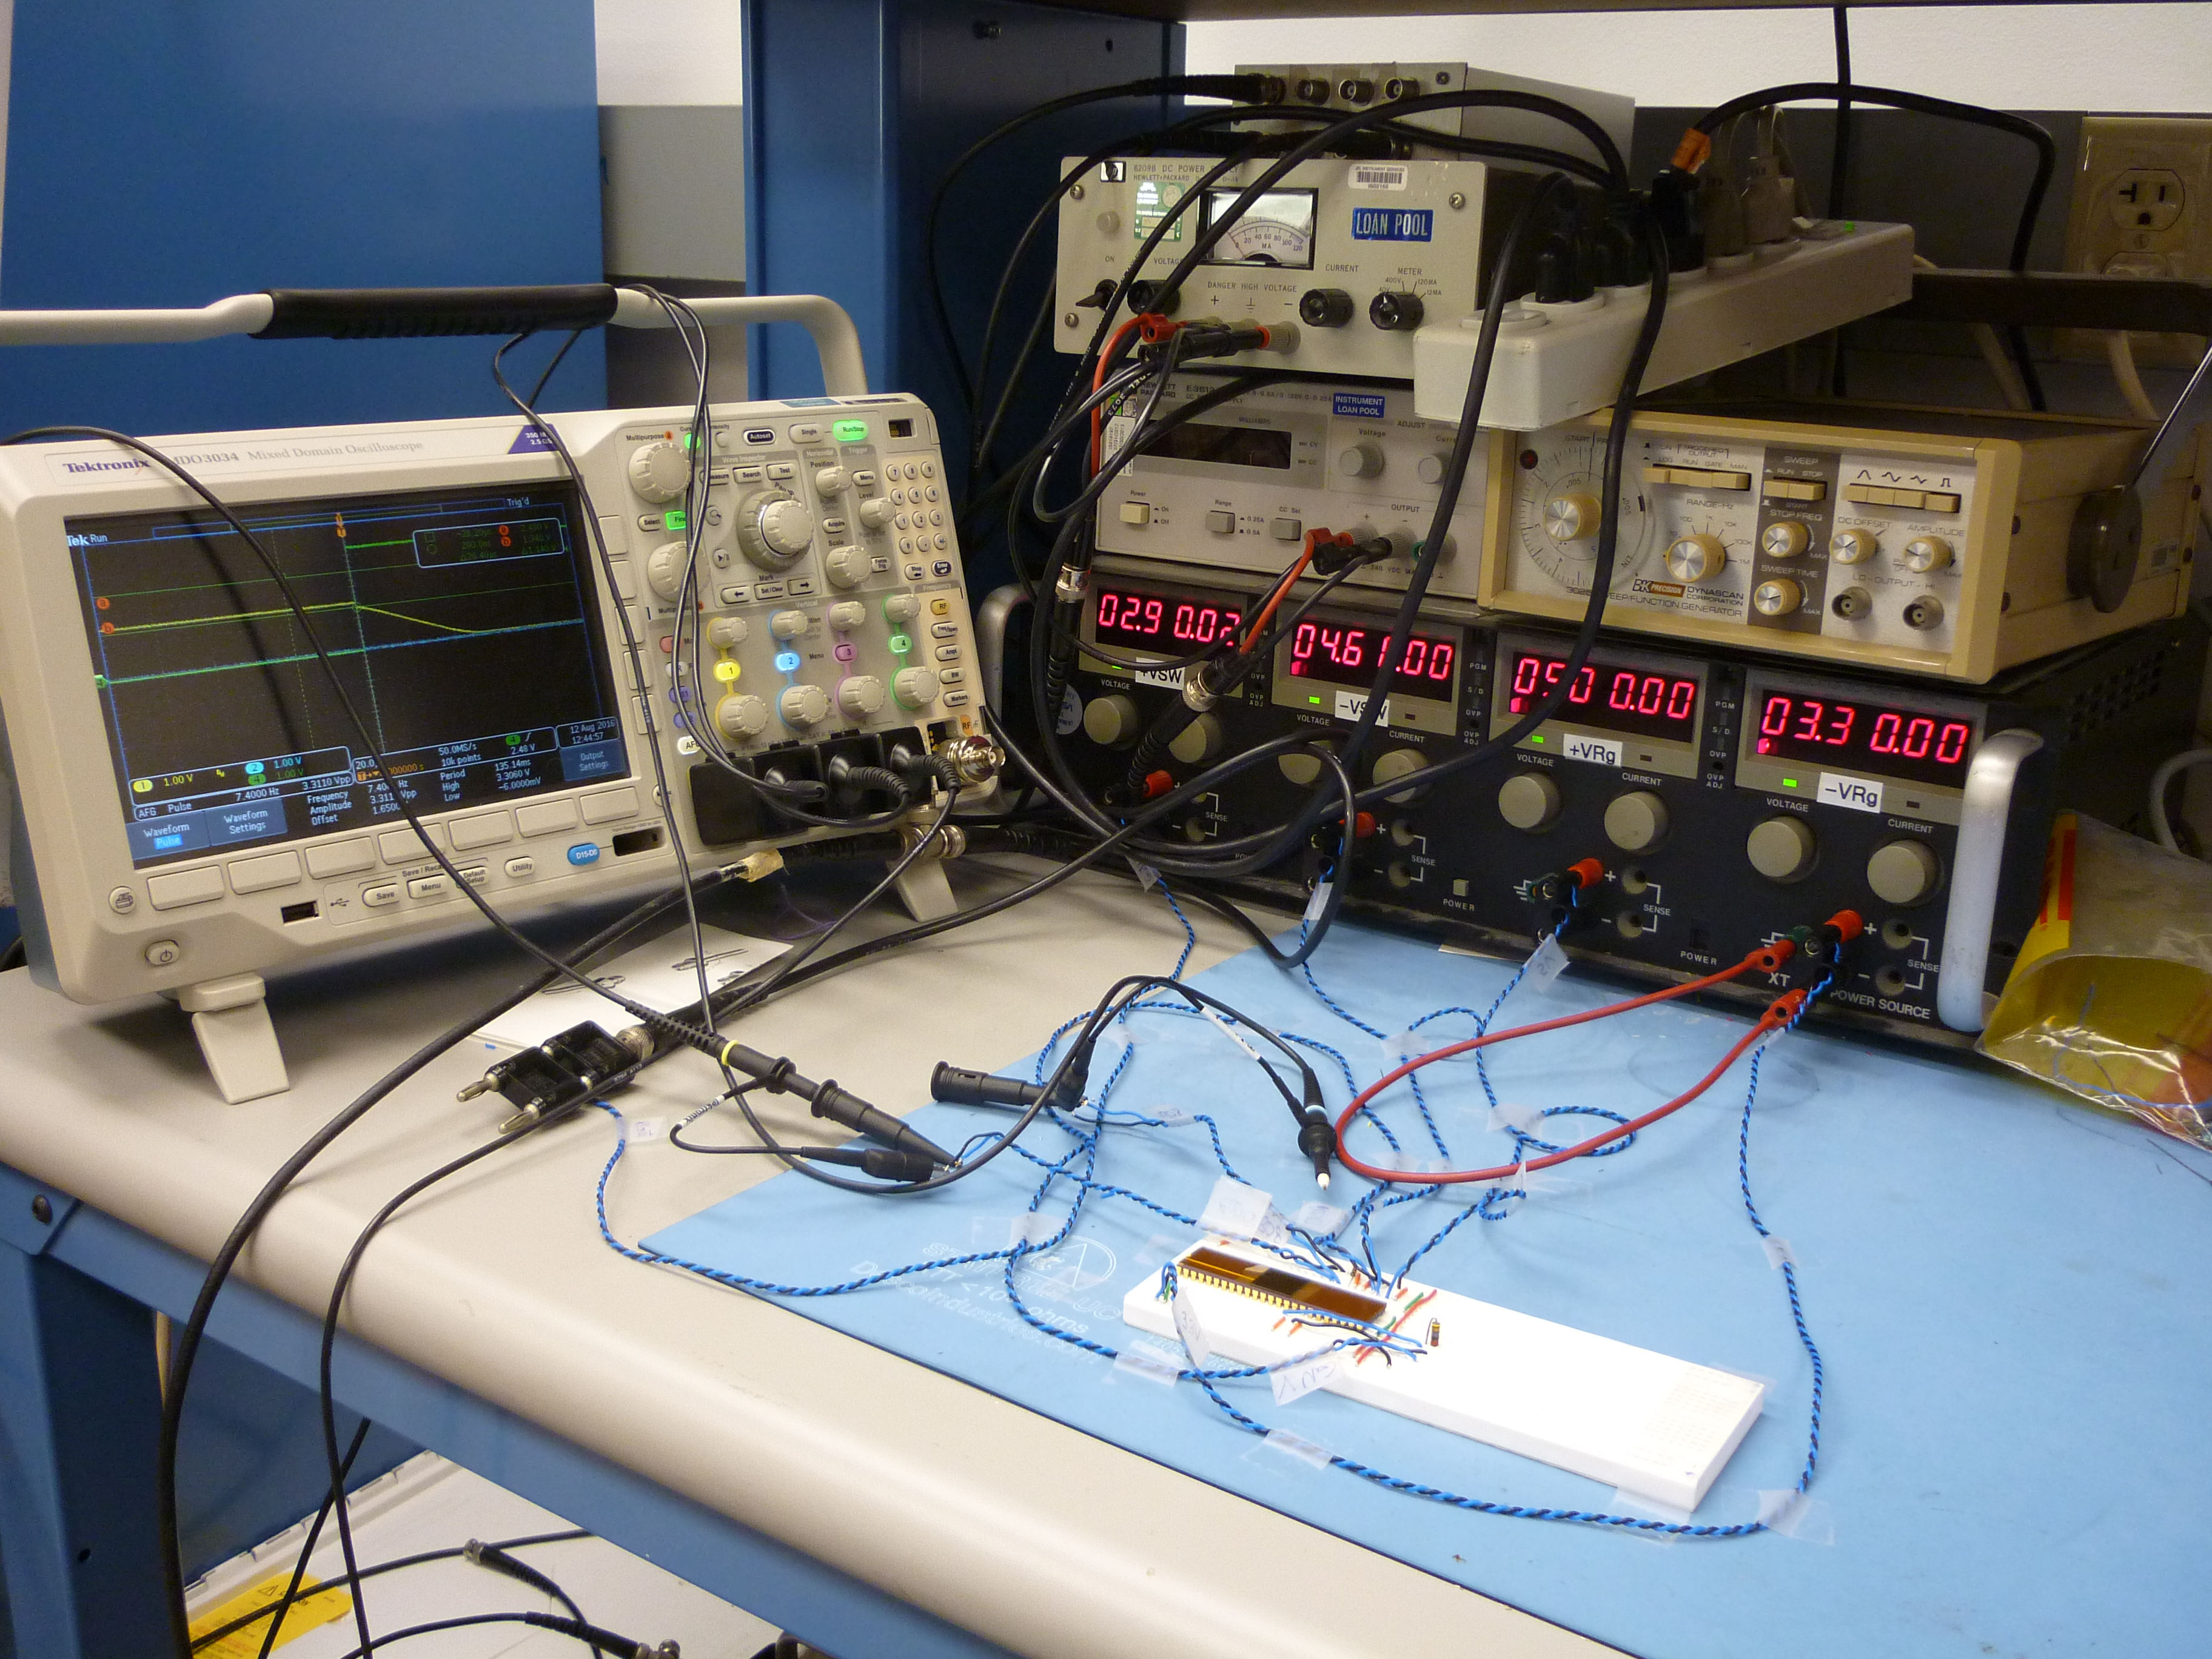
\includegraphics[width=0.6\linewidth]{fig/P1010158.JPG}
	\caption{setup overview}
	\label{fig:setup_overview}
\end{figure}

\begin{figure}[h]
	\centering
	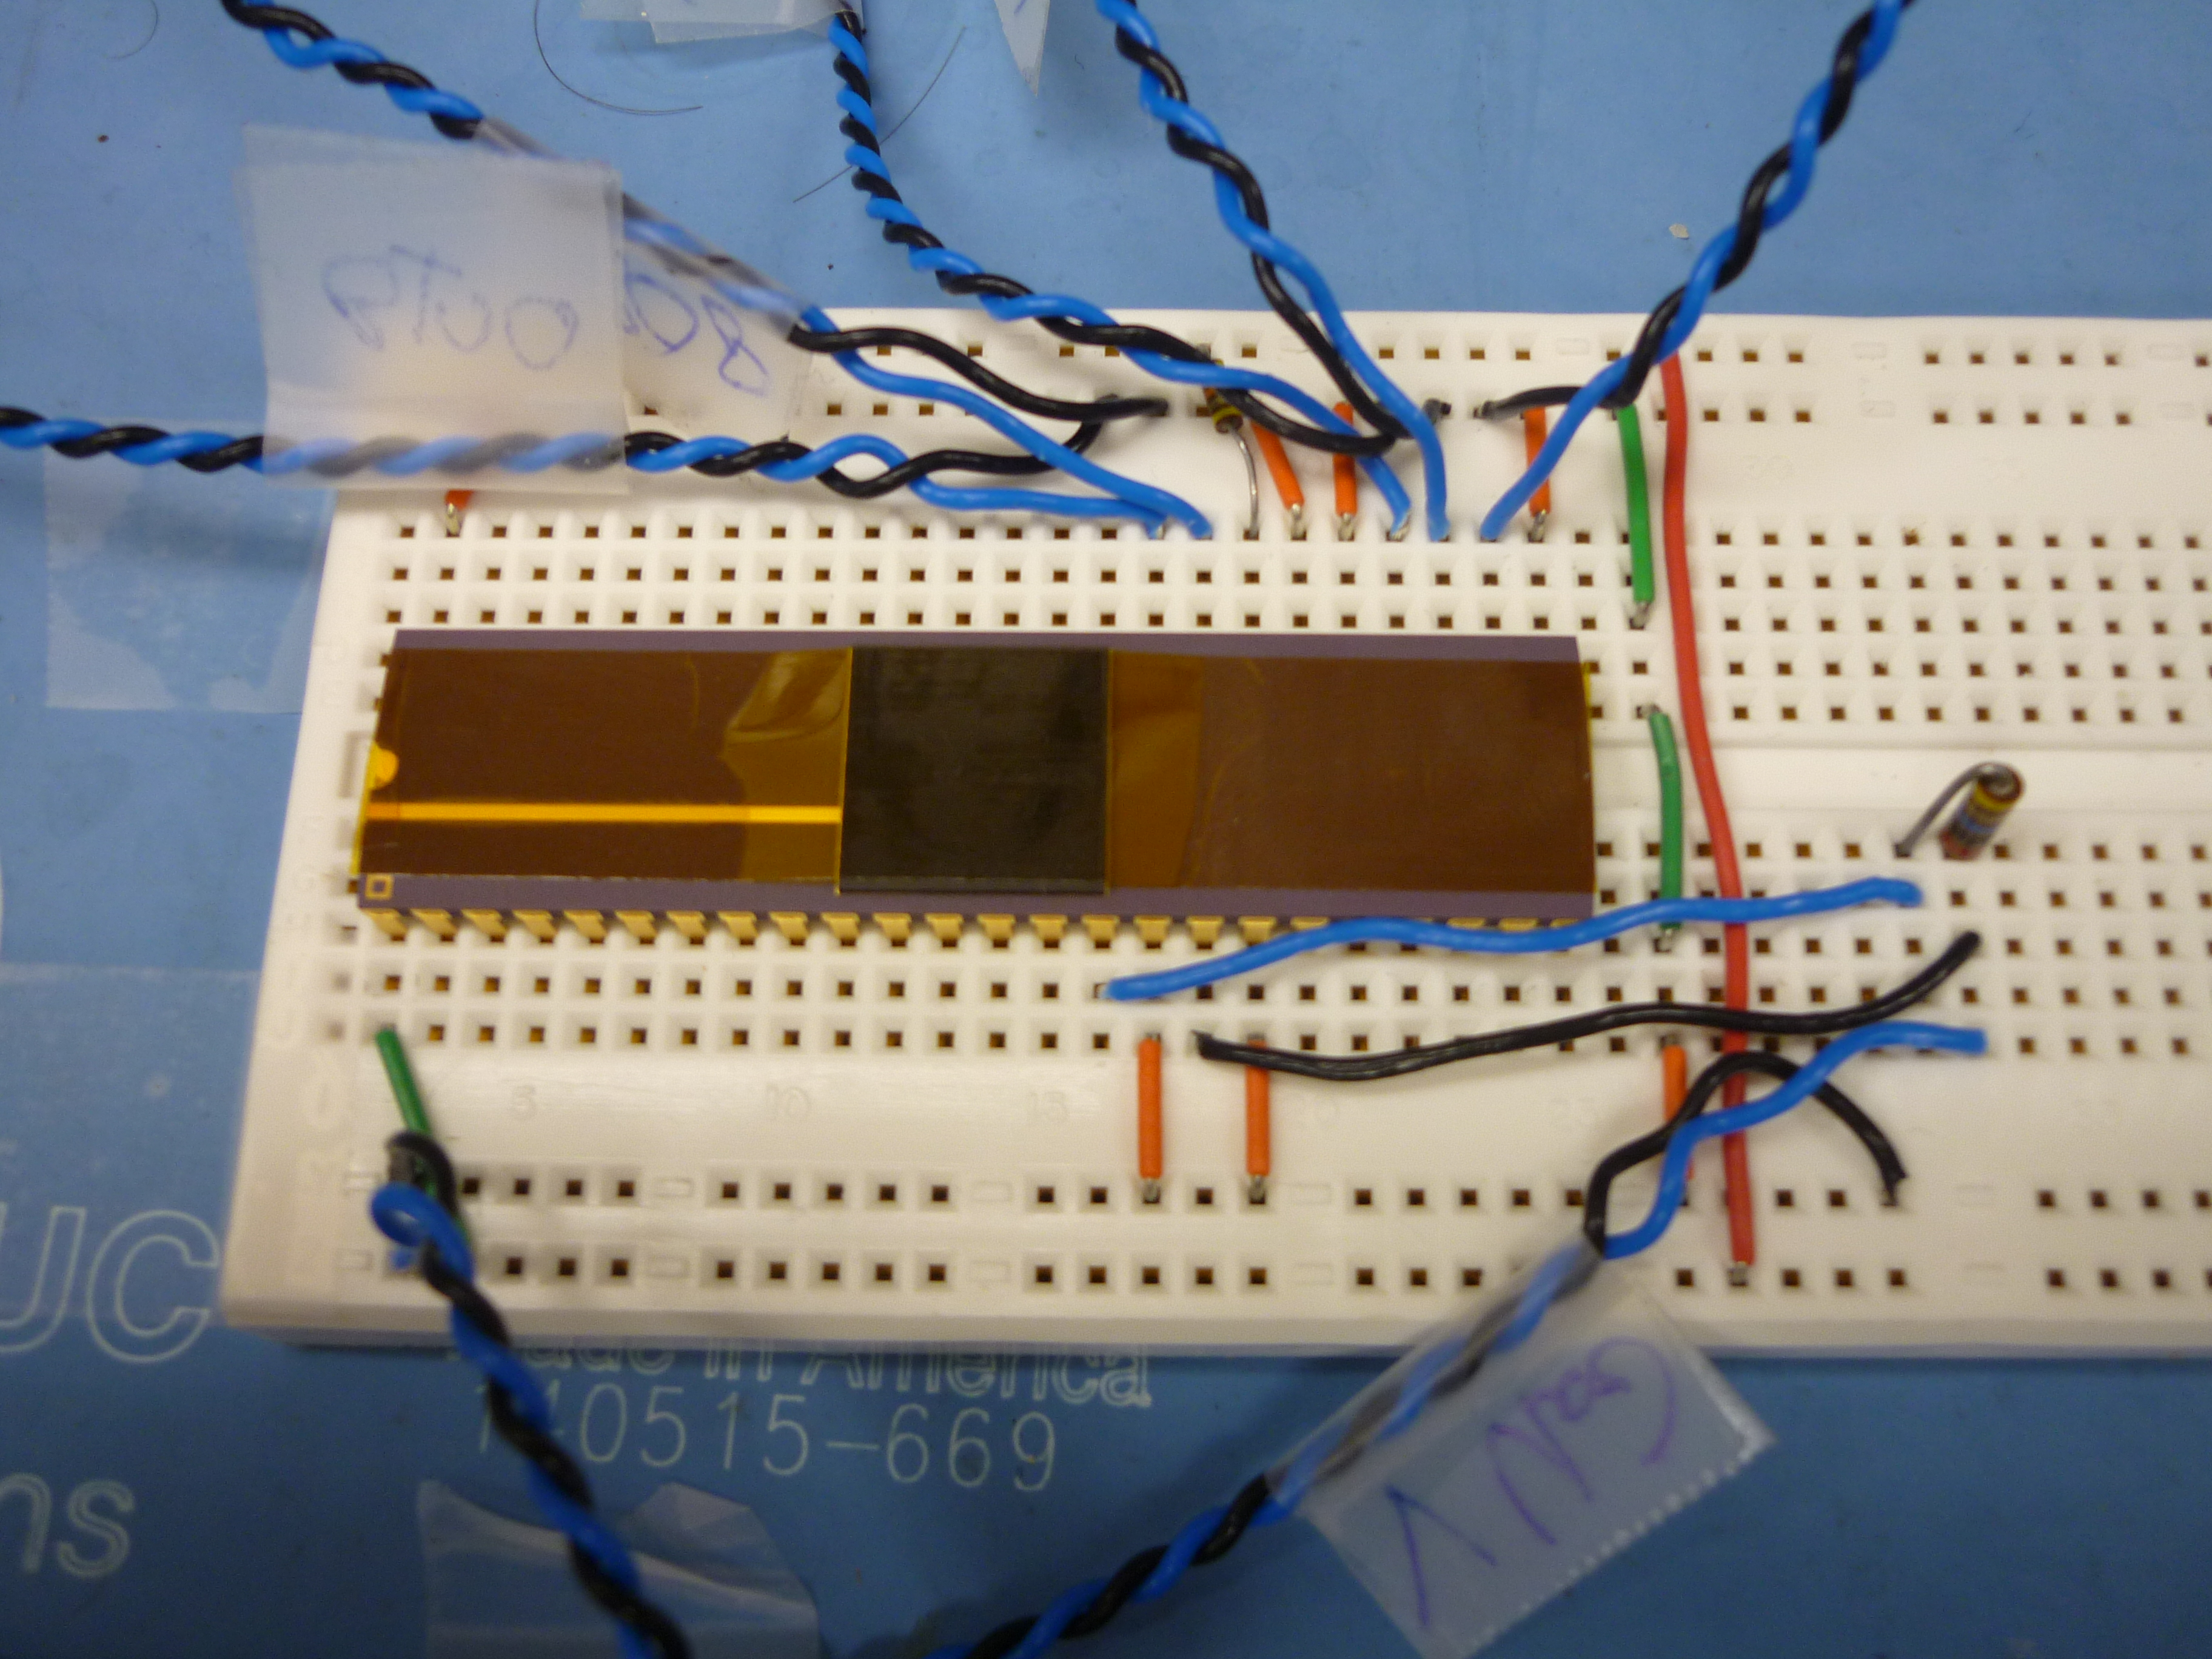
\includegraphics[width=0.6\linewidth]{fig/P1010159.JPG}
	\caption{close-up}
	\label{fig:close-up}
\end{figure}



\section{Characterization for high impedance voltage source}
This section aims to characterize the behavior of the ROIC while exposed to a voltage source with a high resistance in the order of several $M\Omega$. A focus is put onto the performance in reset state, the relationshiop between input current and output voltage, and the current limiting properties of the input transistor.

\subsection{Reset}
This mesaurement addresses the behavior of the circuit in reset mode. \Cref{tkz:schematic_ROIC_reset} shows the measured values during reset mode. Note that the input voltage is $2.4\,V$, which is important when calculating the input current. 

\begin{figure}[H]
\centering

\usetikzlibrary{shapes,snakes}

\newcommand*{\Vg}{Vg\\ $\color{red}4.5\,V$}
\newcommand*{\Rst}{Rst[3]\\ $\color{red}0\,V$} 
\newcommand*{\Res}{Res\\ $\color{red}0.86\,V$}
\newcommand*{\VDD}{VDD3.3\\ $\color{red}3.3\,V$}
\newcommand*{\IN}{IN[i]\\ $\color{red}2.4\,V$}
\newcommand*{\OUT}{OUT[i] $\color{red}1.4\,V$}
\newcommand*{\VBO}{VBO[i] $\color{red}1.4\,V$}
\newcommand*{\gnd}{gnd\\ $\color{red}0\,V$}
\newcommand*{\C}{$\color{red}450\,fF$}




\tikzstyle{dot} = [draw,shape=circle,fill=black, scale =.3]
\tikzstyle{l_arrow} = [draw,fill = black, regular polygon,regular polygon sides=3, rotate=-90, anchor=south, scale=.5] 
\tikzstyle{l_text} = [anchor=south west]
\tikzstyle{r_arrow} = [draw,fill = black, regular polygon,regular polygon sides=3, rotate=90, anchor=south, scale=.5] 
\tikzstyle{r_text} = [anchor=south east]
\begin{tikzpicture}[scale=1, every node/.style={scale=1}]




\draw[dashed]  (-0.5,5.5) rectangle (0.5,-2);
\node[align=center, anchor=south] at (0,5.5) {voltage\\limiter};

\draw[dashed]  (1.25,5.5) rectangle (5.25,-2);
\node[align=center, anchor=south] at (3.25,5.5) {integrator};

\draw[dashed]  (5.75,5.5) rectangle (9.25,-2);
\node[align=center, anchor=south] at (7.5,5.5) {current mirrors};

%\draw (0,0) to node[nfet]{};

%\draw (0,0) to (mos1.s);
\node(Vg)[nfet, rotate=-90] at (0,2.5) {};
\node[nfet, rotate=-90] (Reset) at (2.5,2) {};
\node[pfet] (CM_H1) at (5,3) {};
\node[nfet] (CM_L1) at (5,-1) {};
\node[nfet] (CM_H2) at (7,3) {};
\node[nfet] (CM_L2) at (7,-1) {};
\node[nfet] (CM_H3) at (9,3) {};
\node[nfet] (CM_L3) at (9,-1) {};



\draw (-1,2.5) node[anchor=east, align=center]{\IN} to (Vg.S);
\draw (Vg.G) |- (0,4.5) node[anchor=south, align=center]{\Vg};
\draw (Vg.B) |- (1,2.5) node[dot]{} |- (CM_H1.G); %top
\draw (1,2.5) |- (1,0.5)  to [C=\C](4,0.5) -| (CM_H1.D);
\draw (1.5,0.5) node[dot]{} -| (1.5,2) |- (Reset.B);
\draw (Reset.G) to (2.5,4.5) node[anchor=south, align=center]{\Rst};
\draw (Reset.D) -| (3.5,0.5) node[dot]{};
\draw (5,0.5) node[dot]{} to (CM_L1.D);
\draw (CM_L1.G) to (4,4.5) node[anchor=south, align=center]{\Res}; 
\draw (CM_L1.S) to (CM_L2.S) to (7,-2.5) node[anchor=north, align=center]{\gnd};
\draw (CM_H1.B) |- (CM_H2.D) to (7,4.5) node[anchor=south, align=center]{\VDD};
\draw (CM_L2.G) |- (4,0) node[dot]{};
\draw (5,0.5) -| (CM_H2.G);
\draw (CM_L1.B) to (CM_L1.S);
\draw (CM_L2.B) to (CM_L2.S);
\draw (CM_H2.B) to (CM_L2.D);
\draw (CM_H3.B) to (CM_L3.D);
\draw (1,3)node[dot]{} |- (8,4) |- (CM_H3.G);
\draw (CM_H3.D) |- (CM_H2.D) node[dot]{};
\draw (CM_L3.S) |- (CM_L2.S) node[dot]{};
\draw (CM_L3.G) |- (6,0) node[dot]{};
\draw (7,1.5)node[dot]{} to (10,1.5) node[anchor=west, align=center]{\OUT};
\draw (9,1)node[dot]{} to (10,1) node[anchor=west, align=center]{\VBO};




\end{tikzpicture}

\caption{Schematic of ROIC channel template}
\label{tkz:schematic_ROIC_reset}
\end{figure}



\subsection{Source follower}
There are two identical source followers per lane. We can use the VBO source follower to characterise both. This because the input can be directly controlled, and the output directly read. \Cref{fig:source_follower} shows both the measured data and a fitted line with the formula $vbo=0.827v_{in}-0.624$. It will be assumed that this line characterises the performance of both source followers for $1<v_{in}<4$.

\begin{figure}[h]
	    \centering
	    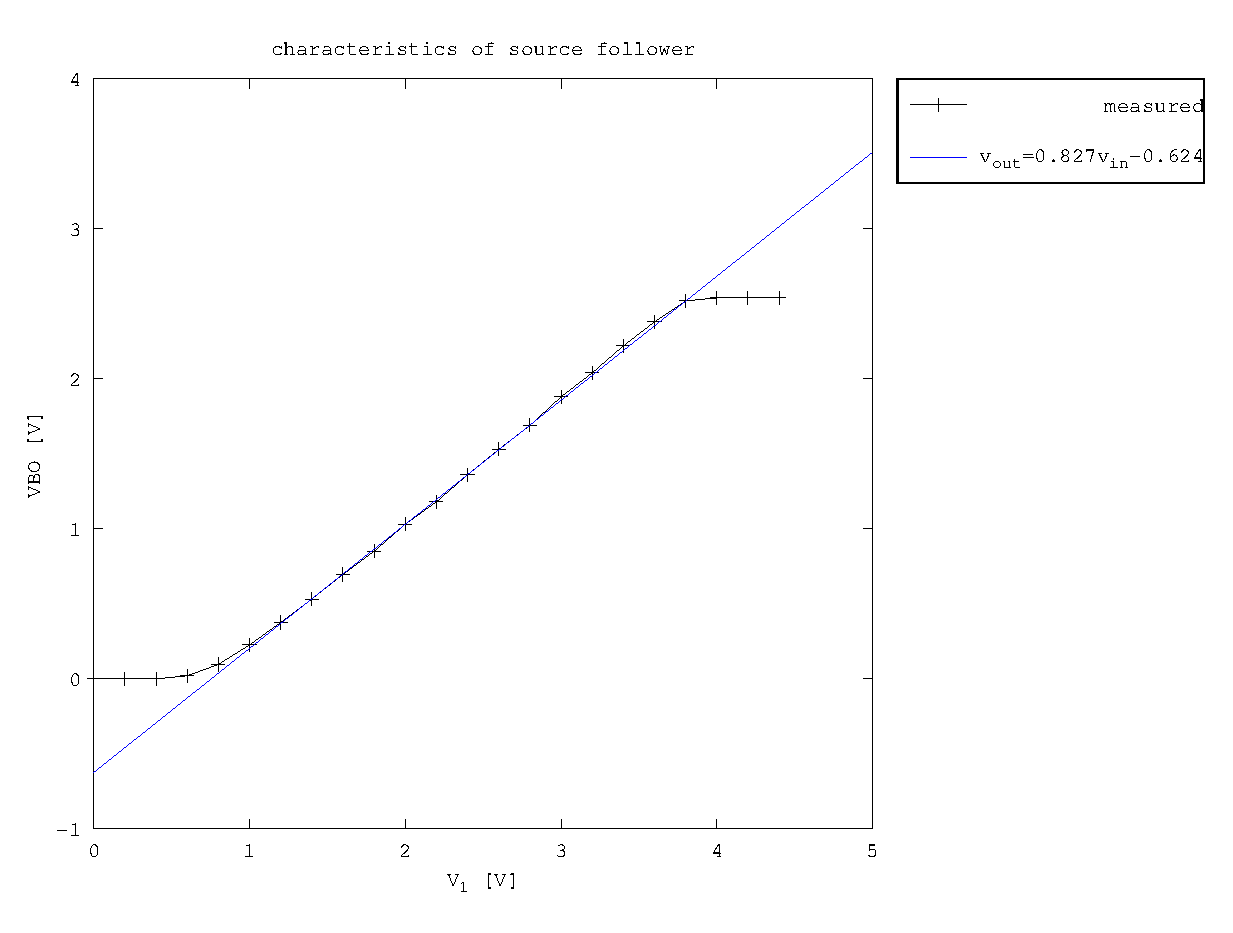
\includegraphics[width=\textwidth]{fig/source_follower.eps}
	    \caption[]%
	    {plot of the input voltage against VBO. This plot shows the characteristics of the voltage follower}    
	    \label{fig:source_follower}	
\end{figure}






\clearpage
\subsection{Standard performance}\label{ssec:standard}
This test aims to address the basic relationship between input current and output voltage. \Cref{tkz:integrator_test} shows the setup used for this test. Channel 8 was used, so the end of the $20\,M\Omega$ resistor is connected to IN[8], and probes are connected to OUT[8] and VBO[8]. 

\begin{figure}[H]
\centering

\usetikzlibrary{shapes,snakes}

\newcommand*{\Vg}{Vg\\ $\color{red}4.5\,V$}
\newcommand*{\Rst}{\textbf{Rst[3]}\\ $\color{blue}reset$} 
\newcommand*{\Res}{Res\\ $\color{red}0.86\,V$}
\newcommand*{\VDD}{VDD3.3\\ $\color{red}3.3\,V$}
\newcommand*{\IN}{$\color{blue}V_{in}$}
\newcommand*{\OUT}{$\color{blue}V_{out}$}
\newcommand*{\VBO}{\color{blue}\textbf{VBO[8]} $\color{red}1.4\,V$}
\newcommand*{\gnd}{gnd\\ $\color{red}0\,V$}
\newcommand*{\C}{$\color{blue}C$}




\tikzstyle{dot} = [draw,shape=circle,fill=black, scale =.3]
\tikzstyle{l_arrow} = [draw,fill = black, regular polygon,regular polygon sides=3, rotate=-90, anchor=south, scale=.5] 
\tikzstyle{l_text} = [anchor=south west]
\tikzstyle{r_arrow} = [draw,fill = black, regular polygon,regular polygon sides=3, rotate=90, anchor=south, scale=.5] 
\tikzstyle{r_text} = [anchor=south east]
\begin{tikzpicture}[scale=1, every node/.style={scale=1}]




\draw[dashed]  (-0.5,5.5) rectangle (0.5,-2);
\node[align=center, anchor=south] at (0,5.5) {voltage\\limiter};

\draw[dashed]  (1.25,5.5) rectangle (5.25,-2);
\node[align=center, anchor=south] at (3.25,5.5) {integrator};

\draw[dashed]  (5.75,5.5) rectangle (9.25,-2);
\node[align=center, anchor=south] at (7.5,5.5) {current mirrors};

%\draw (0,0) to node[nfet]{};

%\draw (0,0) to (mos1.s);
\node(Vg)[nfet, rotate=-90] at (0,2.5) {};
\node[nfet, rotate=-90] (Reset) at (2.5,2) {};
\node[pfet] (CM_H1) at (5,3) {};
\node[nfet] (CM_L1) at (5,-1) {};
\node[nfet] (CM_H2) at (7,3) {};
\node[nfet] (CM_L2) at (7,-1) {};
\node[nfet] (CM_H3) at (9,3) {};
\node[nfet] (CM_L3) at (9,-1) {};



\draw (-1,2.5) node[anchor=east, align=center]{} to (Vg.S);
\draw (Vg.G) |- (0,4.5) node[anchor=south, align=center]{\Vg};
\draw (Vg.B) |- (1,2.5) node[dot]{} |- (CM_H1.G); %top
\draw (1,2.5) |- (1,0.5)  to [C=\C](4,0.5) -| (CM_H1.D);
\draw (1.5,0.5) node[dot]{} -| (1.5,2) |- (Reset.B);
\draw (Reset.G) to (2.5,4.5) node[anchor=south, align=center]{\Rst};
\draw (Reset.D) -| (3.5,0.5) node[dot]{};
\draw (5,0.5) node[dot]{} to (CM_L1.D);
\draw (CM_L1.G) to (4,4.5) node[anchor=south, align=center]{\Res}; 
\draw (CM_L1.S) to (CM_L2.S) to (7,-2.5) node[anchor=north, align=center]{\gnd};
\draw (CM_H1.B) |- (CM_H2.D) to (7,4.5) node[anchor=south, align=center]{\VDD};
\draw (CM_L2.G) |- (4,0) node[dot]{};
\draw (5,0.5) -| (CM_H2.G);
\draw (CM_L1.B) to (CM_L1.S);
\draw (CM_L2.B) to (CM_L2.S);
\draw (CM_H2.B) to (CM_L2.D);
\draw (CM_H3.B) to (CM_L3.D);
\draw (1,3)node[dot]{} |- (8,4) |- (CM_H3.G);
\draw (CM_H3.D) |- (CM_H2.D) node[dot]{};
\draw (CM_L3.S) |- (CM_L2.S) node[dot]{};
\draw (CM_L3.G) |- (6,0) node[dot]{};
\draw (7,1.5)node[dot]{} to (10,1.5) node[anchor=west, align=center]{\OUT};
%\draw (9,1)node[dot]{} to (10,1) node[anchor=west, align=center]{\VBO};

\draw (-2.5,2.5)node[anchor=east, align=center]{\IN} to [R=$20\,M\Omega$](-1,2.5);


\end{tikzpicture}

\caption{Schematic of ROIC channel template}
\label{tkz:integrator_test}
\end{figure}


\Cref{fig:slopes} shows the time versus voltage plot of both the VBO and OUT for a constant input voltage. The rising and falling slopes are the VBO and OUt respecively. The timescale of this plot does not allow for much inside in VBO, but it does show some interesting results for the behavior of OUT. When the reset switches, the input node immediately loses some charge. Note that the osciloscope matches the rising edge of the rset signal to time is $0\,s$, so this drop is at $0\,s$. It is interesting to observe that the slope is constant for all input voltages. The slopes is much slower than the time necessary for the reset transistor to switch, so the observed slope is not limited by the reset transistor, but by the source follower that tries to keep up. This observed slope is therefore the maximum rate at which the output node can be pulled down in the current set-up.  lso note that the slope gets steeper when the integrator capacitance decreases. This is to be expected. However also note that the maximum slopes across the different capacitances are all identical.


\begin{figure}[h]
	\centering
	\begin{subfigure}[b]{0.475\textwidth}
	    \centering
	    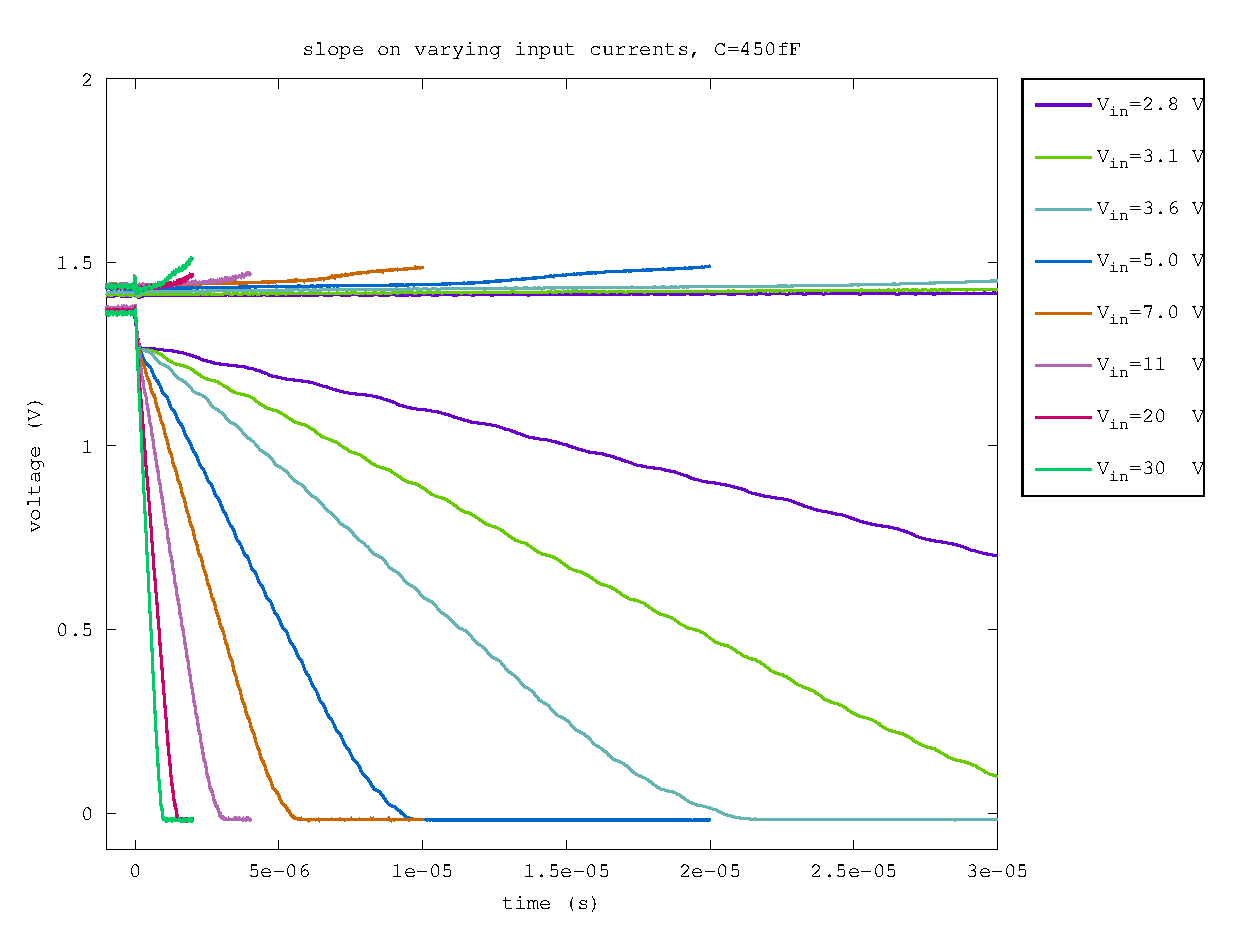
\includegraphics[width=\textwidth]{fig/slope_450fF.eps}
	    \caption[Network2]%
	    {$C=450\,fF$}    
	    \label{fig:slopes_450fF}
	\end{subfigure}
	\hfill
	\begin{subfigure}[b]{0.475\textwidth}  
	    \centering 
	    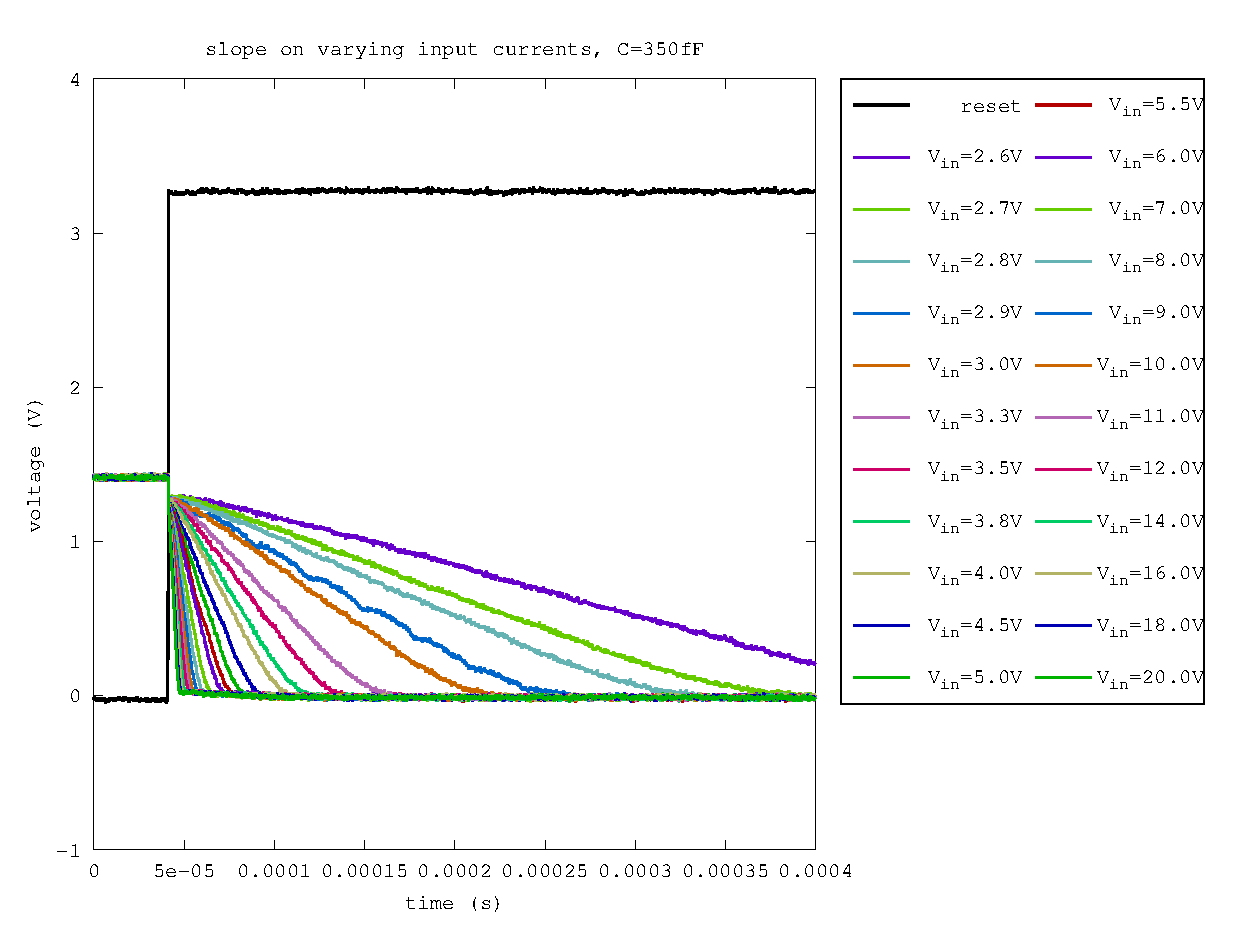
\includegraphics[width=\textwidth]{fig/slope_350fF.eps}
	    \caption[]%
	    {$C=350\,fF$}    
	    \label{fig:slopes_350fF}
	\end{subfigure}
	\vskip\baselineskip
	\begin{subfigure}[b]{0.475\textwidth}   
	    \centering 
	    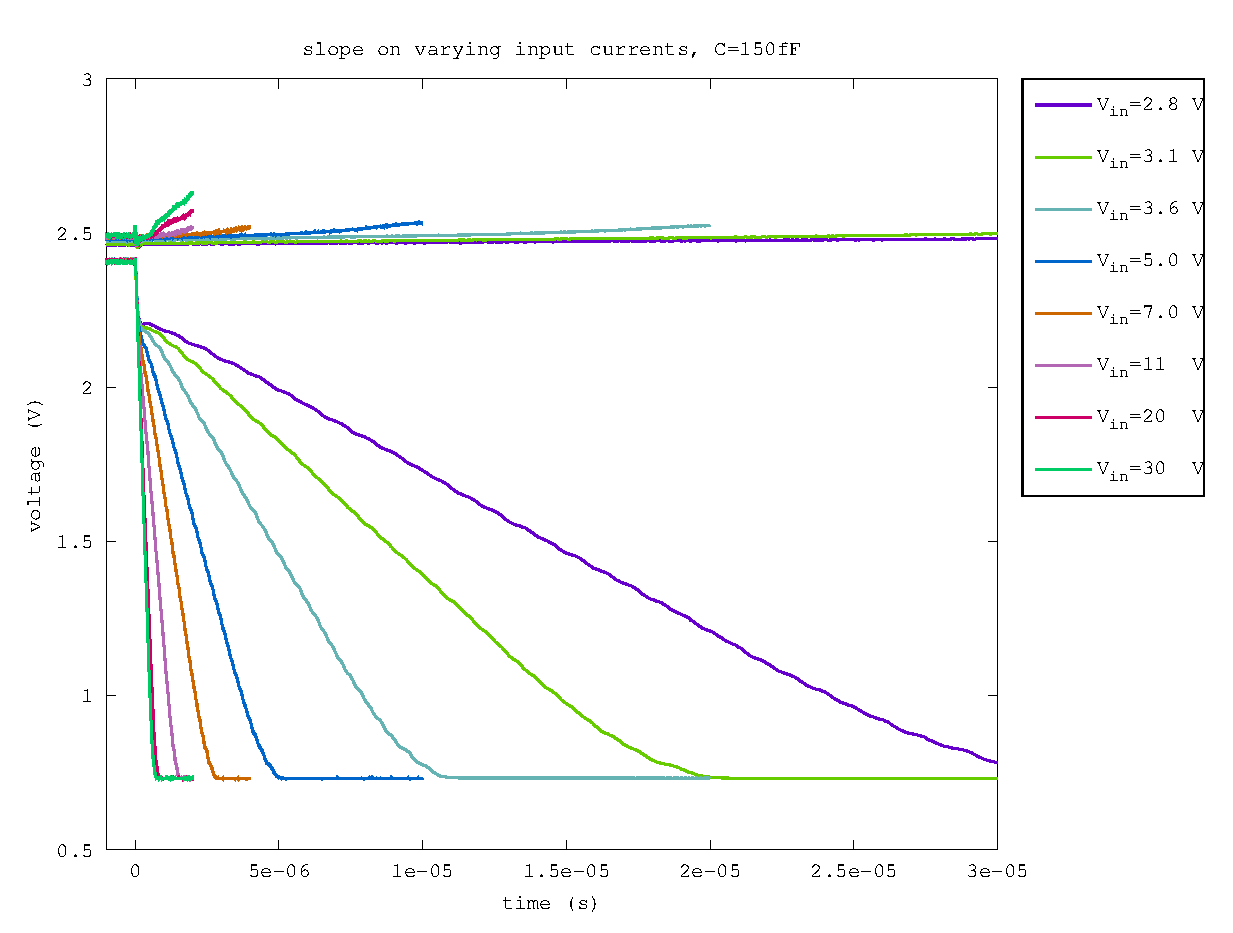
\includegraphics[width=\textwidth]{fig/slope_150fF.eps}
	    \caption[]%
	    {$C=150\,fF$}    
	    \label{fig:slopes_150fF}
	\end{subfigure}
	\quad
	\begin{subfigure}[b]{0.475\textwidth}   
	    \centering 
	    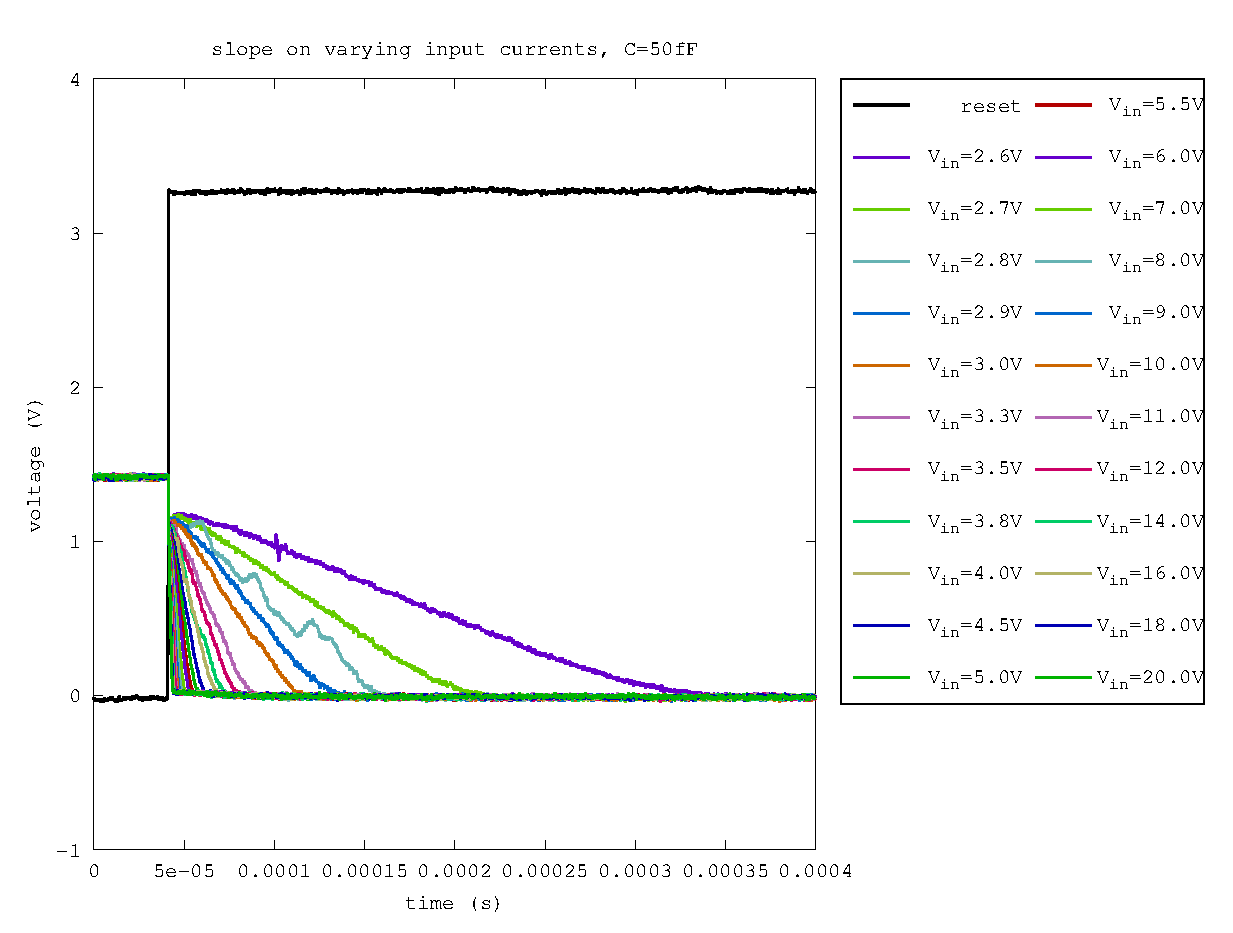
\includegraphics[width=\textwidth]{fig/slope_50fF.eps}
	    \caption[]%
	    {$C=50\,fF$}    
	    \label{fig:slopes_50fF}
	\end{subfigure}
	\caption{Expected versus measured charge up times for different input voltages. The input voltage is connected to the input through a resistor of $20\,M\Omega$}
	\label{fig:slopes}
\end{figure}

\Cref{fig:charges} shows the same plot as \cref{fig:slopes}, but now the x axis is scaled with input current. This shows for \cref{fig:slopes_450fF} and \ref{fig:slopes_350fF} that the relationship between output voltage and charge is equal across different input voltages. For \cref{fig:slopes_150fF} and \ref{fig:slopes_50fF} however, one can see that the higher voltages lose this property. Another intersting observation is that when one looks closely at the plot, one can observe a small oscillation with a period that is constant with charge. Also the period is constant across different voltages. A hypothesis explaining this behavior has yet to be found.


\begin{figure}[h]
	\centering
	\begin{subfigure}[b]{0.475\textwidth}
	    \centering
	    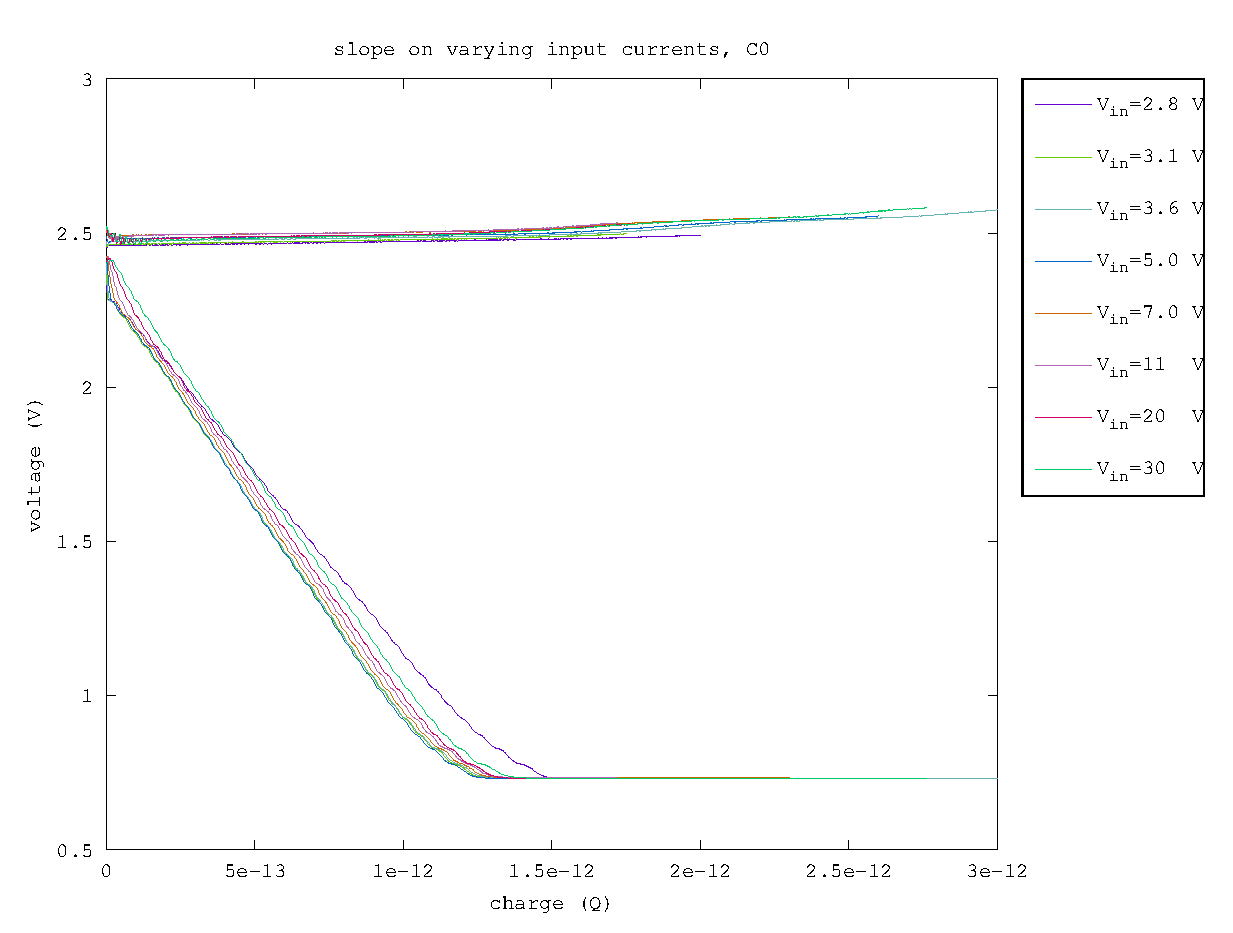
\includegraphics[width=\textwidth]{fig/charge_450fF.eps}
	    \caption[Network2]%
	    {$C=450\,fF$}    
	    \label{fig:charges_450fF}
	\end{subfigure}
	\hfill
	\begin{subfigure}[b]{0.475\textwidth}  
	    \centering 
	    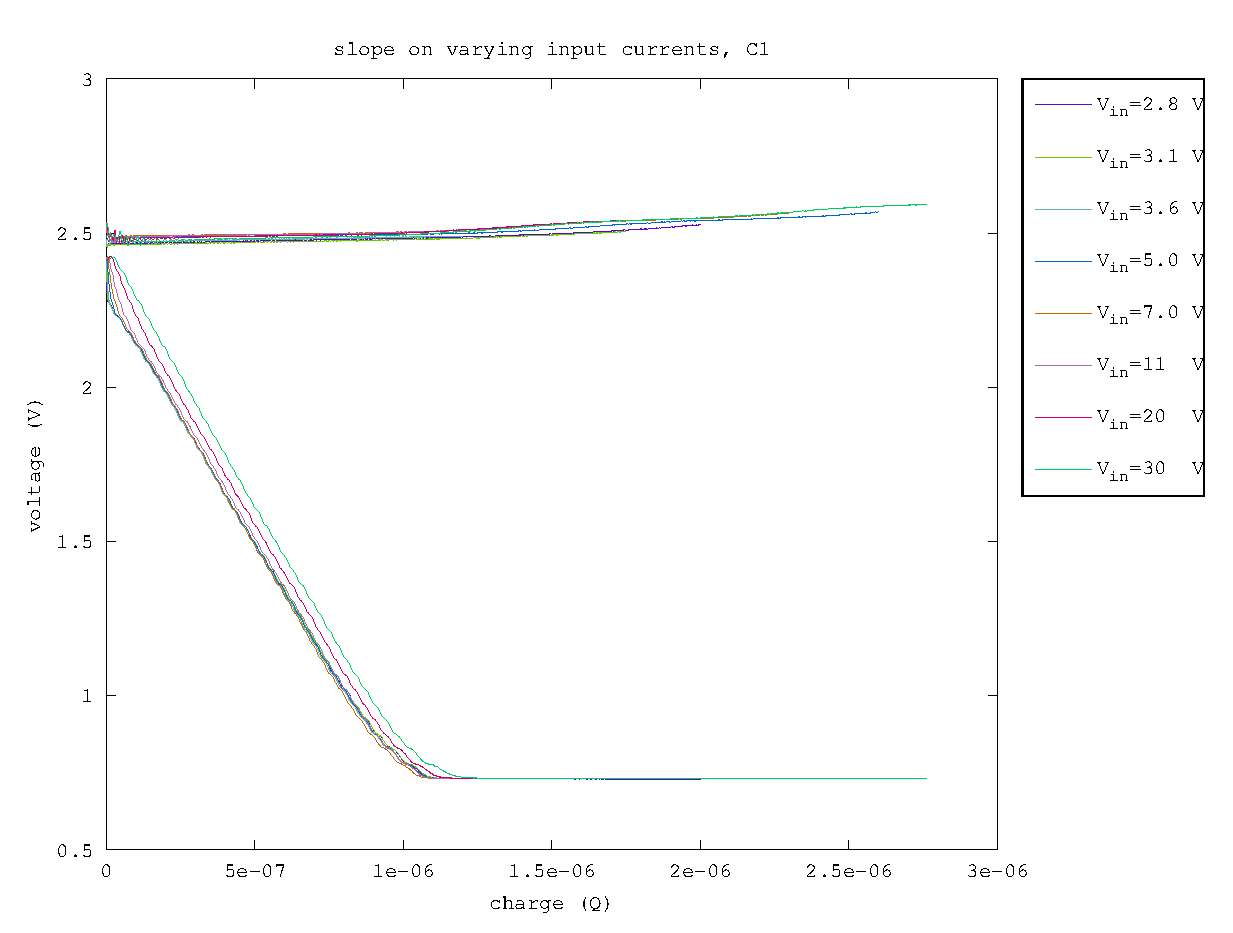
\includegraphics[width=\textwidth]{fig/charge_350fF.eps}
	    \caption[]%
	    {$C=350\,fF$}    
	    \label{fig:charges_350fF}
	\end{subfigure}
	\vskip\baselineskip
	\begin{subfigure}[b]{0.475\textwidth}   
	    \centering 
	    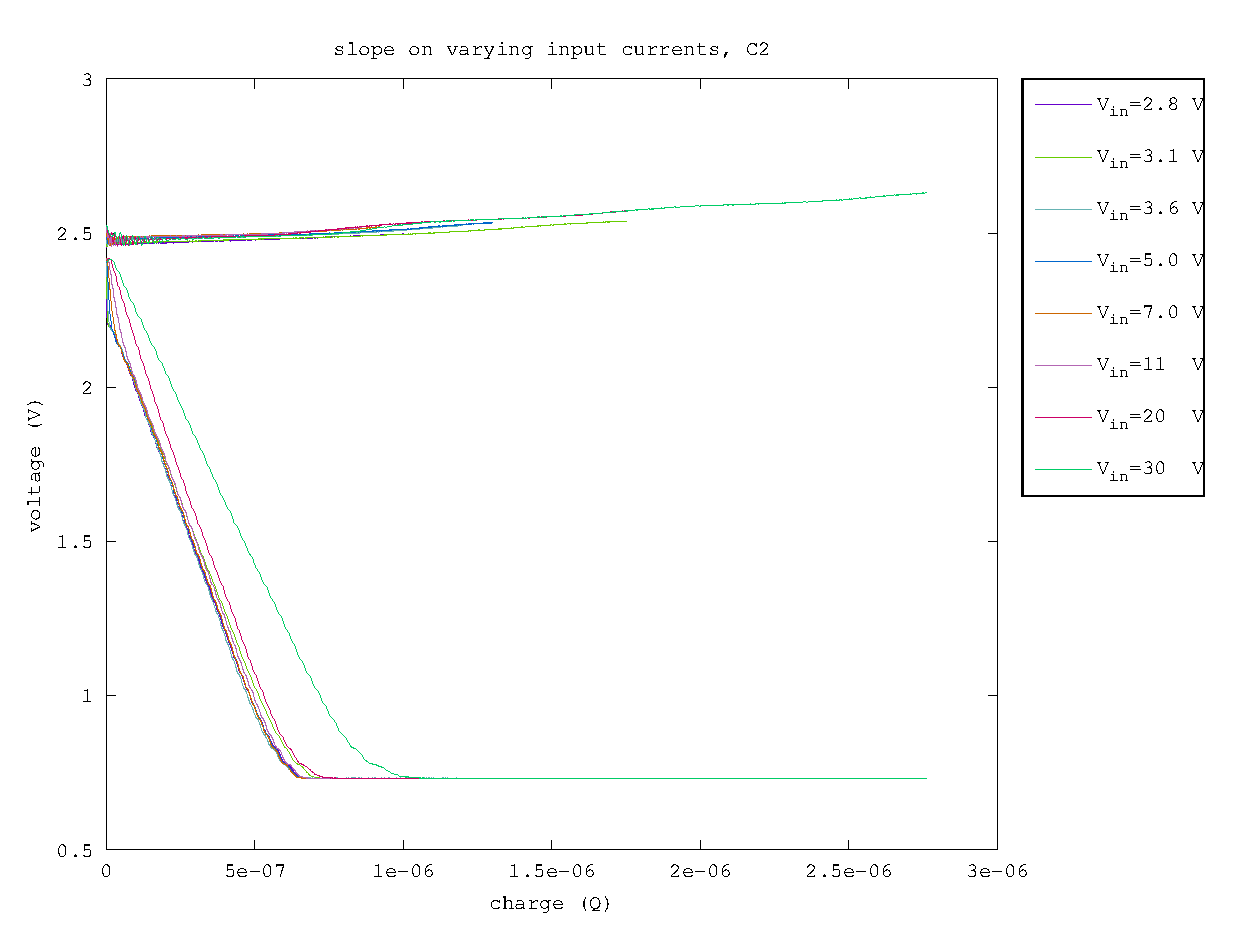
\includegraphics[width=\textwidth]{fig/charge_150fF.eps}
	    \caption[]%
	    {$C=150\,fF$}    
	    \label{fig:charges_150fF}
	\end{subfigure}
	\quad
	\begin{subfigure}[b]{0.475\textwidth}   
	    \centering 
	    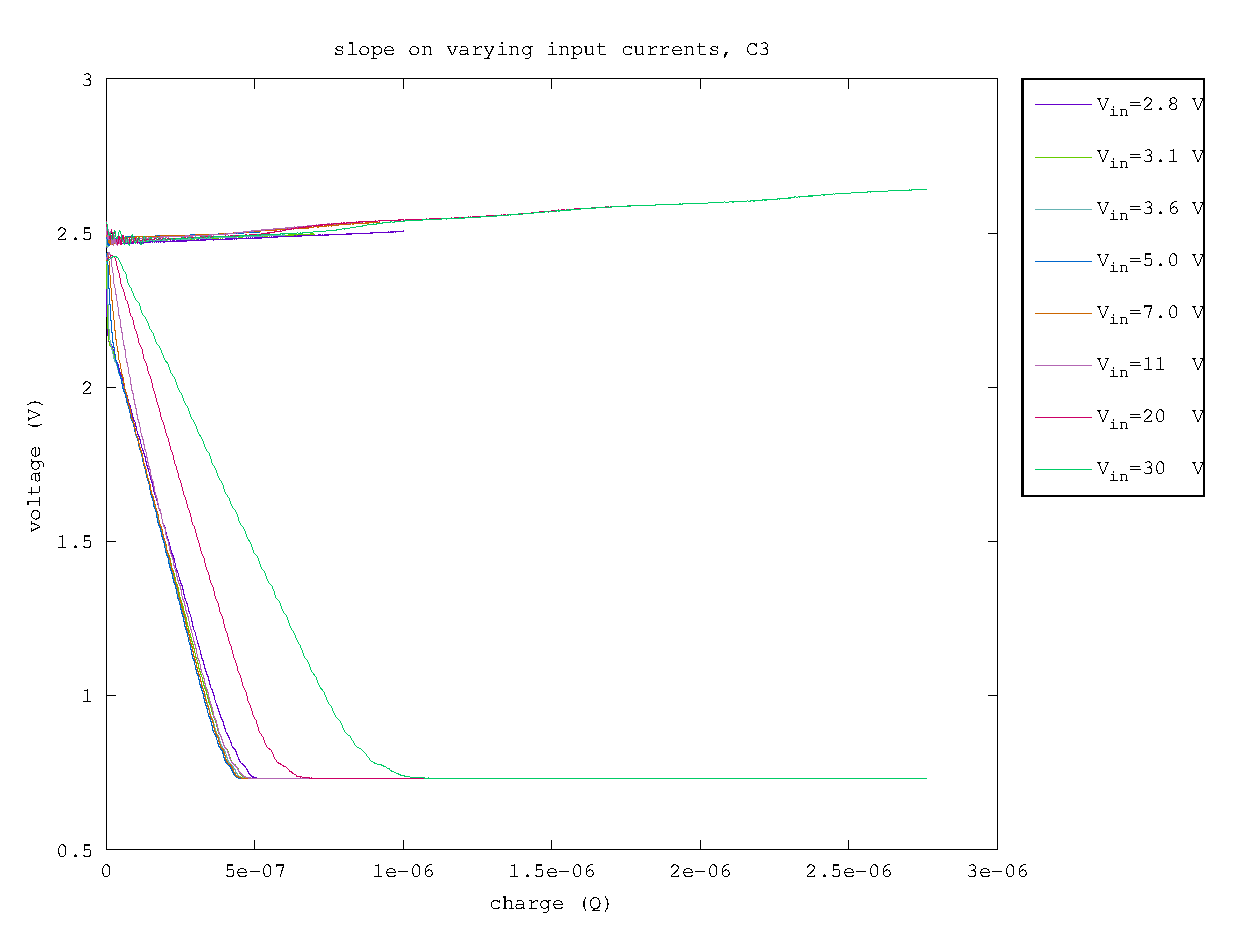
\includegraphics[width=\textwidth]{fig/charge_50fF.eps}
	    \caption[]%
	    {$C=50\,fF$}    
	    \label{fig:charges_50fF}
	\end{subfigure}
	\caption{This plot is showing charge versus voltage}
	\label{fig:charges}
\end{figure}

\Cref{fig:d_slopes} shows the $\delta Q/\delta V$ against charge plots. Note that $\delta Q/\delta V$ is the capacitance. One can observe that while the capacitance is charging, the full value of the capacitancec can be observed, and when the capacitance is comopletely decharged, it behaves as if it is not there. One can use these plots to estimate the integration capacitance. The capitance for \cref{fig:charges_450fF}, \ref{fig:charges_350fF}, \ref{fig:charges_150fF} and \ref{fig:charges_50fF} are approxiately $450\,fF$, $350\,fF$, $220\,fF$ and $180\,fF$ respectively.


\begin{figure}[h]
	\centering
	\begin{subfigure}[b]{0.475\textwidth}
	    \centering
	    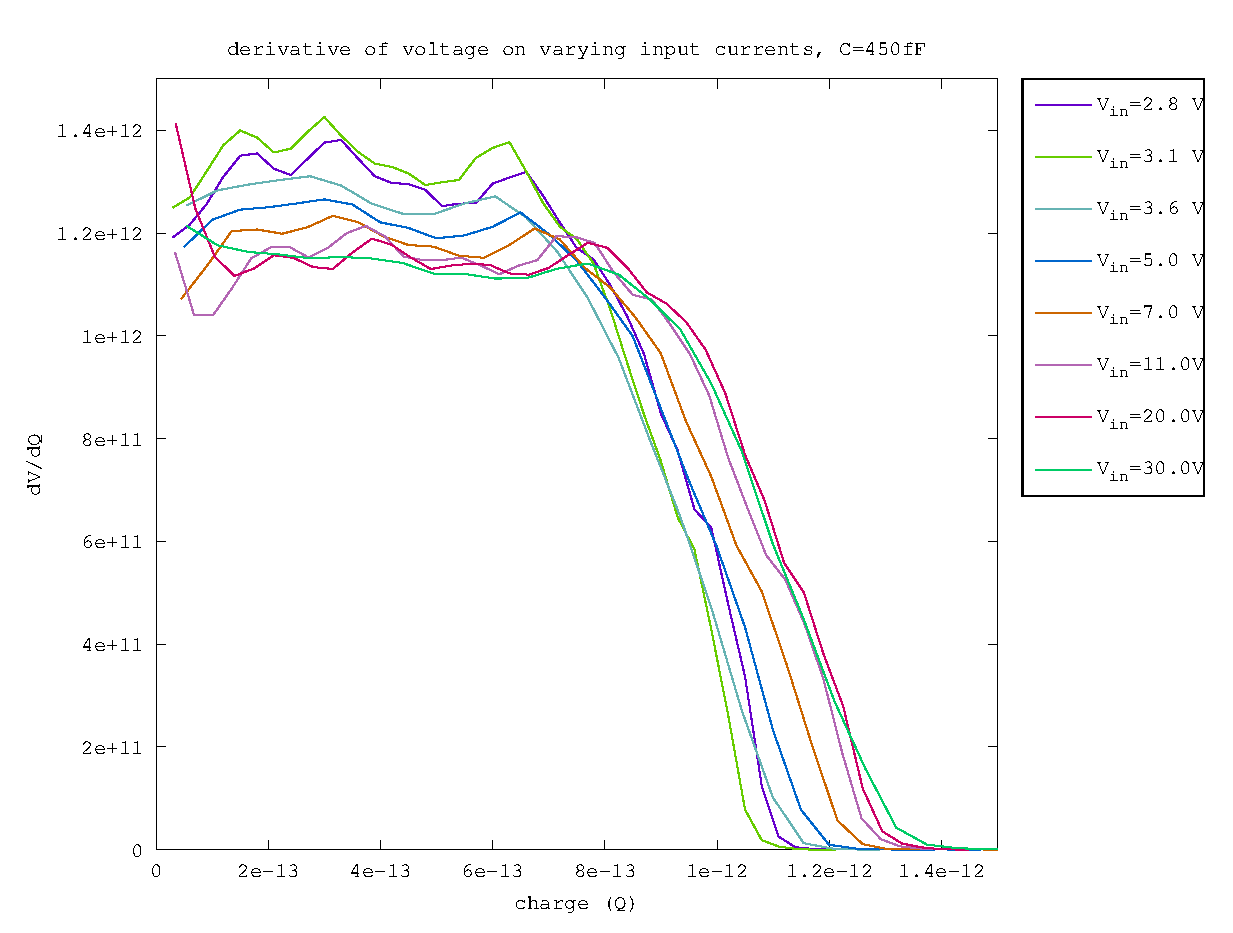
\includegraphics[width=\textwidth]{fig/d_slope_450fF.eps}
	    \caption[Network2]%
	    {$C=450\,fF$}    
	    \label{fig:d_slopes_450fF}
	\end{subfigure}
	\hfill
	\begin{subfigure}[b]{0.475\textwidth}  
	    \centering 
	    \includegraphics[width=\textwidth]{fig/d_slope_350fF.eps}
	    \caption[]%
	    {$C=350\,fF$}    
	    \label{fig:d_slopes_350fF}
	\end{subfigure}
	\vskip\baselineskip
	\begin{subfigure}[b]{0.475\textwidth}   
	    \centering 
	    \includegraphics[width=\textwidth]{fig/d_slope_150fF.eps}
	    \caption[]%
	    {$C=150\,fF$}    
	    \label{fig:d_slopes_150fF}
	\end{subfigure}
	\quad
	\begin{subfigure}[b]{0.475\textwidth}   
	    \centering 
	    \includegraphics[width=\textwidth]{fig/d_slope_50fF.eps}
	    \caption[]%
	    {$C=50\,fF$}    
	    \label{fig:d_slopes_50fF}
	\end{subfigure}
	\caption{The plot shows dv/dt against time. The plot is in log scale, which allows for an easy read on the maximum slope and the time needed to discharge the integrator capacitance. }
	\label{fig:d_slopes}
\end{figure}



\Cref{fig:e_vs_m} shows $\delta V / \delta t$ against input voltage for all capacitances. One can observe that all four have different slopes at first, but there appears to be a trend that they all converge to a value of $\delta V/\delta t \approx 3.2\cdot10^6$.


\begin{figure}[h]
	    \centering
	    \includegraphics[width=\textwidth]{fig/vin_vs_time_sat.eps}
	    \caption[]%
	    {dV/dt against input voltage for all four capacitances. The x indicate the measurements.}    
	    \label{fig:e_vs_m}	
\end{figure}



\clearpage
\subsection{large current performance}
In this section the $20\,M\Omega$ input resistor is replaecd with a $4\,M\Omega$ resistor. The main goal is to observe the ROIC for very large currents.


\Cref{fig:bre_slopes} shows the same plot as \cref{fig:slopes}, but this time with larger currents. Where a minimum slope could be observed at \cref{fig:slopes}, it is more prevalent here. This also shows more information about the behavior of VBO. For small voltages the VBO does not increase, but as the voltages get larger, one can observe that the voltages of VBO start rising when the OUT is done with decharging. It is also interesting to note that VBO seems to be not affected by the minimum slope at OUT. This gives rise to the hypothesis that the OUT is limited by the source follower. 

\begin{figure}[h]
	\centering
	\begin{subfigure}[b]{0.475\textwidth}
	    \centering
	    \includegraphics[width=\textwidth]{fig/bre_slope_450fF.eps}
	    \caption[Network2]%
	    {$C=450\,fF$}    
	    \label{fig:bre_slopes_450fF}
	\end{subfigure}
	\hfill
	\begin{subfigure}[b]{0.475\textwidth}  
	    \centering 
	    \includegraphics[width=\textwidth]{fig/bre_slope_350fF.eps}
	    \caption[]%
	    {$C=350\,fF$}    
	    \label{fig:bre_slopes_350fF}
	\end{subfigure}
	\vskip\baselineskip
	\begin{subfigure}[b]{0.475\textwidth}   
	    \centering 
	    \includegraphics[width=\textwidth]{fig/bre_slope_150fF.eps}
	    \caption[]%
	    {$C=150\,fF$}    
	    \label{fig:bre_slopes_150fF}
	\end{subfigure}
	\quad
	\begin{subfigure}[b]{0.475\textwidth}   
	    \centering 
	    \includegraphics[width=\textwidth]{fig/bre_slope_50fF.eps}
	    \caption[]%
	    {$C=50\,fF$}    
	    \label{fig:bre_slopes_50fF}
	\end{subfigure}
	\caption{Expected versus measured charge up times for different input voltages. The input voltage is connected to the input through a resistor of $4\,M\Omega$}
	\label{fig:bre_slopes}
\end{figure}

\Cref{fig:bre_charges} shows a similar plot as in \cref{fig:charges} but with higher currents. In \cref{fig:charges} one could observe that all currents fitted to the same line, but deviated at higher currents. This effect is also observed here, but in a stronger form. Which is to be expected.

\begin{figure}[h]
	\centering
	\begin{subfigure}[b]{0.475\textwidth}
	    \centering
	    \includegraphics[width=\textwidth]{fig/bre_charge_450fF.eps}
	    \caption[Network2]%
	    {$C=450\,fF$}    
	    \label{fig:bre_charges_450fF}
	\end{subfigure}
	\hfill
	\begin{subfigure}[b]{0.475\textwidth}  
	    \centering 
	    \includegraphics[width=\textwidth]{fig/bre_charge_350fF.eps}
	    \caption[]%
	    {$C=350\,fF$}    
	    \label{fig:bre_charges_350fF}
	\end{subfigure}
	\vskip\baselineskip
	\begin{subfigure}[b]{0.475\textwidth}   
	    \centering 
	    \includegraphics[width=\textwidth]{fig/bre_charge_150fF.eps}
	    \caption[]%
	    {$C=150\,fF$}    
	    \label{fig:bre_charges_150fF}
	\end{subfigure}
	\quad
	\begin{subfigure}[b]{0.475\textwidth}   
	    \centering 
	    \includegraphics[width=\textwidth]{fig/bre_charge_50fF.eps}
	    \caption[]%
	    {$C=50\,fF$}    
	    \label{fig:bre_charges_50fF}
	\end{subfigure}
	\caption{This plot is showing charge versus voltage}
	\label{fig:bre_charges}
\end{figure}

\Cref{fig:bre_d_slopes} shows a plot of $\delta V/\delta Q$ against charge. Note that the behavior for the low voltages differ across the different capacitances, but that the high voltages are not affected by a change in capacitance. This observation agrees with the hypothesis that the output is not limited by the input current, but by the speed of the source follower at the output.

\begin{figure}[h]
	\centering
	\begin{subfigure}[b]{0.475\textwidth}
	    \centering
	    \includegraphics[width=\textwidth]{fig/bre_d_slope_450fF.eps}
	    \caption[Network2]%
	    {$C=450\,fF$}    
	    \label{fig:bre_d_slopes_450fF}
	\end{subfigure}
	\hfill
	\begin{subfigure}[b]{0.475\textwidth}  
	    \centering 
	    \includegraphics[width=\textwidth]{fig/bre_d_slope_350fF.eps}
	    \caption[]%
	    {$C=350\,fF$}    
	    \label{fig:bre_d_slopes_350fF}
	\end{subfigure}
	\vskip\baselineskip
	\begin{subfigure}[b]{0.475\textwidth}   
	    \centering 
	    \includegraphics[width=\textwidth]{fig/bre_d_slope_150fF.eps}
	    \caption[]%
	    {$C=150\,fF$}    
	    \label{fig:bre_d_slopes_150fF}
	\end{subfigure}
	\quad
	\begin{subfigure}[b]{0.475\textwidth}   
	    \centering 
	    \includegraphics[width=\textwidth]{fig/bre_d_slope_50fF.eps}
	    \caption[]%
	    {$C=50\,fF$}    
	    \label{fig:bre_d_slopes_50fF}
	\end{subfigure}
	\caption{The plot shows dv/dt against time. The plot is in log scale, which allows for an easy read on the maximum slope and the time needed to discharge the integrator capacitance. }
	\label{fig:bre_d_slopes}
\end{figure}

\Cref{fig:bre_e_vs_m} shows the same plot as \cref{fig:e_vs_m}, but with higher current. This plot clearly shows that all four capacitance configurations saturate at a $\delta V\delta t \approx 3.1\,V$. This cannot be a limit applied to the input, because the capacitances are different. Therefore the output is limiting this, conform previous observations.

\begin{figure}[h]
	    \centering
	    \includegraphics[width=\textwidth]{fig/bre_vin_vs_time_sat.eps}
	    \caption[]%
	    {dV/dt against input voltage for all four capacitances. The x indicate the measurements.}    
	    \label{fig:bre_e_vs_m}	
\end{figure}

\clearpage
\subsection{Voltage limiter}
This section focusses on the output of the source follower that is directly connected to the output of the high voltage transistor connected to the input of the ROIC. The setup is identical to \cref{ssec:standard}, but the time scale is different to oberve the slower behavior of VBO.

\Cref{fig:vbo_slopes} shows the time against voltage plot. This are a couple of important observations that can be made from these plots. First and foremost: the behavior ofthe VBO is almost not affected by the capacitance. The behavior is fairly similar. There is a difference however, in that the VBO starts rising as the OUT reaches zero. This means that the VBO for $450\,fF$ is slightly delayed when compared to $50\,fF$ for example. It is also intersting yo observe that VBO never increases above $2.6\,V$. This behavior is most likely due to the high voltage input transistor doing it's job as a current limiter. Finally one can observe that for very low currents, VBO does not reach $2.6\,V$. The reason for this is that the input reaches the voltage level of the power supply before the current limiter kicks in.


\begin{figure}[h]
	\centering
	\begin{subfigure}[b]{0.475\textwidth}
	    \centering
	    \includegraphics[width=\textwidth]{fig/vbo_slope_450fF.eps}
	    \caption[Network2]%
	    {$C=450\,fF$}    
	    \label{fig:vbo_slopes_450fF}
	\end{subfigure}
	\hfill
	\begin{subfigure}[b]{0.475\textwidth}  
	    \centering 
	    \includegraphics[width=\textwidth]{fig/vbo_slope_350fF.eps}
	    \caption[]%
	    {$C=350\,fF$}    
	    \label{fig:vbo_slopes_350fF}
	\end{subfigure}
	\vskip\baselineskip
	\begin{subfigure}[b]{0.475\textwidth}   
	    \centering 
	    \includegraphics[width=\textwidth]{fig/vbo_slope_150fF.eps}
	    \caption[]%
	    {$C=150\,fF$}    
	    \label{fig:vbo_slopes_150fF}
	\end{subfigure}
	\quad
	\begin{subfigure}[b]{0.475\textwidth}   
	    \centering 
	    \includegraphics[width=\textwidth]{fig/vbo_slope_50fF.eps}
	    \caption[]%
	    {$C=50\,fF$}    
	    \label{fig:vbo_slopes_50fF}
	\end{subfigure}
	\caption{Expected versus measured charge up times for different input voltages. The input voltage is connected to the input through a resistor of $20\,M\Omega$}
	\label{fig:vbo_slopes}
\end{figure}

\Cref{fig:vbo_charges} shows the plots of voltage against charge. One can observe that increasing the current causes the behavior to converge to a line with a linear slope that is constant with Q, and a saturation at $2.6\,V$. 

\begin{figure}[h]
	\centering
	\begin{subfigure}[b]{0.475\textwidth}
	    \centering
	    \includegraphics[width=\textwidth]{fig/vbo_charge_450fF.eps}
	    \caption[Network2]%
	    {$C=450\,fF$}    
	    \label{fig:vbo_charges_450fF}
	\end{subfigure}
	\hfill
	\begin{subfigure}[b]{0.475\textwidth}  
	    \centering 
	    \includegraphics[width=\textwidth]{fig/vbo_charge_350fF.eps}
	    \caption[]%
	    {$C=350\,fF$}    
	    \label{fig:vbo_charges_350fF}
	\end{subfigure}
	\vskip\baselineskip
	\begin{subfigure}[b]{0.475\textwidth}   
	    \centering 
	    \includegraphics[width=\textwidth]{fig/vbo_charge_150fF.eps}
	    \caption[]%
	    {$C=150\,fF$}    
	    \label{fig:vbo_charges_150fF}
	\end{subfigure}
	\quad
	\begin{subfigure}[b]{0.475\textwidth}   
	    \centering 
	    \includegraphics[width=\textwidth]{fig/vbo_charge_50fF.eps}
	    \caption[]%
	    {$C=50\,fF$}    
	    \label{fig:vbo_charges_50fF}
	\end{subfigure}
	\caption{This plot is showing charge versus voltage}
	\label{fig:vbo_charges}
\end{figure}

\Cref{fig:vbo_d_slopes} shows $\delta V/\delta Q$ for the VBO. The main observation one can make fromthese plots is that the behavior of VBO is almost entirely unaffected by the integration capacitance.


\begin{figure}[h]
	\centering
	\begin{subfigure}[b]{0.475\textwidth}
	    \centering
	    \includegraphics[width=\textwidth]{fig/vbo_d_slope_450fF.eps}
	    \caption[Network2]%
	    {$C=450\,fF$}    
	    \label{fig:vbo_d_slopes_450fF}
	\end{subfigure}
	\hfill
	\begin{subfigure}[b]{0.475\textwidth}  
	    \centering 
	    \includegraphics[width=\textwidth]{fig/vbo_d_slope_350fF.eps}
	    \caption[]%
	    {$C=350\,fF$}    
	    \label{fig:vbo_d_slopes_350fF}
	\end{subfigure}
	\vskip\baselineskip
	\begin{subfigure}[b]{0.475\textwidth}   
	    \centering 
	    \includegraphics[width=\textwidth]{fig/vbo_d_slope_150fF.eps}
	    \caption[]%
	    {$C=150\,fF$}    
	    \label{fig:vbo_d_slopes_150fF}
	\end{subfigure}
	\quad
	\begin{subfigure}[b]{0.475\textwidth}   
	    \centering 
	    \includegraphics[width=\textwidth]{fig/vbo_d_slope_50fF.eps}
	    \caption[]%
	    {$C=50\,fF$}    
	    \label{fig:vbo_d_slopes_50fF}
	\end{subfigure}
	\caption{The plot shows dv/dt against time of the vbo.}
	\label{fig:vbo_d_slopes}
\end{figure}


\Cref{fig:vbo_e_vs_m} shows the $\delta V/\delta t$ against input voltage for VBO across all capacitances. For large voltages seem to behave in a noemal linear fashon. The startup shows a scene that looks as if the $450\,fF$ and $350\,fF$ setup behave identical, and that the $150\,fF$ and $50\,fF$ setup behave identical. This might be due to the lack of measurement points, but is worth investigating further.



\begin{figure}[h]
	    \centering
	    \includegraphics[width=\textwidth]{fig/vbo_vin_vs_time_sat.eps}
	    \caption[]%
	    {dV/dt of VBO against input voltage for all four capacitances. The x indicate the measurements.}    
	    \label{fig:vbo_e_vs_m}	
\end{figure}


\Cref{fig:vg_vs_vbo} shows the relationship between $V_g$ and the voltage limit posed by the high voltage transistor at the input. 

\begin{figure}[h]
	    \centering
	    \includegraphics[width=\textwidth]{fig/vg_vs_vbo.eps}
	    \caption[]%
	    {voltage limit as a function of Vg}    
	    \label{fig:vg_vs_vbo}	
\end{figure}





\clearpage





\section{Characterization of GaN sensors}
After the ROIc is characterized, it can be put to use by measuring the GaN sensors it is designed for. However, before starting on the GaN sensors, the device first gets an upgrade. This time, labVIEW is used to control and readout the oscilloscope in real time. This time the reset signal is not generated by the oscilloscope, but by a seperate function generator. This leaves room for the function generator on the oscilloscope to drive the input voltage. Using the oscilloscope and a voltage amplifier, a range of 0 to $25\,V$ can be achieved. The main advantage is that this range can be controlled in labVIEW, which enables an automatic programmed voltage sweep. 

This measurement method is used to measure the performance of the different sensors in forward bias. The result of his is shown in \cref{fig:pin26-40}. The VBO channel is used for the measurements because of the large currents. There are several oberservations that be made using this plot. First of all, there are several pins that appear to be unaffected by the input voltage. This is not due to the GaN sensors, but because the ROIC channel broke after a certain point. This is most likely because the input was accidently connected to a ground pin, which puts the high voltage directly to the input of the ROIC. A second observation is that the reset value of the VBO cannotr be contained for large input voltages. This most likely means that the amount of current that is put into the ROIC is larger than the opamp in the ROIC can keep up with. Using an external current meter, the maximum amount of current the opamp can compete with is approximately $15\,\mu A$. Finally it is interesting to observe that there is a substantial variance across the different devices. In order to test whether this variance is due to noise or due to variance across devices, a second set of measurements are made, but this time on a single device. The results are shown in \cref{fig:pin32}. These measurements show that the variance over different measurements is relatively low, and that the observed variance in \cref{fig:pin26-40} is actually caused by variance across different devices.


\begin{figure}[h]
	\centering
	\begin{subfigure}[b]{0.475\textwidth}
	    \centering
	    \includegraphics[width=\textwidth]{fig/pin26-40_slope_0-25V.eps}
	    \caption[Network2]%
	    {I/V characteristics}    
	    \label{fig:pin26-40_slope}
	\end{subfigure}
	\hfill
	\begin{subfigure}[b]{0.475\textwidth}  
	    \centering 
	    \includegraphics[width=\textwidth]{fig/pin26-40_reset_0-25V.eps}
	    \caption[]%
	    {reset value for VBO}    
	    \label{fig:pin26-40_reset}
	\end{subfigure}
	\caption{The slope and reset values for the VBO of pin26-40}
	\label{fig:pin26-40}
\end{figure}

\begin{figure}[h]
	\centering
	\begin{subfigure}[b]{0.475\textwidth}
	    \centering
	    \includegraphics[width=\textwidth]{fig/pin32_slope_0-25V.eps}
	    \caption[Network2]%
	    {I/V characteristics}    
	    \label{fig:pin32_slope}
	\end{subfigure}
	\hfill
	\begin{subfigure}[b]{0.475\textwidth}  
	    \centering 
	    \includegraphics[width=\textwidth]{fig/pin32_reset_0-25V.eps}
	    \caption[]%
	    {reset value for VBO}    
	    \label{fig:pin32_reset}
	\end{subfigure}
	\caption{The slope and reset values for the VBO of pin32 repeated multiple times to test variance across measurements}
	\label{fig:pin32}
\end{figure}


The next step is to investigate reverse bias, and to achieve that the ground and pin input of the GaN sensor are switched around. The I/V characteristics for several pins are shown in \cref{fig:pin22_30_slope}. The jumps to negative current between 0 and $2.4\,V$ is due to the ROIC being $2.4\,V$. Therefore for lower voltages, the current flows into the opposite direction. The numbers are not representative for the actual current though, because the ROIC and measurement method are not designed for that direction of current. The main observation that can be made is that the voltage range available in the current setup is insufficient to observe the most intersting part of the I/V characteristics.  

\begin{figure}[h]
	    \centering
	    \includegraphics[width=\textwidth]{fig/pin22-30_slope_-25-0V.eps}
	    \caption[]%
	    {Voltage to current characteristics for several GaN sensors}    
	    \label{fig:pin22_30_slope}	
\end{figure}  


\subsection{High voltage range I/V characteristics}
In order to get a higher voltage range, tghe setup is changed again. The amplifier used for the input voltage caused a lot of noise and did not amplify enough. The new setup uses a manually controlled voltage source as input voltage. The input voltage is also measured by the oscilloscope. labVIEW continuesly takes measurements where it extracts both the current voltage and current. By manually sweeping the input voltage one can accumulate data points to construct the I/V characteristics. The I/V characteristics for pin 21 on the chip are shown in



\begin{figure}[h]
	    \centering
	    \includegraphics[width=\textwidth]{fig/pin21_slope.eps}
	    \caption[]%
	    {Voltage to current characteristics for several GaN sensors}    
	    \label{fig:pin22_30_slope}	
\end{figure}  





\end{document}



